\documentclass{article}
\usepackage[utf8]{inputenc}
\usepackage{enumitem, amsfonts, subcaption, indentfirst, rotating, tikz, lscape, amssymb, hyperref, longtable, float, amsmath, graphicx, multicol, multirow, booktabs}
\usepackage[margin=.5in]{geometry}
\usetikzlibrary{quotes}
\usetikzlibrary{positioning}

\title{Data Source Report}

\author{Scott Kjorlien}
\date{\today}

\begin{document}
\maketitle

\section*{Introduction} 
The previous GSR for this project filed a FOIA request for US Farm Payments data in early 2022. After this project received 
the discs with data files in excel format (FOIA Data), USDA published all of the data on 
\href{https://www.fsa.usda.gov/news-room/efoia/electronic-reading-room/frequently-requested-information/payment-files-information/index}{their website} 
(Public Data).\\

The purpose of this report is to analyze and document differences between the data sources, and determine the path forward: 
continue periodically requesting data through the FOIA process, or switch to the Publicly available data.

\section*{Summary Statistics}
The tables below show annualized summary statistics for the two sources of data. Upon first glance, we see that the public 
data extends the horizon back to 2004 and up to 2022. It remains to be seen how complete those years' data are. However, 
judging by the count of records, 2021 appears to be rather incomplete in the FOIA data with 80K records as opposed to the 4M records 
in the public data. \\

From 2006 through 2009, all summary statistics are identical. From then on, however, we have more records, higher totals, 
weakly higher maxima, and generally higher sums in the Public Data. \\ 
This implies the public data is more complete, but it is unclear what was missing from the FOIA data. 


\subsection*{FOIA Data Summary}
\begin{table}[H]
\caption{Summary Stats from FOIA data}
\begin{tabular}{lrrrrr}
\toprule
 & \multicolumn{5}{r}{payment} \\
 & mean & max & sum & std & count \\
year &  &  &  &  &  \\
\midrule
2006 & \$ 788.06 & \$ 91,720.16 & \$ 441,395,789.32 & \$ 1,676.05 & 560102 \\
2007 & \$ 352.16 & \$ 25,273.56 & \$ 74,762,121.50 & \$ 864.11 & 212296 \\
2008 & \$ 867.34 & \$ 668,810.00 & \$ 10,207,878,350.00 & \$ 2,967.92 & 11769158 \\
2009 & \$ 2,022.60 & \$ 697,812.00 & \$ 9,992,060,725.00 & \$ 4,625.21 & 4940213 \\
2010 & \$ 1,606.34 & \$ 1,086,026.00 & \$ 10,615,437,806.00 & \$ 5,096.92 & 6608477 \\
2011 & \$ 1,470.96 & \$ 1,911,038.00 & \$ 7,853,899,680.98 & \$ 4,967.86 & 5339306 \\
2012 & \$ 2,178.24 & \$ 2,266,952.00 & \$ 8,055,749,016.28 & \$ 6,030.28 & 3698290 \\
2013 & \$ 2,271.05 & \$ 2,170,375.00 & \$ 7,470,720,100.00 & \$ 7,338.33 & 3289544 \\
2014 & \$ 4,208.69 & \$ 5,575,000.00 & \$ 7,179,329,103.00 & \$ 12,448.26 & 1705836 \\
2015 & \$ 3,363.29 & \$ 4,770,000.00 & \$ 8,333,282,360.00 & \$ 8,294.39 & 2477720 \\
2016 & \$ 3,071.41 & \$ 2,255,666.00 & \$ 10,711,725,040.00 & \$ 7,262.81 & 3487563 \\
2017 & \$ 2,968.00 & \$ 2,072,055.00 & \$ 9,527,872,811.00 & \$ 7,634.21 & 3210198 \\
2018 & \$ 3,400.24 & \$ 952,719.00 & \$ 11,600,600,872.59 & \$ 9,075.45 & 3411698 \\
2019 & \$ 4,878.41 & \$ 1,500,000.00 & \$ 19,979,521,019.04 & \$ 14,411.92 & 4095496 \\
2020 & \$ 4,892.06 & \$ 3,141,886.78 & \$ 37,812,702,107.61 & \$ 18,662.83 & 7729400 \\
2021 & \$ 9,509.09 & \$ 1,495,778.52 & \$ 762,857,586.43 & \$ 30,556.64 & 80224 \\
\bottomrule
\end{tabular}
\end{table}


\subsection*{Public Data Summary}
\begin{table}[H]
\caption{Summary Stats from Public data}
\begin{tabular}{lrrrrr}
\toprule
 & \multicolumn{5}{r}{payment} \\
 & mean & max & sum & std & count \\
year &  &  &  &  &  \\
\midrule
2004 & \$ 1,993.27 & \$ 19,020.68 & \$ 211,287.05 & \$ 3,312.42 & 106 \\
2005 & \$ 1,858.11 & \$ 347,834.20 & \$ 1,239,418,612.72 & \$ 4,715.05 & 667033 \\
2006 & \$ 788.06 & \$ 91,720.16 & \$ 441,395,789.32 & \$ 1,676.05 & 560102 \\
2007 & \$ 352.16 & \$ 25,273.56 & \$ 74,762,121.50 & \$ 864.11 & 212296 \\
2008 & \$ 867.34 & \$ 668,810.00 & \$ 10,207,879,211.09 & \$ 2,967.92 & 11769158 \\
2009 & \$ 2,022.60 & \$ 697,812.00 & \$ 9,992,061,451.50 & \$ 4,625.21 & 4940213 \\
2010 & \$ 1,654.83 & \$ 4,925,876.00 & \$ 10,965,568,866.50 & \$ 7,522.88 & 6626408 \\
2011 & \$ 1,560.55 & \$ 5,000,000.00 & \$ 8,855,627,288.19 & \$ 7,734.06 & 5674683 \\
2012 & \$ 2,223.25 & \$ 5,000,000.00 & \$ 8,770,993,864.65 & \$ 9,345.58 & 3945131 \\
2013 & \$ 2,305.05 & \$ 4,000,000.00 & \$ 9,017,546,913.82 & \$ 9,509.81 & 3912079 \\
2014 & \$ 4,340.19 & \$ 5,575,000.00 & \$ 7,806,551,895.88 & \$ 15,419.75 & 1798664 \\
2015 & \$ 3,393.23 & \$ 4,770,000.00 & \$ 8,989,304,069.96 & \$ 10,954.09 & 2649186 \\
2016 & \$ 3,101.87 & \$ 6,000,000.00 & \$ 11,508,682,520.04 & \$ 12,510.59 & 3710243 \\
2017 & \$ 3,012.22 & \$ 3,955,922.00 & \$ 10,263,637,351.99 & \$ 10,930.82 & 3407337 \\
2018 & \$ 3,537.25 & \$ 94,000,000.00 & \$ 12,751,250,456.50 & \$ 92,089.58 & 3604845 \\
2019 & \$ 4,848.17 & \$ 3,500,000.00 & \$ 20,896,707,040.36 & \$ 15,848.31 & 4310226 \\
2020 & \$ 4,980.09 & \$ 82,324,957.00 & \$ 39,357,702,923.99 & \$ 80,209.21 & 7903003 \\
2021 & \$ 4,069.86 & \$ 9,924,038.00 & \$ 16,422,246,507.68 & \$ 14,343.61 & 4035087 \\
2022 & \$ 7,240.45 & \$ 4,243,602.50 & \$ 13,187,642,193.08 & \$ 22,089.06 & 1821385 \\
\bottomrule
\end{tabular}
\end{table}


\section*{Difference Tables}
The following pages include two tables of a similar flavor. Since we find above that Public Data appears to be more complete than 
the FOIA data, here we analyze the difference between Public and FOIA for each state by year (see \autoref{stateYearDiffTable}) 
followed by program by year (see \autoref{progYearDiffTable}). These figures are shown in Millions of USD to 
examine which categories contribute most to the difference between the two data sources. An analysis of these tables 
is included in the Summary section of this document

\begin{landscape}
    \small
    \begin{longtable}{lrrrrrrrrrrrrrrrrrrr}
\caption{Public minus FOIA in Millions of Dollars by State} \label{stateYearDiffTable} \\
\toprule
year & 2004 & 2005 & 2006 & 2007 & 2008 & 2009 & 2010 & 2011 & 2012 & 2013 & 2014 & 2015 & 2016 & 2017 & 2018 & 2019 & 2020 & 2021 & 2022 \\
stateabbr &  &  &  &  &  &  &  &  &  &  &  &  &  &  &  &  &  &  &  \\
\midrule
\endfirsthead
\caption[]{Public minus FOIA in Millions of Dollars by State} \\
\toprule
year & 2004 & 2005 & 2006 & 2007 & 2008 & 2009 & 2010 & 2011 & 2012 & 2013 & 2014 & 2015 & 2016 & 2017 & 2018 & 2019 & 2020 & 2021 & 2022 \\
stateabbr &  &  &  &  &  &  &  &  &  &  &  &  &  &  &  &  &  &  &  \\
\midrule
\endhead
\midrule
\multicolumn{20}{r}{Continued on next page} \\
\midrule
\endfoot
\bottomrule
\endlastfoot
AK & 0 & 2 & 0 & 0 & -0 & 0 & -0 & 0 & 0 & 0 & 0 & 0 & 0 & 0 & 0 & 0 & 1 & 38 & 2 \\
AL & 0 & 1 & 0 & 0 & 0 & -0 & 13 & 16 & 4 & 9 & 3 & 2 & 4 & 7 & 4 & 6 & 9 & 181 & 83 \\
AR & 0 & 10 & 0 & 0 & 0 & -0 & 7 & 12 & 18 & 39 & 6 & 11 & 14 & 15 & 16 & 25 & 29 & 469 & 308 \\
AS & 0 & 0 & 0 & 0 & 0 & 0 & 0 & 0 & 0 & 0 & 0 & 0 & 0 & 0 & 0 & 0 & 2 & 1 & 0 \\
AZ & 0 & 5 & 0 & 0 & -0 & -0 & -2 & 8 & 6 & 8 & 4 & 3 & 1 & 1 & 1 & 3 & 14 & 72 & 49 \\
CA & 0 & 11 & 0 & 0 & 0 & -0 & 7 & 42 & 20 & 26 & 16 & 12 & 9 & 5 & 9 & 14 & 85 & 562 & 541 \\
CT & 0 & 0 & 0 & 0 & 0 & -0 & 0 & 0 & 0 & 0 & 0 & 0 & 0 & 0 & 0 & 0 & 0 & 7 & 13 \\
DC & 0 & 0 & 0 & 0 & 0 & 0 & 265 & 250 & 258 & 226 & 234 & 232 & 323 & 297 & 690 & 275 & 893 & 159 & 0 \\
DE & 0 & 0 & 0 & 0 & -0 & 0 & 1 & 1 & 2 & 2 & 0 & 0 & 0 & 0 & 0 & 1 & 0 & 18 & 4 \\
FL & 0 & 17 & 0 & 0 & 0 & 0 & 4 & 14 & 5 & 5 & 4 & 3 & 2 & 4 & 7 & 16 & 26 & 153 & 148 \\
GA & 0 & 70 & 0 & 0 & 0 & 0 & -10 & 24 & 7 & 22 & 5 & 6 & 10 & 10 & 8 & 14 & 24 & 393 & 278 \\
HI & 0 & 2 & 0 & 0 & 0 & -0 & -0 & 10 & 0 & 1 & 0 & 0 & 0 & 0 & 0 & 0 & 2 & 12 & 15 \\
IA & 0 & 3 & 0 & 0 & 0 & 0 & 11 & 27 & 28 & 97 & 15 & 36 & 34 & 23 & 35 & 60 & 93 & 1,114 & 888 \\
ID & 0 & 3 & 0 & 0 & 0 & -0 & 30 & 25 & 24 & 35 & 7 & 19 & 32 & 30 & 28 & 26 & 70 & 234 & 183 \\
IL & 0 & 0 & 0 & 0 & 0 & 0 & 12 & 22 & 24 & 84 & 8 & 13 & 30 & 16 & 26 & 46 & 61 & 822 & 370 \\
IN & 0 & 9 & 0 & 0 & 0 & 0 & -8 & 13 & 13 & 40 & 3 & 5 & 13 & 8 & 10 & 19 & 28 & 409 & 129 \\
KS & 0 & 6 & 0 & 0 & 0 & 0 & 20 & 24 & 21 & 89 & 19 & 18 & 17 & 19 & 23 & 42 & 55 & 786 & 527 \\
KY & 0 & 247 & 0 & 0 & 0 & 0 & -39 & 13 & 6 & 18 & 4 & 5 & 5 & 5 & 4 & 7 & 12 & 209 & 101 \\
LA & 0 & 1 & 0 & 0 & 0 & 0 & 2 & 10 & 7 & 18 & 3 & 3 & 5 & 5 & 5 & 5 & 8 & 243 & 202 \\
MA & 0 & 0 & 0 & 0 & -0 & 0 & -0 & 0 & 0 & 1 & 0 & 0 & 0 & 0 & 0 & 0 & 2 & 11 & 14 \\
MD & 0 & 0 & 0 & 0 & 0 & 0 & 0 & 2 & 2 & 5 & 1 & 1 & 2 & 2 & 1 & 3 & 3 & 63 & 21 \\
ME & 0 & 0 & 0 & 0 & 0 & 0 & 4 & 0 & 0 & 1 & 0 & 0 & 0 & 0 & 0 & 0 & 1 & 30 & 10 \\
MI & 0 & 0 & 0 & 0 & 0 & 0 & 2 & 8 & 5 & 17 & 3 & 4 & 5 & 4 & 4 & 5 & 14 & 252 & 146 \\
MN & 0 & 2 & 0 & 0 & 0 & 0 & 7 & 19 & 15 & 61 & 8 & 24 & 19 & 11 & 17 & 27 & 54 & 954 & 698 \\
MO & 0 & 11 & 0 & 0 & 0 & 0 & 11 & 14 & 11 & 49 & 12 & 5 & 9 & 9 & 11 & 20 & 27 & 537 & 413 \\
MP & 0 & 0 & 0 & 0 & 0 & 0 & 0 & 0 & 0 & 0 & 0 & 0 & 0 & 0 & 0 & 0 & 0 & 0 & 0 \\
MS & 0 & 1 & 0 & 0 & 0 & 0 & 2 & 12 & 10 & 21 & 3 & 4 & 6 & 5 & 5 & 8 & 9 & 289 & 158 \\
MT & 0 & 32 & 0 & 0 & -0 & 0 & -3 & 20 & 10 & 32 & 6 & 4 & 7 & 11 & 10 & 8 & 0 & 463 & 615 \\
NC & 0 & 389 & 0 & 0 & 0 & 0 & -86 & 12 & 4 & 16 & 2 & 2 & 4 & 3 & 2 & 8 & 0 & 279 & 242 \\
ND & 0 & 12 & 0 & 0 & 0 & 0 & -55 & 45 & 11 & 72 & 7 & 7 & 12 & 10 & 13 & 17 & 0 & 1,019 & 1,428 \\
NE & 0 & 11 & 0 & 0 & 0 & 0 & 41 & 46 & 46 & 109 & 72 & 74 & 86 & 83 & 73 & 85 & 0 & 708 & 538 \\
NH & 0 & 0 & 0 & 0 & 0 & 0 & 5 & 0 & 0 & 0 & 0 & 0 & 0 & 0 & 0 & 0 & 0 & 7 & 3 \\
NJ & 0 & 0 & 0 & 0 & 0 & -0 & -0 & 0 & 0 & 1 & 0 & 0 & 0 & 0 & 0 & 0 & 0 & 20 & 13 \\
NM & 0 & 17 & 0 & 0 & 0 & -0 & 4 & 13 & 4 & 12 & 11 & 17 & 4 & 10 & 5 & 5 & 0 & 145 & 163 \\
NV & 0 & 1 & 0 & 0 & 0 & -0 & -0 & 2 & 0 & 0 & 1 & 2 & 1 & 1 & 0 & 1 & 0 & 29 & 39 \\
NY & 0 & 0 & 0 & 0 & -0 & 0 & -1 & 2 & 3 & 8 & 1 & 2 & 2 & 3 & 2 & 4 & 0 & 169 & 62 \\
OH & 0 & 12 & 0 & 0 & -0 & 0 & -6 & 9 & 10 & 31 & 2 & 7 & 11 & 9 & 9 & 15 & -0 & 368 & 141 \\
OK & 0 & 34 & 0 & 0 & 0 & 0 & 12 & 21 & 14 & 45 & 33 & 28 & 10 & 9 & 11 & 14 & 0 & 410 & 517 \\
OR & 0 & 3 & 0 & 0 & -0 & -0 & 26 & 26 & 26 & 33 & 17 & 28 & 29 & 30 & 17 & 18 & 0 & 209 & 218 \\
PA & 0 & 0 & 0 & 0 & 0 & -0 & -1 & 1 & 3 & 8 & 1 & 1 & 1 & 1 & 1 & 3 & 0 & 166 & 78 \\
PR & 0 & 0 & 0 & 0 & 0 & 0 & 9 & 0 & 0 & 1 & 0 & 0 & 0 & 1 & 1 & 3 & 0 & 37 & 4 \\
RI & 0 & 0 & 0 & 0 & -0 & -0 & 0 & 0 & 0 & 0 & 0 & 0 & 0 & 0 & 0 & 0 & 0 & 2 & 2 \\
SC & 0 & 71 & 0 & 0 & 0 & 0 & -13 & 8 & 2 & 5 & 1 & 2 & 3 & 2 & 1 & 4 & 0 & 90 & 65 \\
SD & 0 & 41 & 0 & 0 & -0 & -0 & 30 & 17 & 14 & 41 & 17 & 15 & 15 & 18 & 22 & 21 & 0 & 664 & 989 \\
TN & 0 & 73 & 0 & 0 & -0 & 0 & -9 & 18 & 5 & 11 & 2 & 1 & 4 & 5 & 4 & 14 & 0 & 165 & 62 \\
TX & 0 & 27 & 0 & 0 & 0 & 0 & 36 & 148 & 38 & 149 & 39 & 30 & 25 & 26 & 24 & 37 & 0 & 1,195 & 1,472 \\
UT & 0 & 12 & 0 & 0 & 0 & 0 & 1 & 1 & 1 & 3 & 35 & 2 & 1 & 1 & 8 & 3 & 0 & 85 & 104 \\
VA & 0 & 64 & 0 & 0 & -0 & 0 & -17 & 4 & 2 & 5 & 0 & 1 & 1 & 2 & 1 & 2 & 0 & 129 & 79 \\
VT & 0 & 0 & 0 & 0 & -0 & -0 & -0 & 0 & 2 & 1 & 0 & 0 & 0 & 0 & 0 & 0 & 0 & 34 & 7 \\
WA & 0 & 2 & 0 & 0 & 0 & 0 & 23 & 19 & 18 & 33 & 7 & 10 & 25 & 17 & 27 & 10 & 0 & 308 & 342 \\
WI & 0 & 7 & 0 & 0 & 0 & -0 & 4 & 9 & 8 & 25 & 2 & 7 & 7 & 3 & 6 & 11 & 0 & 515 & 154 \\
WV & 0 & 2 & 0 & 0 & 0 & -0 & -1 & 0 & 0 & 1 & 0 & 0 & 0 & 0 & 0 & 0 & 0 & 19 & 7 \\
WY & 0 & 16 & 0 & 0 & -0 & -0 & 3 & 3 & 1 & 4 & 7 & 3 & 1 & 2 & 1 & 1 & 0 & 96 & 147 \\
\end{longtable}

\end{landscape}

\newpage
\begin{landscape}
    \scriptsize
    \begin{longtable}{lrrrrrrrrrrrrrrrrrrr}
\toprule
year & 2004 & 2005 & 2006 & 2007 & 2008 & 2009 & 2010 & 2011 & 2012 & 2013 & 2014 & 2015 & 2016 & 2017 & 2018 & 2019 & 2020 & 2021 & 2022 \\
programName &  &  &  &  &  &  &  &  &  &  &  &  &  &  &  &  &  &  &  \\
\midrule
\endfirsthead
\toprule
year & 2004 & 2005 & 2006 & 2007 & 2008 & 2009 & 2010 & 2011 & 2012 & 2013 & 2014 & 2015 & 2016 & 2017 & 2018 & 2019 & 2020 & 2021 & 2022 \\
programName &  &  &  &  &  &  &  &  &  &  &  &  &  &  &  &  &  &  &  \\
\midrule
\endhead
\midrule
\multicolumn{20}{r}{Continued on next page} \\
\midrule
\endfoot
\bottomrule
\endlastfoot
 LIVESTOCK COMPENSATION PROGRAM AUTHORIZE & NaN & NaN & NaN & NaN & NaN & NaN & NaN & NaN & NaN & NaN & NaN & NaN & NaN & NaN & NaN & NaN & NaN & NaN & NaN \\
01-02 CROP DISASTER ASSISTANCE PROGRAM & NaN & NaN & \$ 0.00 & \$ 0.00 & \$ 0.00 & \$ -0.01 & \$ 0.00 & \$ 0.00 & \$ 0.00 & \$ 0.00 & \$ 0.00 & \$ 0.00 & \$ 0.00 & \$ 0.00 & \$ 0.00 & \$ 0.00 & \$ 0.00 & \$ 0.00 & NaN \\
05 - 07 CROP DISASTER ASSISTANCE & NaN & NaN & \$ 0.00 & \$ 0.00 & \$ 0.00 & \$ 0.00 & \$ -546.50 & \$ 0.00 & \$ 0.00 & \$ 0.00 & \$ 0.00 & \$ 0.00 & \$ 0.00 & \$ 0.00 & \$ 0.00 & \$ 0.00 & \$ 0.00 & \$ 0.00 & NaN \\
05 - 07 DAIRY DISASTER PROG & NaN & NaN & \$ 0.00 & \$ 0.00 & \$ 0.00 & \$ -0.07 & \$ 0.00 & \$ 0.00 & \$ 0.00 & \$ 0.00 & \$ 0.00 & \$ 0.00 & \$ 0.00 & \$ 0.00 & \$ 0.00 & \$ 0.00 & \$ 0.00 & \$ 0.00 & NaN \\
05 - 07 LIVESTOCK COMPENSATION PROGRAM & NaN & NaN & \$ 0.00 & \$ 0.00 & \$ 0.00 & \$ 0.00 & \$ 0.00 & \$ 0.00 & \$ 0.00 & \$ 0.00 & \$ 0.00 & \$ 0.00 & \$ 0.00 & \$ 0.00 & \$ 0.00 & \$ 0.00 & \$ 0.00 & \$ 0.00 & NaN \\
05 - 07 LIVESTOCK INDEMNITY PROGRAM & NaN & NaN & \$ 0.00 & \$ 0.00 & \$ 0.00 & \$ 0.00 & \$ 0.00 & \$ 0.00 & \$ 0.00 & \$ 0.00 & \$ 0.00 & \$ 0.00 & \$ 0.00 & \$ 0.00 & \$ 0.00 & \$ 0.00 & \$ 0.00 & \$ 0.00 & NaN \\
90 DAY RULE PAYMENTS & NaN & NaN & \$ 0.00 & \$ 0.00 & \$ 0.38 & \$ 0.00 & \$ -24.06 & \$ 0.00 & \$ 0.00 & \$ 0.00 & \$ 0.00 & \$ 0.00 & \$ 0.00 & \$ 0.00 & \$ 0.00 & \$ 0.00 & \$ 0.00 & \$ 0.00 & NaN \\
ACRE DIRECT PAYMENTS & NaN & NaN & \$ 0.00 & \$ 0.00 & \$ 0.00 & \$ 0.00 & \$ -1,268.47 & \$ 0.00 & \$ 0.00 & \$ 0.00 & \$ 0.00 & \$ 0.00 & \$ 0.00 & \$ 0.00 & \$ 0.00 & \$ 0.00 & \$ 0.00 & \$ 0.00 & NaN \\
ACRE PAYMENTS & NaN & NaN & NaN & NaN & NaN & NaN & NaN & NaN & NaN & NaN & NaN & NaN & NaN & NaN & NaN & NaN & NaN & NaN & NaN \\
ACREAGE GRAZING PAYMENTS & NaN & NaN & NaN & NaN & NaN & NaN & NaN & NaN & NaN & NaN & NaN & NaN & NaN & NaN & NaN & NaN & NaN & NaN & NaN \\
ACREAGE GRAZING PAYMENTS - TRITICALE & NaN & NaN & \$ 0.00 & \$ 0.00 & \$ 0.00 & \$ 0.00 & \$ 0.00 & \$ 0.00 & \$ 0.00 & \$ 0.00 & \$ 0.00 & \$ 0.00 & \$ -0.01 & \$ 245.24 & \$ 0.00 & \$ 0.00 & \$ 0.00 & \$ 0.00 & NaN \\
ACREAGE GRAZING PAYMENTS - WHEAT & NaN & NaN & \$ 0.00 & \$ 0.00 & \$ 0.00 & \$ 0.00 & \$ 0.00 & \$ 0.00 & \$ 0.00 & \$ 0.00 & \$ 0.00 & \$ 0.00 & \$ 7.12 & \$ 34.34 & \$ 0.00 & \$ 0.00 & \$ 0.00 & \$ 0.00 & NaN \\
ADDITIONAL INTEREST PENALTY & NaN & NaN & \$ 0.00 & \$ 0.00 & \$ 0.03 & \$ 0.02 & \$ -309.99 & \$ 0.00 & \$ 0.00 & \$ 0.00 & \$ 0.00 & \$ 0.00 & \$ 0.00 & \$ 0.00 & \$ 0.00 & \$ 0.00 & \$ 0.00 & \$ 0.00 & NaN \\
AGRICULTURAL RISK COVERAGE - INDIVIDUAL & NaN & NaN & \$ 0.00 & \$ 0.00 & \$ 0.00 & \$ 0.00 & \$ 0.00 & \$ 0.00 & \$ 0.00 & \$ 0.00 & \$ 0.00 & \$ -1,258.88 & \$ -628.21 & \$ -435.33 & \$ 55.11 & \$ -978.11 & \$ 131.03 & \$ -433.41 & NaN \\
AGRICULTURAL RISK COVERAGE - INDIVIDUAL       & NaN & NaN & NaN & NaN & NaN & NaN & NaN & NaN & NaN & NaN & NaN & NaN & NaN & NaN & NaN & NaN & NaN & NaN & NaN \\
AGRICULTURAL RISK COVERAGE -COUNTY PILOT & NaN & NaN & \$ 0.00 & \$ 0.00 & \$ 0.00 & \$ 0.00 & \$ 0.00 & \$ 0.00 & \$ 0.00 & \$ 0.00 & \$ 0.00 & \$ 0.00 & \$ 0.00 & \$ 0.00 & \$ -1,900.86 & \$ -1,066.69 & \$ -23.00 & \$ 173.29 & NaN \\
AGRICULTURAL RISK COVERAGE PROG - COUNTY & NaN & NaN & \$ 0.00 & \$ 0.00 & \$ 0.00 & \$ 0.00 & \$ 0.00 & \$ 0.00 & \$ 0.00 & \$ 0.00 & \$ 0.00 & \$ -114.65 & \$ 10.13 & \$ -57.05 & \$ -24.93 & \$ 262.48 & \$ 25.22 & \$ -472.22 & NaN \\
AGRICULTURAL RISK COVERAGE PROG - COUNTY      & NaN & NaN & NaN & NaN & NaN & NaN & NaN & NaN & NaN & NaN & NaN & NaN & NaN & NaN & NaN & NaN & NaN & NaN & NaN \\
AMA ORGANIC COST SHARE - CROPS & NaN & NaN & \$ 0.00 & \$ 0.00 & \$ 0.00 & \$ 0.00 & \$ 0.00 & \$ 0.00 & \$ 0.00 & \$ 0.00 & \$ 0.00 & \$ 0.00 & \$ 0.00 & \$ -5.16 & \$ 4.89 & \$ 8.81 & \$ 0.00 & \$ 0.00 & NaN \\
AMA ORGANIC COST SHARE - LIVESTOCK & NaN & NaN & \$ 0.00 & \$ 0.00 & \$ 0.00 & \$ 0.00 & \$ 0.00 & \$ 0.00 & \$ 0.00 & \$ 0.00 & \$ 0.00 & \$ 0.00 & \$ 0.00 & \$ 0.00 & \$ -22.28 & \$ -33.80 & \$ 0.00 & \$ 0.00 & NaN \\
AMA ORGANIC COST SHARE - WILD CROPS & NaN & NaN & \$ 0.00 & \$ 0.00 & \$ 0.00 & \$ 0.00 & \$ 0.00 & \$ 0.00 & \$ 0.00 & \$ 0.00 & \$ 0.00 & \$ 0.00 & \$ 0.00 & \$ 0.00 & \$ 0.00 & \$ 0.00 & \$ 0.00 & \$ 0.00 & NaN \\
ARC PROGRAM INDIVIDUAL COVERAGE & NaN & NaN & NaN & NaN & NaN & NaN & NaN & NaN & NaN & NaN & NaN & NaN & NaN & NaN & NaN & NaN & NaN & NaN & NaN \\
ARC PROGRAM-COUNTY COVERAGE & NaN & NaN & NaN & NaN & NaN & NaN & NaN & NaN & NaN & NaN & NaN & NaN & NaN & NaN & NaN & NaN & NaN & NaN & NaN \\
ARC PROGRAM-COUNTY PILOT COVERAGE & NaN & NaN & NaN & NaN & NaN & NaN & NaN & NaN & NaN & NaN & NaN & NaN & NaN & NaN & NaN & NaN & NaN & NaN & NaN \\
AUTOMATED CONSERVATION RESERVE PROGRAM - COST SHARE & NaN & NaN & \$ 0.00 & \$ 0.00 & \$ 0.00 & \$ 0.00 & \$ -1,125.16 & \$ 0.00 & \$ 0.00 & \$ 0.00 & \$ 0.00 & \$ 0.00 & \$ 0.00 & \$ 0.00 & \$ 0.00 & \$ 0.00 & \$ 0.00 & \$ 0.00 & NaN \\
AVERAGE CROP REVENUE ELECTION - DIRECT & NaN & NaN & \$ 0.00 & \$ 0.00 & \$ 0.00 & \$ 0.00 & \$ 0.00 & \$ 0.00 & \$ 0.00 & \$ 0.00 & \$ 0.00 & \$ 0.00 & \$ 0.00 & \$ -499.43 & \$ 0.00 & \$ 0.00 & \$ 0.00 & \$ 0.00 & NaN \\
AVERAGE CROP REVENUE ELECTION-ACRE & NaN & NaN & \$ 0.00 & \$ 0.00 & \$ 0.00 & \$ 0.00 & \$ 4,329.85 & \$ 521.52 & \$ 37.84 & \$ -19.29 & \$ 18.96 & \$ 192.57 & \$ 2,121.37 & \$ 5,597.96 & \$ 0.00 & \$ 0.00 & \$ 0.00 & \$ 0.00 & NaN \\
AVERAGE CROP REVENUE ELECTION-ACRE            & NaN & NaN & NaN & NaN & NaN & NaN & NaN & NaN & NaN & NaN & NaN & NaN & NaN & NaN & NaN & NaN & NaN & NaN & NaN \\
AVERAGE CROP REVENUE ELECTION-DIRECT & NaN & NaN & \$ 0.00 & \$ 0.00 & \$ 0.00 & \$ 0.00 & \$ 1,259.23 & \$ -0.88 & \$ -65.27 & \$ 4.56 & \$ 522.45 & \$ 790.80 & \$ 382.63 & \$ 61.68 & \$ 0.00 & \$ 0.00 & \$ 0.00 & \$ 0.00 & NaN \\
AVERAGE CROP REVENUE ELECTION-DIRECT          & NaN & NaN & NaN & NaN & NaN & NaN & NaN & NaN & NaN & NaN & NaN & NaN & NaN & NaN & NaN & NaN & NaN & NaN & NaN \\
BCAP ANNUAL RENTAL WEB BASED & NaN & NaN & NaN & NaN & NaN & NaN & NaN & NaN & NaN & NaN & NaN & NaN & NaN & NaN & NaN & NaN & NaN & NaN & NaN \\
BCAP COST SHARE WEB BASED & NaN & NaN & NaN & NaN & NaN & NaN & NaN & NaN & NaN & NaN & NaN & NaN & NaN & NaN & NaN & NaN & NaN & NaN & NaN \\
BCAP MATCHING PYMNT WEB-BASE APPLICATION & NaN & NaN & NaN & NaN & NaN & NaN & NaN & NaN & NaN & NaN & NaN & NaN & NaN & NaN & NaN & NaN & NaN & NaN & NaN \\
BCAP PRIVATE SECTOR TECHNICAL ASSISTANCE & NaN & NaN & NaN & NaN & NaN & NaN & NaN & NaN & NaN & NaN & NaN & NaN & NaN & NaN & NaN & NaN & NaN & NaN & NaN \\
BIOFUEL INFRASTRUCTURE PROGRAM & NaN & NaN & NaN & NaN & NaN & NaN & NaN & NaN & NaN & NaN & NaN & NaN & NaN & NaN & NaN & NaN & NaN & NaN & NaN \\
BIOMASS CROP ASSIST COLLECTION MATCH PAY & NaN & NaN & \$ 0.00 & \$ 0.00 & \$ 0.00 & \$ 0.00 & \$ 0.00 & \$ -13,710.09 & \$ -12,919.77 & \$ 0.00 & \$ -24,235.42 & \$ -13,002.19 & \$ -10,940.92 & \$ -9,421.16 & \$ -30,366.00 & \$ 0.00 & \$ 0.00 & \$ 0.00 & NaN \\
BIOMASS CROP ASSIST COLLECTION MATCH PAY      & NaN & NaN & NaN & NaN & NaN & NaN & NaN & NaN & NaN & NaN & NaN & NaN & NaN & NaN & NaN & NaN & NaN & NaN & NaN \\
BIOMASS CROP ASSISTANCE & NaN & NaN & \$ 0.00 & \$ 0.00 & \$ 0.00 & \$ 0.00 & \$ -8,597.89 & \$ 0.00 & \$ 0.00 & \$ 0.00 & \$ 0.00 & \$ 0.00 & \$ 0.00 & \$ 0.00 & \$ 0.00 & \$ 0.00 & \$ 0.00 & \$ 0.00 & NaN \\
BIOMASS CROP ASSISTANCE - ANNUAL RENTAL & NaN & NaN & \$ 0.00 & \$ 0.00 & \$ 0.00 & \$ 0.00 & \$ 0.00 & \$ -1,676.90 & \$ -2,819.39 & \$ -4,117.75 & \$ -4,221.19 & \$ -4,165.45 & \$ -3,482.23 & \$ -2,797.07 & \$ -1,721.22 & \$ -2,351.42 & \$ 0.00 & \$ 0.00 & NaN \\
BIOMASS CROP ASSISTANCE - ANNUAL RENTAL       & NaN & NaN & NaN & NaN & NaN & NaN & NaN & NaN & NaN & NaN & NaN & NaN & NaN & NaN & NaN & NaN & NaN & NaN & NaN \\
BIOMASS CROP ASSISTANCE - COST-SHARE & NaN & NaN & NaN & NaN & NaN & NaN & NaN & NaN & NaN & NaN & NaN & NaN & NaN & NaN & NaN & NaN & NaN & NaN & NaN \\
BIOMASS CROP ASSISTANCE - COST-SHARE          & NaN & NaN & NaN & NaN & NaN & NaN & NaN & NaN & NaN & NaN & NaN & NaN & NaN & NaN & NaN & NaN & NaN & NaN & NaN \\
BIOMASS CROP ASSISTANCE TITLE 1 CROP RESIDUE & NaN & NaN & \$ 0.00 & \$ 0.00 & \$ 0.00 & \$ 0.00 & \$ -9,070.90 & \$ 0.00 & \$ 0.00 & \$ 0.00 & \$ 0.00 & \$ 0.00 & \$ 0.00 & \$ 0.00 & \$ 0.00 & \$ 0.00 & \$ 0.00 & \$ 0.00 & NaN \\
CARES ACT (OLP) & NaN & NaN & NaN & NaN & NaN & NaN & NaN & NaN & NaN & NaN & NaN & NaN & NaN & NaN & NaN & NaN & NaN & NaN & NaN \\
CCC ORGANIC COST SHARE - CROPS & NaN & NaN & \$ 0.00 & \$ 0.00 & \$ 0.00 & \$ 0.00 & \$ 0.00 & \$ 0.00 & \$ 0.00 & \$ 0.00 & \$ 0.00 & \$ 0.00 & \$ 0.00 & \$ 1.60 & \$ 1.23 & \$ 0.20 & \$ 0.02 & \$ 1.15 & NaN \\
CCC ORGANIC COST SHARE - LIVESTOCK & NaN & NaN & \$ 0.00 & \$ 0.00 & \$ 0.00 & \$ 0.00 & \$ 0.00 & \$ 0.00 & \$ 0.00 & \$ 0.00 & \$ 0.00 & \$ 0.00 & \$ 0.00 & \$ -2.82 & \$ 0.18 & \$ -0.15 & \$ 1.28 & \$ -8.12 & NaN \\
CCC ORGANIC COST SHARE - WILD CROPS & NaN & NaN & \$ 0.00 & \$ 0.00 & \$ 0.00 & \$ 0.00 & \$ 0.00 & \$ 0.00 & \$ 0.00 & \$ 0.00 & \$ 0.00 & \$ 0.00 & \$ 0.00 & \$ 0.00 & \$ 0.00 & \$ -1.75 & \$ 15.00 & \$ -144.39 & NaN \\
CCC ORGANIC COST SHARE FEES - HANDLING & NaN & NaN & \$ 0.00 & \$ 0.00 & \$ 0.00 & \$ 0.00 & \$ 0.00 & \$ 0.00 & \$ 0.00 & \$ 0.00 & \$ 0.00 & \$ 0.00 & \$ 0.00 & \$ -0.08 & \$ 23.98 & \$ 1.84 & \$ 0.98 & \$ 29.34 & NaN \\
CFAP3 - LTU & NaN & NaN & NaN & NaN & NaN & NaN & NaN & NaN & NaN & NaN & NaN & NaN & NaN & NaN & NaN & NaN & NaN & NaN & NaN \\
CFAP3 - TUP & NaN & NaN & NaN & NaN & NaN & NaN & NaN & NaN & NaN & NaN & NaN & NaN & NaN & NaN & NaN & NaN & NaN & NaN & NaN \\
CFAPCARES & NaN & NaN & \$ 0.00 & \$ 0.00 & \$ 0.00 & \$ 0.00 & \$ 0.00 & \$ 0.00 & \$ 0.00 & \$ 0.00 & \$ 0.00 & \$ 0.00 & \$ 0.00 & \$ 0.00 & \$ 0.00 & \$ 0.00 & \$ 23.99 & \$ 8,420.05 & NaN \\
CFAPCARES2 & NaN & NaN & \$ 0.00 & \$ 0.00 & \$ 0.00 & \$ 0.00 & \$ 0.00 & \$ 0.00 & \$ 0.00 & \$ 0.00 & \$ 0.00 & \$ 0.00 & \$ 0.00 & \$ 0.00 & \$ 0.00 & \$ 0.00 & \$ -23.21 & \$ -21,709.70 & NaN \\
CFAPCARES2.1 & NaN & NaN & NaN & NaN & NaN & NaN & NaN & NaN & NaN & NaN & NaN & NaN & NaN & NaN & NaN & NaN & NaN & NaN & NaN \\
CFAPCCA2 & NaN & NaN & \$ 0.00 & \$ 0.00 & \$ 0.00 & \$ 0.00 & \$ 0.00 & \$ 0.00 & \$ 0.00 & \$ 0.00 & \$ 0.00 & \$ 0.00 & \$ 0.00 & \$ 0.00 & \$ 0.00 & \$ 0.00 & \$ -212.49 & \$ -4,416.84 & NaN \\
CFAPCCCCA & NaN & NaN & \$ 0.00 & \$ 0.00 & \$ 0.00 & \$ 0.00 & \$ 0.00 & \$ 0.00 & \$ 0.00 & \$ 0.00 & \$ 0.00 & \$ 0.00 & \$ 0.00 & \$ 0.00 & \$ 0.00 & \$ 0.00 & \$ 18.64 & \$ 2,397.19 & NaN \\
CHESAPEAKE BAY INCENTIVE & NaN & NaN & NaN & NaN & NaN & NaN & NaN & NaN & NaN & NaN & NaN & NaN & NaN & NaN & NaN & NaN & NaN & NaN & NaN \\
CONSERVATION - EMERGENCY & NaN & NaN & \$ 0.00 & \$ 0.00 & \$ 0.00 & \$ 0.00 & \$ 1,353.55 & \$ -17.06 & \$ 462.23 & \$ 597.40 & \$ 0.00 & \$ 0.00 & \$ 0.00 & \$ 0.00 & \$ 0.00 & \$ 0.00 & \$ 0.00 & \$ 0.00 & NaN \\
CONSERVATION RESERVE PROGRAM - ANNUAL LAND RENTAL & NaN & NaN & \$ 0.00 & \$ 0.00 & \$ 0.00 & \$ 0.00 & \$ -1,260.59 & \$ 0.00 & \$ 0.00 & \$ 0.00 & \$ 0.00 & \$ 0.00 & \$ 0.00 & \$ 0.00 & \$ 0.00 & \$ 0.00 & \$ 0.00 & \$ 0.00 & NaN \\
CONSERVATION RESERVE PROGRAM CANCELLATION, MISACTION & NaN & NaN & \$ 0.00 & \$ 0.00 & \$ 0.10 & \$ 0.21 & \$ -954.50 & \$ 0.00 & \$ 0.00 & \$ 0.00 & \$ 0.00 & \$ 0.00 & \$ 0.00 & \$ 0.00 & \$ 0.00 & \$ 0.00 & \$ 0.00 & \$ 0.00 & NaN \\
CORONAVIRUS AID, CCC CHARTER ACT (OLP) & NaN & NaN & NaN & NaN & NaN & NaN & NaN & NaN & NaN & NaN & NaN & NaN & NaN & NaN & NaN & NaN & NaN & NaN & NaN \\
COTTON GINNING COST SHARE & NaN & NaN & NaN & NaN & NaN & NaN & NaN & NaN & NaN & NaN & NaN & NaN & NaN & NaN & NaN & NaN & NaN & NaN & NaN \\
COTTON GINNING COST SHARE PROGRAM & NaN & NaN & \$ 0.00 & \$ 0.00 & \$ 0.00 & \$ 0.00 & \$ 0.00 & \$ 0.00 & \$ 0.00 & \$ 0.00 & \$ 0.00 & \$ 0.00 & \$ 1,142.78 & \$ 11.24 & \$ 34,323.11 & \$ -738.00 & \$ 0.00 & \$ 0.00 & NaN \\
COTTON GINNING COST SHARE PROGRAM             & NaN & NaN & NaN & NaN & NaN & NaN & NaN & NaN & NaN & NaN & NaN & NaN & NaN & NaN & NaN & NaN & NaN & NaN & NaN \\
COTTON TRANSITION ASSISTANCE PROGRAM & NaN & NaN & \$ 0.00 & \$ 0.00 & \$ 0.00 & \$ 0.00 & \$ 0.00 & \$ 0.00 & \$ 0.00 & \$ 0.00 & \$ 9.41 & \$ 31.01 & \$ 430.03 & \$ 386.30 & \$ 0.00 & \$ 0.00 & \$ 0.00 & \$ 0.00 & NaN \\
COTTON TRANSITION ASSISTANCE PROGRAM          & NaN & NaN & NaN & NaN & NaN & NaN & NaN & NaN & NaN & NaN & NaN & NaN & NaN & NaN & NaN & NaN & NaN & NaN & NaN \\
COUNTER CYCLICAL PAYMENT - UPLAND COTTON & NaN & NaN & NaN & NaN & NaN & NaN & NaN & NaN & NaN & NaN & NaN & NaN & NaN & NaN & NaN & NaN & NaN & NaN & NaN \\
COUNTER CYCLICAL PYMTS FROM SYS/36 & NaN & NaN & NaN & NaN & NaN & NaN & NaN & NaN & NaN & NaN & NaN & NaN & NaN & NaN & NaN & NaN & NaN & NaN & NaN \\
CROP ASSISTANCE PROGRAM & NaN & NaN & \$ 0.00 & \$ 0.00 & \$ 0.00 & \$ 0.00 & \$ 2,915.80 & \$ 0.09 & \$ -350.95 & \$ -0.21 & \$ 0.00 & \$ 0.00 & \$ 0.00 & \$ 0.00 & \$ 0.00 & \$ 0.00 & \$ 0.00 & \$ 0.00 & NaN \\
CROP DISASTER ASSISTANCE PROG AUTHORIZED & NaN & NaN & \$ 0.00 & \$ 0.00 & \$ 0.00 & \$ 0.01 & \$ 577.61 & \$ 971.37 & \$ 0.00 & \$ 0.00 & \$ 0.00 & \$ 0.00 & \$ 0.00 & \$ 0.00 & \$ 0.00 & \$ 0.00 & \$ 0.00 & \$ 0.00 & NaN \\
CROP DISASTER PROGRAM & NaN & NaN & \$ 0.00 & \$ 0.00 & \$ 0.00 & \$ 0.00 & \$ -2,270.25 & \$ -675.17 & \$ -3,747.70 & \$ 0.00 & \$ 0.00 & \$ 0.00 & \$ 0.00 & \$ 0.00 & \$ 0.00 & \$ 0.00 & \$ 0.00 & \$ 0.00 & NaN \\
CRP - CHESAPEAKE BAY INCENTIVE & NaN & NaN & \$ 0.00 & \$ 0.00 & \$ 0.00 & \$ 0.00 & \$ 0.00 & \$ 0.00 & \$ 0.00 & \$ 0.00 & \$ 0.00 & \$ 0.00 & \$ -4,032.75 & \$ -2,462.58 & \$ -1,481.17 & \$ -2,944.13 & \$ 0.00 & \$ 1,515.88 & NaN \\
CRP - CHESAPEAKE BAY INCENTIVE                & NaN & NaN & NaN & NaN & NaN & NaN & NaN & NaN & NaN & NaN & NaN & NaN & NaN & NaN & NaN & NaN & NaN & NaN & NaN \\
CRP - CONTINUOUS PIP & NaN & NaN & \$ 0.00 & \$ 0.00 & \$ 0.00 & \$ 0.00 & \$ 0.00 & \$ 0.00 & \$ 0.00 & \$ 0.00 & \$ 0.00 & \$ 0.00 & \$ 0.00 & \$ 0.00 & \$ 0.00 & \$ 0.00 & \$ 0.00 & \$ 673.68 & NaN \\
CRP - EMERGENCY FORESTRY ANNUAL RENTAL & NaN & NaN & \$ 0.00 & \$ 0.00 & \$ 0.00 & \$ 0.00 & \$ 210.85 & \$ 29.94 & \$ 39.00 & \$ 45.31 & \$ 27.85 & \$ 25.30 & \$ 198.02 & \$ 45.27 & \$ 50.70 & \$ 15.88 & \$ 7.11 & \$ -3,020.67 & NaN \\
CRP - EMERGENCY FORESTRY ANNUAL RENTAL        & NaN & NaN & NaN & NaN & NaN & NaN & NaN & NaN & NaN & NaN & NaN & NaN & NaN & NaN & NaN & NaN & NaN & NaN & NaN \\
CRP - EMERGENCY FORESTRY COST SHARE & NaN & NaN & \$ 0.00 & \$ 0.00 & \$ 0.00 & \$ 0.00 & \$ -12.37 & \$ 21.52 & \$ 24.19 & \$ 324.92 & \$ 101.08 & \$ 0.00 & \$ -80.31 & \$ 0.00 & \$ 0.00 & \$ 0.00 & \$ 0.00 & \$ 0.00 & NaN \\
CRP - EMERGENCY FORESTRY COST SHARE           & NaN & NaN & NaN & NaN & NaN & NaN & NaN & NaN & NaN & NaN & NaN & NaN & NaN & NaN & NaN & NaN & NaN & NaN & NaN \\
CRP - PRACTICE INCENTIVE & NaN & NaN & \$ 0.00 & \$ 0.00 & \$ -0.00 & \$ -0.00 & \$ -2,137.96 & \$ 0.00 & \$ 0.00 & \$ 0.00 & \$ 0.00 & \$ 0.00 & \$ 0.00 & \$ 0.00 & \$ 0.00 & \$ 0.00 & \$ 0.00 & \$ 0.00 & NaN \\
CRP - RIPARIAN BUFFER INCENTIVE & NaN & NaN & \$ 0.00 & \$ 0.00 & \$ 0.01 & \$ 0.04 & \$ -6,981.54 & \$ 0.00 & \$ 0.00 & \$ 0.00 & \$ 0.00 & \$ 0.00 & \$ 0.00 & \$ 0.00 & \$ 0.00 & \$ 0.00 & \$ 0.00 & \$ 0.00 & NaN \\
CRP - SIGNING INCENTIVE & NaN & NaN & \$ 0.00 & \$ 0.00 & \$ 0.00 & \$ 0.00 & \$ -1,677.50 & \$ 0.00 & \$ 0.00 & \$ 0.00 & \$ 0.00 & \$ 0.00 & \$ 0.00 & \$ 0.00 & \$ 0.00 & \$ 0.00 & \$ 0.00 & \$ 0.00 & NaN \\
CRP - TREE THINNING INCENTIVE PROGRAM & NaN & NaN & \$ 0.00 & \$ 0.00 & \$ 0.00 & \$ 0.00 & \$ 0.00 & \$ 0.00 & \$ 0.00 & \$ 0.00 & \$ 0.00 & \$ 0.00 & \$ 0.00 & \$ 192.19 & \$ -114.81 & \$ -1,094.91 & \$ 489.89 & \$ 9,246.00 & NaN \\
CRP ANNUAL RENTAL & NaN & NaN & \$ 0.00 & \$ 0.00 & \$ 0.00 & \$ 0.02 & \$ -469.80 & \$ 0.00 & \$ 0.00 & \$ 0.00 & \$ 0.00 & \$ 0.00 & \$ 0.00 & \$ 0.00 & \$ 0.00 & \$ 0.00 & \$ 0.00 & \$ 0.00 & NaN \\
CRP BIOMASS CROP ASSISTANCE PROGRAM & NaN & NaN & \$ 0.00 & \$ 0.00 & \$ 0.00 & \$ 0.00 & \$ 8,727.40 & \$ -4,411.68 & \$ 89,332.38 & \$ 0.00 & \$ 0.00 & \$ 0.00 & \$ 0.00 & \$ 0.00 & \$ 0.00 & \$ 0.00 & \$ 0.00 & \$ 0.00 & NaN \\
CRP CHESAPEAKE BAY INCENTIVE & NaN & NaN & NaN & NaN & NaN & NaN & NaN & NaN & NaN & NaN & NaN & NaN & NaN & NaN & NaN & NaN & NaN & NaN & NaN \\
CRP CLEAR30 MAINT PRGM & NaN & NaN & NaN & NaN & NaN & NaN & NaN & NaN & NaN & NaN & NaN & NaN & NaN & NaN & NaN & NaN & NaN & NaN & NaN \\
CRP COST-SHARE WEB-BASED - COF & NaN & NaN & \$ 0.00 & \$ 0.00 & \$ 0.00 & \$ 0.00 & \$ 0.00 & \$ 0.00 & \$ 0.00 & \$ 0.00 & \$ 0.00 & \$ 0.00 & \$ 0.00 & \$ 0.00 & \$ 0.00 & \$ 0.00 & \$ 0.00 & \$ 455.33 & NaN \\
CRP FOREST INVENTORY PILOT PROGRAM & NaN & NaN & NaN & NaN & NaN & NaN & NaN & NaN & NaN & NaN & NaN & NaN & NaN & NaN & NaN & NaN & NaN & NaN & NaN \\
CRP FOREST MANAGEMENT INCENTIVE & NaN & NaN & NaN & NaN & NaN & NaN & NaN & NaN & NaN & NaN & NaN & NaN & NaN & NaN & NaN & NaN & NaN & NaN & NaN \\
CRP HONEY BEE INCENTIVE PAYMNTS & NaN & NaN & \$ 0.00 & \$ 0.00 & \$ 0.00 & \$ 0.00 & \$ 0.00 & \$ 0.00 & \$ 0.00 & \$ 0.00 & \$ 0.00 & \$ 0.00 & \$ 0.00 & \$ 0.00 & \$ 0.00 & \$ 0.00 & \$ 0.00 & \$ 0.00 & NaN \\
CRP INCENTIVES & NaN & NaN & NaN & NaN & NaN & NaN & NaN & NaN & NaN & NaN & NaN & NaN & NaN & NaN & NaN & NaN & NaN & NaN & NaN \\
CRP PAYMENT - ANNUAL & NaN & NaN & \$ 0.00 & \$ 0.00 & \$ 0.00 & \$ 0.00 & \$ 1,994.16 & \$ 410.61 & \$ 0.00 & \$ 0.00 & \$ 0.00 & \$ 0.00 & \$ 0.00 & \$ 0.00 & \$ 0.00 & \$ 0.00 & \$ 0.00 & \$ 0.00 & NaN \\
CRP PAYMENT - ANNUAL PAYMENT & NaN & NaN & \$ 0.00 & \$ 0.00 & \$ 0.02 & \$ 0.00 & \$ -1,793.11 & \$ 0.00 & \$ 0.00 & \$ 0.00 & \$ 0.00 & \$ 0.00 & \$ 0.00 & \$ 0.00 & \$ 0.00 & \$ 0.00 & \$ 0.00 & \$ 0.00 & NaN \\
CRP PAYMENT - ANNUAL RENTAL & NaN & NaN & \$ 0.00 & \$ 0.00 & \$ 0.00 & \$ 0.00 & \$ 1,811.87 & \$ 28.97 & \$ 20.27 & \$ 22.23 & \$ 22.53 & \$ 30.08 & \$ -84.46 & \$ 27.69 & \$ 30.74 & \$ 30.76 & \$ 4.21 & \$ 634.37 & NaN \\
CRP PAYMENT - ANNUAL RENTAL                   & NaN & NaN & NaN & NaN & NaN & NaN & NaN & NaN & NaN & NaN & NaN & NaN & NaN & NaN & NaN & NaN & NaN & NaN & NaN \\
CRP PRACTICE INCENTIVES PAYMENT & NaN & NaN & \$ 0.00 & \$ 0.00 & \$ 0.00 & \$ 0.00 & \$ 0.00 & \$ 0.00 & \$ 0.00 & \$ 0.00 & \$ 0.00 & \$ 0.00 & \$ 0.00 & \$ 0.00 & \$ 0.00 & \$ 0.00 & \$ -0.16 & \$ -54.39 & NaN \\
CRP TRANSITION INCENTIVES PRGM & NaN & NaN & \$ 0.00 & \$ 0.00 & \$ 0.00 & \$ 0.00 & \$ 0.00 & \$ 0.00 & \$ 0.00 & \$ 0.00 & \$ 0.00 & \$ 0.00 & \$ 0.00 & \$ 0.00 & \$ 0.00 & \$ 0.00 & \$ 19.88 & \$ 1,021.97 & NaN \\
CRP WETLAND RESTORATION PROGRAM & NaN & NaN & \$ 0.00 & \$ 0.00 & \$ 0.00 & \$ -0.01 & \$ -3,396.86 & \$ 0.00 & \$ 0.00 & \$ 0.00 & \$ 0.00 & \$ 0.00 & \$ 0.00 & \$ 0.00 & \$ 0.00 & \$ 0.00 & \$ 0.00 & \$ 0.00 & NaN \\
DAIRY ECONOMIC LOSS ASSISTANCE PROGRAM & NaN & NaN & \$ 0.00 & \$ 0.00 & \$ 0.00 & \$ -0.01 & \$ 2.56 & \$ 20.60 & \$ 328.58 & \$ -188.21 & \$ -1,144.56 & \$ 0.00 & \$ 0.00 & \$ 0.00 & \$ 0.00 & \$ 0.00 & \$ 0.00 & \$ 0.00 & NaN \\
DAIRY INDEMNITY PROGRAM & NaN & NaN & \$ 0.00 & \$ 0.00 & \$ -0.21 & \$ -0.03 & \$ -9,927.87 & \$ 0.00 & \$ 0.00 & \$ 0.00 & \$ 0.00 & \$ 0.00 & \$ 0.00 & \$ 0.00 & \$ 0.00 & \$ 0.00 & \$ 0.00 & \$ 0.00 & NaN \\
DAIRY MARGIN COVERAGE & NaN & NaN & \$ 0.00 & \$ 0.00 & \$ 0.00 & \$ 0.00 & \$ 0.00 & \$ 0.00 & \$ 0.00 & \$ 0.00 & \$ 0.00 & \$ 0.00 & \$ 0.00 & \$ 0.00 & \$ 0.00 & \$ 0.00 & \$ 170.39 & \$ -1,885.85 & NaN \\
DAIRY MARGIN COVERAGE PROGRAM & NaN & NaN & \$ 0.00 & \$ 0.00 & \$ 0.00 & \$ 0.00 & \$ 0.00 & \$ 0.00 & \$ 0.00 & \$ 0.00 & \$ 0.00 & \$ 0.00 & \$ 0.00 & \$ 0.00 & \$ 0.00 & \$ 1,211.92 & \$ 1,504.94 & \$ 7,309.38 & NaN \\
DCP - COUNTER CYCLICAL & NaN & NaN & \$ 0.00 & \$ 0.00 & \$ 0.00 & \$ 0.00 & \$ 352.82 & \$ 29.34 & \$ 270.94 & \$ 362.63 & \$ 170.60 & \$ -277.66 & \$ 84.09 & \$ -88.54 & \$ 0.00 & \$ 0.00 & \$ 0.00 & \$ 0.00 & NaN \\
DCP - COUNTER CYCLICAL                        & NaN & NaN & NaN & NaN & NaN & NaN & NaN & NaN & NaN & NaN & NaN & NaN & NaN & NaN & NaN & NaN & NaN & NaN & NaN \\
DCP - DIRECT & NaN & NaN & \$ 0.00 & \$ 0.00 & \$ 0.00 & \$ 0.00 & \$ 1,143.26 & \$ 2.43 & \$ -28.89 & \$ -32.28 & \$ 233.66 & \$ 504.95 & \$ 478.97 & \$ 347.41 & \$ -268.12 & \$ 0.00 & \$ 0.00 & \$ 0.00 & NaN \\
DCP - DIRECT                                  & NaN & NaN & NaN & NaN & NaN & NaN & NaN & NaN & NaN & NaN & NaN & NaN & NaN & NaN & NaN & NaN & NaN & NaN & NaN \\
DCP PROGRAM - COUNTER CYCLICAL PAYMENTS & NaN & NaN & \$ 0.00 & \$ 0.00 & \$ 0.00 & \$ -0.01 & \$ -351.24 & \$ 0.00 & \$ 0.00 & \$ 0.00 & \$ 0.00 & \$ 0.00 & \$ 0.00 & \$ 0.00 & \$ 0.00 & \$ 0.00 & \$ 0.00 & \$ 0.00 & NaN \\
DCP PROGRAM - DIRECT PAYMENTS & NaN & NaN & \$ 0.00 & \$ 0.00 & \$ 0.00 & \$ 0.00 & \$ -1,148.93 & \$ 0.00 & \$ 0.00 & \$ 0.00 & \$ 0.00 & \$ 0.00 & \$ 0.00 & \$ 0.00 & \$ 0.00 & \$ 0.00 & \$ 0.00 & \$ 0.00 & NaN \\
DIPP WEB-BASED & NaN & NaN & \$ 0.00 & \$ 0.00 & \$ 0.00 & \$ 0.00 & \$ 0.00 & \$ 0.00 & \$ 0.00 & \$ 0.00 & \$ 0.00 & \$ 0.00 & \$ 0.00 & \$ 0.00 & \$ 0.00 & \$ 0.00 & \$ 0.00 & \$ 57,722.40 & NaN \\
DIRECT AND COUNTER CYCLICAL PROG & NaN & NaN & \$ 0.00 & \$ 0.00 & \$ -0.00 & \$ 0.00 & \$ -1,497.81 & \$ 0.00 & \$ 0.00 & \$ 0.00 & \$ 0.00 & \$ 0.00 & \$ 0.00 & \$ 0.00 & \$ 0.00 & \$ 0.00 & \$ 0.00 & \$ 0.00 & NaN \\
DIRECT PAYMENT - BARLEY & NaN & NaN & \$ 0.00 & \$ 0.00 & \$ 0.00 & \$ 0.00 & \$ 307.17 & \$ 0.00 & \$ 0.00 & \$ 0.00 & \$ 98.10 & \$ 0.00 & \$ 0.00 & \$ 0.00 & \$ 0.00 & \$ 0.00 & \$ 0.00 & \$ 0.00 & NaN \\
DIRECT PAYMENT - CANOLA SEED & NaN & NaN & NaN & NaN & NaN & NaN & NaN & NaN & NaN & NaN & NaN & NaN & NaN & NaN & NaN & NaN & NaN & NaN & NaN \\
DIRECT PAYMENT - CORN & NaN & NaN & \$ 0.00 & \$ 0.00 & \$ 0.00 & \$ 0.00 & \$ 941.49 & \$ 35.49 & \$ -61.75 & \$ 0.00 & \$ 8.50 & \$ 0.00 & \$ 0.00 & \$ 0.00 & \$ 0.00 & \$ 0.00 & \$ 0.00 & \$ 0.00 & NaN \\
DIRECT PAYMENT - FLAXSEED & NaN & NaN & \$ 0.00 & \$ 0.00 & \$ 0.00 & \$ 0.00 & \$ 61.00 & \$ 0.00 & \$ 0.00 & \$ 0.00 & \$ 0.00 & \$ 0.00 & \$ 0.00 & \$ 0.00 & \$ 0.00 & \$ 0.00 & \$ 0.00 & \$ 0.00 & NaN \\
DIRECT PAYMENT - OATS & NaN & NaN & \$ 0.00 & \$ 0.00 & \$ 0.00 & \$ 0.00 & \$ 8.90 & \$ 0.00 & \$ 0.00 & \$ 0.00 & \$ 0.00 & \$ 0.00 & \$ 0.00 & \$ 0.00 & \$ 0.00 & \$ 0.00 & \$ 0.00 & \$ 0.00 & NaN \\
DIRECT PAYMENT - PEANUTS & NaN & NaN & \$ 0.00 & \$ 0.00 & \$ 0.00 & \$ 0.00 & \$ 2,663.39 & \$ 0.00 & \$ 0.00 & \$ 0.00 & \$ 0.00 & \$ 0.00 & \$ 0.00 & \$ 0.00 & \$ 0.00 & \$ 0.00 & \$ 0.00 & \$ 0.00 & NaN \\
DIRECT PAYMENT - RICE & NaN & NaN & \$ 0.00 & \$ 0.00 & \$ 0.00 & \$ 0.00 & \$ 5,820.37 & \$ -275.87 & \$ 173.60 & \$ 0.00 & \$ -18.42 & \$ 0.00 & \$ 0.00 & \$ 0.00 & \$ 0.00 & \$ 0.00 & \$ 0.00 & \$ 0.00 & NaN \\
DIRECT PAYMENT - SAFFLOWER SEED & NaN & NaN & \$ 0.00 & \$ 0.00 & \$ 0.00 & \$ 0.00 & \$ 160.46 & \$ 0.00 & \$ 0.00 & \$ 0.00 & \$ 0.00 & \$ 0.00 & \$ 0.00 & \$ 0.00 & \$ 0.00 & \$ 0.00 & \$ 0.00 & \$ 0.00 & NaN \\
DIRECT PAYMENT - SESAME & NaN & NaN & NaN & NaN & NaN & NaN & NaN & NaN & NaN & NaN & NaN & NaN & NaN & NaN & NaN & NaN & NaN & NaN & NaN \\
DIRECT PAYMENT - SORGHUM & NaN & NaN & \$ 0.00 & \$ 0.00 & \$ 0.00 & \$ 0.00 & \$ 351.14 & \$ -3.63 & \$ 0.00 & \$ 0.00 & \$ -1.12 & \$ 0.00 & \$ 0.00 & \$ 0.00 & \$ 0.00 & \$ 0.00 & \$ 0.00 & \$ 0.00 & NaN \\
DIRECT PAYMENT - SOYBEANS & NaN & NaN & \$ 0.00 & \$ 0.00 & \$ 0.00 & \$ 0.00 & \$ 258.28 & \$ 28.50 & \$ -9.15 & \$ 0.00 & \$ -2.86 & \$ 0.00 & \$ 0.00 & \$ 0.00 & \$ 0.00 & \$ 0.00 & \$ 0.00 & \$ 0.00 & NaN \\
DIRECT PAYMENT - SUNFLOWER SEED & NaN & NaN & \$ 0.00 & \$ 0.00 & \$ 0.00 & \$ 0.00 & \$ 495.41 & \$ 0.00 & \$ 0.00 & \$ 0.00 & \$ 8.67 & \$ 0.00 & \$ 0.00 & \$ 0.00 & \$ 0.00 & \$ 0.00 & \$ 0.00 & \$ 0.00 & NaN \\
DIRECT PAYMENT - UPLAND COTTON & NaN & NaN & \$ 0.00 & \$ 0.00 & \$ 0.00 & \$ 0.00 & \$ 2,088.15 & \$ 267.26 & \$ 38.18 & \$ 0.00 & \$ 16.39 & \$ 0.00 & \$ 0.00 & \$ 0.00 & \$ 0.00 & \$ 0.00 & \$ 0.00 & \$ 0.00 & NaN \\
DIRECT PAYMENT - WHEAT & NaN & NaN & \$ 0.00 & \$ 0.00 & \$ 0.00 & \$ 0.00 & \$ 889.45 & \$ 2.78 & \$ -201.68 & \$ 0.00 & \$ -150.50 & \$ 0.00 & \$ 0.00 & \$ 0.00 & \$ 0.00 & \$ 0.00 & \$ 0.00 & \$ 0.00 & NaN \\
DIS/WH2 2019 WFHURRINDEMP & NaN & NaN & \$ 0.00 & \$ 0.00 & \$ 0.00 & \$ 0.00 & \$ 0.00 & \$ 0.00 & \$ 0.00 & \$ 0.00 & \$ 0.00 & \$ 0.00 & \$ 0.00 & \$ 0.00 & \$ 0.00 & \$ -54.69 & \$ 34.91 & \$ -8,358.90 & NaN \\
DMC PRGM-SUPPLEMENTAL & NaN & NaN & NaN & NaN & NaN & NaN & NaN & NaN & NaN & NaN & NaN & NaN & NaN & NaN & NaN & NaN & NaN & NaN & NaN \\
DURUM WHEAT QUALITY PROGRAM & NaN & NaN & \$ 0.00 & \$ 0.00 & \$ 0.00 & \$ 0.00 & \$ 15.79 & \$ 0.00 & \$ 0.00 & \$ 0.00 & \$ 0.00 & \$ 0.00 & \$ 0.00 & \$ 0.00 & \$ 0.00 & \$ 0.00 & \$ 0.00 & \$ 0.00 & NaN \\
ECONOMIC ADJUSTMENT ASSIST-UPLAND COTTON & NaN & NaN & NaN & NaN & NaN & NaN & NaN & NaN & NaN & NaN & NaN & NaN & NaN & NaN & NaN & NaN & NaN & NaN & NaN \\
ECP - ADJUSTED GROSS INCOME & NaN & NaN & NaN & NaN & NaN & NaN & NaN & NaN & NaN & NaN & NaN & NaN & NaN & NaN & NaN & NaN & NaN & NaN & NaN \\
ECP COST SHARE FY 2018 & NaN & NaN & \$ 0.00 & \$ 0.00 & \$ 0.00 & \$ 0.00 & \$ 0.00 & \$ 0.00 & \$ 0.00 & \$ 0.00 & \$ 0.00 & \$ 0.00 & \$ 0.00 & \$ 0.00 & \$ -5,362.51 & \$ -8,865.75 & \$ 827.92 & \$ -1,476.19 & NaN \\
ECP HURICNS HARVEY/IRMA/MARIA-CSTSHRFY18 & NaN & NaN & NaN & NaN & NaN & NaN & NaN & NaN & NaN & NaN & NaN & NaN & NaN & NaN & NaN & NaN & NaN & NaN & NaN \\
ECP PRIVATE SECTOR TECHNICAL ASSISTANCE & NaN & NaN & \$ 0.00 & \$ 0.00 & \$ 0.00 & \$ 0.00 & \$ 0.00 & \$ 0.00 & \$ 0.00 & \$ 1,150.00 & \$ 0.00 & \$ 0.00 & \$ 0.00 & \$ 0.00 & \$ 0.00 & \$ 0.00 & \$ 0.00 & \$ 150.00 & NaN \\
ECP SANDY STAFFORD COST SHARE & NaN & NaN & \$ 0.00 & \$ 0.00 & \$ 0.00 & \$ 0.00 & \$ 0.00 & \$ 0.00 & \$ 0.00 & \$ 59.54 & \$ -2.11 & \$ 0.00 & \$ 0.00 & \$ 0.00 & \$ 0.00 & \$ 0.00 & \$ 0.00 & \$ 0.00 & NaN \\
ECP/HMC COST SHARE FY19 & NaN & NaN & \$ 0.00 & \$ 0.00 & \$ 0.00 & \$ 0.00 & \$ 0.00 & \$ 0.00 & \$ 0.00 & \$ 0.00 & \$ 0.00 & \$ 0.00 & \$ 0.00 & \$ 0.00 & \$ 0.00 & \$ -30.66 & \$ 58.00 & \$ 2,014.57 & NaN \\
ECPCOF & NaN & NaN & \$ 0.00 & \$ 0.00 & \$ 0.00 & \$ 0.00 & \$ 0.00 & \$ 0.00 & \$ 0.00 & \$ 0.00 & \$ 0.00 & \$ 0.00 & \$ 0.00 & \$ 0.00 & \$ 0.00 & \$ 0.00 & \$ 264.99 & \$ -2,419.19 & NaN \\
ECPSFCOF & NaN & NaN & \$ 0.00 & \$ 0.00 & \$ 0.00 & \$ 0.00 & \$ 0.00 & \$ 0.00 & \$ 0.00 & \$ 0.00 & \$ 0.00 & \$ 0.00 & \$ 0.00 & \$ 0.00 & \$ 0.00 & \$ 0.00 & \$ 0.00 & \$ 11,875.00 & NaN \\
EFPSTACSOF & NaN & NaN & NaN & NaN & NaN & NaN & NaN & NaN & NaN & NaN & NaN & NaN & NaN & NaN & NaN & NaN & NaN & NaN & NaN \\
EFRP SANDY STAFFORD COST SHARE & NaN & NaN & \$ 0.00 & \$ 0.00 & \$ 0.00 & \$ 0.00 & \$ 0.00 & \$ 0.00 & \$ 0.00 & \$ 0.00 & \$ -168.04 & \$ -22.02 & \$ 364.10 & \$ 5,022.74 & \$ 0.00 & \$ 0.00 & \$ 0.00 & \$ 0.00 & NaN \\
EFRP SANDY STAFFORD COST SHARE                & NaN & NaN & NaN & NaN & NaN & NaN & NaN & NaN & NaN & NaN & NaN & NaN & NaN & NaN & NaN & NaN & NaN & NaN & NaN \\
EFRPCSOF & NaN & NaN & NaN & NaN & NaN & NaN & NaN & NaN & NaN & NaN & NaN & NaN & NaN & NaN & NaN & NaN & NaN & NaN & NaN \\
EMERG ASSIST LIVESTOCK BEES FISH (ELAP) & NaN & NaN & \$ 0.00 & \$ 0.00 & \$ 0.00 & \$ 0.00 & \$ 12,684.15 & \$ 453.33 & \$ -109.71 & \$ -11,434.74 & \$ 268.97 & \$ 219.42 & \$ 1,142.60 & \$ 230.57 & \$ 260.14 & \$ -26.79 & \$ 82.83 & \$ 239.86 & NaN \\
EMERG ASSIST LIVESTOCK BEES FISH (ELAP)       & NaN & NaN & NaN & NaN & NaN & NaN & NaN & NaN & NaN & NaN & NaN & NaN & NaN & NaN & NaN & NaN & NaN & NaN & NaN \\
EMERG CONSERVATION - HURRICANE, AUTO & NaN & NaN & \$ 0.00 & \$ 0.00 & \$ 0.00 & \$ 0.00 & \$ 7,370.18 & \$ 1,448.25 & \$ 0.00 & \$ 0.00 & \$ 0.00 & \$ 0.00 & \$ 0.00 & \$ 0.00 & \$ 0.00 & \$ 0.00 & \$ 0.00 & \$ 0.00 & NaN \\
EMERG CONSV - HURRICANE GULF OF MEXICO & NaN & NaN & \$ 0.00 & \$ 0.00 & \$ 0.00 & \$ 0.00 & \$ 8,357.37 & \$ 3,469.87 & \$ 0.00 & \$ 490.00 & \$ 0.00 & \$ 0.00 & \$ 0.00 & \$ 0.00 & \$ 0.00 & \$ 0.00 & \$ 0.00 & \$ 0.00 & NaN \\
EMERGENCY ASSISTANCE LIVESTOCK, HONEYBEE, FISH & NaN & NaN & NaN & NaN & NaN & NaN & NaN & NaN & NaN & NaN & NaN & NaN & NaN & NaN & NaN & NaN & NaN & NaN & NaN \\
EMERGENCY COMPENSATION PROGRAM - AGI & NaN & NaN & \$ 0.00 & \$ 0.00 & \$ 0.00 & \$ 0.00 & \$ -423.50 & \$ 0.00 & \$ 0.00 & \$ 0.00 & \$ 0.00 & \$ 0.00 & \$ 0.00 & \$ 0.00 & \$ 0.00 & \$ 0.00 & \$ 0.00 & \$ 0.00 & NaN \\
EMERGENCY CONSERV - SOUTHERN CALIFORNIA & NaN & NaN & \$ 0.00 & \$ 0.00 & \$ 0.00 & \$ 0.00 & \$ 15,282.11 & \$ 0.00 & \$ 0.00 & \$ 0.00 & \$ 0.00 & \$ 0.00 & \$ 0.00 & \$ 0.00 & \$ 0.00 & \$ 0.00 & \$ 0.00 & \$ 0.00 & NaN \\
EMERGENCY CONSERVATION - DROUGHT, AUTO & NaN & NaN & \$ 0.00 & \$ 0.00 & \$ 0.00 & \$ 0.00 & \$ 3,248.41 & \$ -71.24 & \$ 2,189.00 & \$ 0.00 & \$ 0.00 & \$ 0.00 & \$ 0.00 & \$ 0.00 & \$ 0.00 & \$ 0.00 & \$ 0.00 & \$ 0.00 & NaN \\
EMERGENCY CONSERVATION - FLOOD & NaN & NaN & \$ 0.00 & \$ 0.00 & \$ 0.00 & \$ 0.00 & \$ 2,267.37 & \$ 4.39 & \$ 39.85 & \$ -48.47 & \$ 0.00 & \$ 0.00 & \$ 0.00 & \$ 0.00 & \$ 0.00 & \$ 0.00 & \$ 0.00 & \$ 0.00 & NaN \\
EMERGENCY CONSERVATION - HURRICANE GULF MEXICO & NaN & NaN & \$ 0.00 & \$ 0.00 & \$ 0.00 & \$ 0.00 & \$ -8,358.98 & \$ 0.00 & \$ 0.00 & \$ 0.00 & \$ 0.00 & \$ 0.00 & \$ 0.00 & \$ 0.00 & \$ 0.00 & \$ 0.00 & \$ 0.00 & \$ 0.00 & NaN \\
EMERGENCY CONSERVATION - SOUTHERN CALIFORNIA & NaN & NaN & \$ 0.00 & \$ 0.00 & \$ 0.00 & \$ 0.00 & \$ -15,282.11 & \$ 0.00 & \$ 0.00 & \$ 0.00 & \$ 0.00 & \$ 0.00 & \$ 0.00 & \$ 0.00 & \$ 0.00 & \$ 0.00 & \$ 0.00 & \$ 0.00 & NaN \\
EMERGENCY CONSERVATION - TECH SERVICES & NaN & NaN & NaN & NaN & NaN & NaN & NaN & NaN & NaN & NaN & NaN & NaN & NaN & NaN & NaN & NaN & NaN & NaN & NaN \\
EMERGENCY CONSERVATION - TORNADO, AUTO & NaN & NaN & \$ 0.00 & \$ 0.00 & \$ 0.00 & \$ 0.00 & \$ 1,725.41 & \$ -5.15 & \$ 0.00 & \$ 0.00 & \$ 0.00 & \$ 0.00 & \$ 0.00 & \$ 0.00 & \$ 0.00 & \$ 0.00 & \$ 0.00 & \$ 0.00 & NaN \\
EMERGENCY CONSERVATION PROGRAM & NaN & NaN & \$ 0.00 & \$ 0.00 & \$ 0.00 & \$ 0.00 & \$ 0.00 & \$ -2.65 & \$ 37.32 & \$ 61.83 & \$ 62.11 & \$ 81.33 & \$ -172.60 & \$ -75.52 & \$ 89.85 & \$ 182.26 & \$ -23.04 & \$ 5,476.67 & NaN \\
EMERGENCY CONSERVATION PROGRAM                & NaN & NaN & NaN & NaN & NaN & NaN & NaN & NaN & NaN & NaN & NaN & NaN & NaN & NaN & NaN & NaN & NaN & NaN & NaN \\
EMERGENCY CONSERVATION PROGRAM - DROUGHT & NaN & NaN & \$ 0.00 & \$ 0.00 & \$ 0.00 & \$ -0.00 & \$ -3,226.65 & \$ 0.00 & \$ 0.00 & \$ 0.00 & \$ 0.00 & \$ 0.00 & \$ 0.00 & \$ 0.00 & \$ 0.00 & \$ 0.00 & \$ 0.00 & \$ 0.00 & NaN \\
EMERGENCY CONSERVATION PROGRAM - FLOOD & NaN & NaN & \$ 0.00 & \$ 0.00 & \$ 0.00 & \$ -0.00 & \$ -2,228.32 & \$ 0.00 & \$ 0.00 & \$ 0.00 & \$ 0.00 & \$ 0.00 & \$ 0.00 & \$ 0.00 & \$ 0.00 & \$ 0.00 & \$ 0.00 & \$ 0.00 & NaN \\
EMERGENCY CONSERVATION PROGRAM - HURRICANE & NaN & NaN & \$ 0.00 & \$ 0.00 & \$ 0.00 & \$ 0.00 & \$ -7,233.71 & \$ 0.00 & \$ 0.00 & \$ 0.00 & \$ 0.00 & \$ 0.00 & \$ 0.00 & \$ 0.00 & \$ 0.00 & \$ 0.00 & \$ 0.00 & \$ 0.00 & NaN \\
EMERGENCY CONSERVATION PROGRAM - KANSAS TORNADOS & NaN & NaN & \$ 0.00 & \$ 0.00 & \$ 0.00 & \$ 0.00 & \$ 0.00 & \$ 0.00 & \$ 0.00 & \$ 0.00 & \$ 0.00 & \$ 0.00 & \$ 0.00 & \$ 0.00 & \$ 0.00 & \$ 0.00 & \$ 0.00 & \$ 0.00 & NaN \\
EMERGENCY CONSERVATION PROGRAM - OTHER & NaN & NaN & \$ 0.00 & \$ 0.00 & \$ 0.00 & \$ 0.00 & \$ -1,344.56 & \$ 0.00 & \$ 0.00 & \$ 0.00 & \$ 0.00 & \$ 0.00 & \$ 0.00 & \$ 0.00 & \$ 0.00 & \$ 0.00 & \$ 0.00 & \$ 0.00 & NaN \\
EMERGENCY CONSERVATION PROGRAM - TORNADO & NaN & NaN & \$ 0.00 & \$ 0.00 & \$ 0.00 & \$ 0.00 & \$ -1,713.71 & \$ 0.00 & \$ 0.00 & \$ 0.00 & \$ 0.00 & \$ 0.00 & \$ 0.00 & \$ 0.00 & \$ 0.00 & \$ 0.00 & \$ 0.00 & \$ 0.00 & NaN \\
EMERGENCY CONSERVATION PROGRAM FY17 & NaN & NaN & \$ 0.00 & \$ 0.00 & \$ 0.00 & \$ 0.00 & \$ 0.00 & \$ 0.00 & \$ 0.00 & \$ 0.00 & \$ 0.00 & \$ 0.00 & \$ 0.00 & \$ 1.64 & \$ 125.65 & \$ 133.61 & \$ 26.62 & \$ 3,042.05 & NaN \\
EMERGENCY CONSERVATION PROGRAM STAFFORD & NaN & NaN & \$ 0.00 & \$ 0.00 & \$ 0.00 & \$ 0.00 & \$ 0.00 & \$ 0.00 & \$ 3.18 & \$ 4.39 & \$ 109.25 & \$ -23.13 & \$ 378.51 & \$ 56.77 & \$ 1,556.94 & \$ -2.63 & \$ -8.13 & \$ 4,771.47 & NaN \\
EMERGENCY CONSERVATION PROGRAM STAFFORD       & NaN & NaN & NaN & NaN & NaN & NaN & NaN & NaN & NaN & NaN & NaN & NaN & NaN & NaN & NaN & NaN & NaN & NaN & NaN \\
EMERGENCY FOREST RESTORATION STAFFORD & NaN & NaN & \$ 0.00 & \$ 0.00 & \$ 0.00 & \$ 0.00 & \$ 0.00 & \$ 0.00 & \$ 133.92 & \$ 133.71 & \$ -91.30 & \$ 287.69 & \$ -488.30 & \$ 76.78 & \$ -7.69 & \$ 0.00 & \$ 0.00 & \$ 8,294.61 & NaN \\
EMERGENCY FOREST RESTORATION STAFFORD         & NaN & NaN & NaN & NaN & NaN & NaN & NaN & NaN & NaN & NaN & NaN & NaN & NaN & NaN & NaN & NaN & NaN & NaN & NaN \\
EMERGENCY FORESTRY RESTORATION PROGRAM & NaN & NaN & \$ 0.00 & \$ 0.00 & \$ 0.00 & \$ 0.00 & \$ 0.00 & \$ 51.41 & \$ 34.08 & \$ 109.13 & \$ 412.35 & \$ -994.72 & \$ -1,383.69 & \$ -162.21 & \$ -129.57 & \$ 14.70 & \$ 0.00 & \$ 11,946.62 & NaN \\
EMERGENCY FORESTRY RESTORATION PROGRAM        & NaN & NaN & NaN & NaN & NaN & NaN & NaN & NaN & NaN & NaN & NaN & NaN & NaN & NaN & NaN & NaN & NaN & NaN & NaN \\
EMERGENCY LIVESTOCK FEED ASSISTANCE & NaN & NaN & \$ 0.00 & \$ 0.00 & \$ 0.00 & \$ 0.00 & \$ 0.00 & \$ 0.00 & \$ 0.00 & \$ 0.00 & \$ 0.00 & \$ 0.00 & \$ 0.00 & \$ 0.00 & \$ 0.00 & \$ 0.00 & \$ 0.00 & \$ 0.00 & NaN \\
EMERGENCY LIVESTOCK RELIEF PROGRAM & NaN & NaN & NaN & NaN & NaN & NaN & NaN & NaN & NaN & NaN & NaN & NaN & NaN & NaN & NaN & NaN & NaN & NaN & NaN \\
EMGNCY RELIEF PRGM-NONSPECIALITY CROPS & NaN & NaN & NaN & NaN & NaN & NaN & NaN & NaN & NaN & NaN & NaN & NaN & NaN & NaN & NaN & NaN & NaN & NaN & NaN \\
EMGNCY RELIEF PROGRAM-SPECIALITY CROPS & NaN & NaN & NaN & NaN & NaN & NaN & NaN & NaN & NaN & NaN & NaN & NaN & NaN & NaN & NaN & NaN & NaN & NaN & NaN \\
ERFMCFSOF & NaN & NaN & \$ 0.00 & \$ 0.00 & \$ 0.00 & \$ 0.00 & \$ 0.00 & \$ 0.00 & \$ 0.00 & \$ 0.00 & \$ 0.00 & \$ 0.00 & \$ 0.00 & \$ 0.00 & \$ 0.00 & \$ 0.00 & \$ 0.00 & \$ 27,848.73 & NaN \\
ERP/HMC COST SHARE FY19 & NaN & NaN & \$ 0.00 & \$ 0.00 & \$ 0.00 & \$ 0.00 & \$ 0.00 & \$ 0.00 & \$ 0.00 & \$ 0.00 & \$ 0.00 & \$ 0.00 & \$ 0.00 & \$ 0.00 & \$ 0.00 & \$ 0.00 & \$ -132.57 & \$ 1,985.69 & NaN \\
EWE LAMB REPLACEMENT OR RETENTION & NaN & NaN & \$ 0.00 & \$ 0.00 & \$ 0.00 & \$ 0.00 & \$ 0.00 & \$ 0.00 & \$ 0.00 & \$ 0.00 & \$ 0.00 & \$ 0.00 & \$ 0.00 & \$ 0.00 & \$ 0.00 & \$ 0.00 & \$ 0.00 & \$ 0.00 & NaN \\
FARM RANCHERS PROGRAM & NaN & NaN & NaN & NaN & NaN & NaN & NaN & NaN & NaN & NaN & NaN & NaN & NaN & NaN & NaN & NaN & NaN & NaN & NaN \\
FEED PROGRAM - AMERICAN INDIAN & NaN & NaN & \$ 0.00 & \$ 0.00 & \$ 0.00 & \$ 0.00 & \$ 0.00 & \$ 0.00 & \$ 0.00 & \$ 0.00 & \$ 0.00 & \$ 0.00 & \$ 0.00 & \$ 0.00 & \$ 0.00 & \$ 0.00 & \$ 0.00 & \$ 0.00 & NaN \\
FLORIDA HURRICANE CHARLEY CITRUS DISASTER & NaN & NaN & \$ 0.00 & \$ 0.00 & \$ 0.00 & \$ 0.00 & \$ 0.00 & \$ 0.00 & \$ 0.00 & \$ 0.00 & \$ 0.00 & \$ 0.00 & \$ 0.00 & \$ 0.00 & \$ 0.00 & \$ 0.00 & \$ 0.00 & \$ 0.00 & NaN \\
FOOD SAFETY CERTFCTN-SPECIALITY CROPS & NaN & NaN & NaN & NaN & NaN & NaN & NaN & NaN & NaN & NaN & NaN & NaN & NaN & NaN & NaN & NaN & NaN & NaN & NaN \\
GEOGRAPHIC DISADVANTAGED PROGRAM & NaN & NaN & \$ 0.00 & \$ 0.00 & \$ 0.00 & \$ 0.00 & \$ 0.00 & \$ -21.03 & \$ -108.70 & \$ -35.71 & \$ -77.99 & \$ -37.05 & \$ -299.91 & \$ -77.15 & \$ -96.01 & \$ -153.43 & \$ -19.39 & \$ 1,475.90 & NaN \\
GEOGRAPHIC DISADVANTAGED PROGRAM              & NaN & NaN & NaN & NaN & NaN & NaN & NaN & NaN & NaN & NaN & NaN & NaN & NaN & NaN & NaN & NaN & NaN & NaN & NaN \\
GRASSLAND RESERVE PROGRAM - EASEMENT & NaN & NaN & \$ 0.00 & \$ 0.00 & \$ 0.00 & \$ 0.00 & \$ 0.00 & \$ 0.00 & \$ 0.00 & \$ 0.00 & \$ 0.00 & \$ 0.00 & \$ 0.00 & \$ 0.00 & \$ 0.00 & \$ 0.00 & \$ 0.00 & \$ 0.00 & NaN \\
GRASSLAND RESERVE PROGRAM-ANNUAL RENTAL & NaN & NaN & \$ 0.00 & \$ 0.00 & \$ 0.00 & \$ 0.00 & \$ 0.00 & \$ 0.00 & \$ 0.00 & \$ 0.00 & \$ 0.00 & \$ 0.00 & \$ -0.05 & \$ 0.00 & \$ 0.00 & \$ 0.00 & \$ 0.00 & \$ 0.00 & NaN \\
GRASSLAND RESERVE PROGRAM-ANNUAL RENTAL       & NaN & NaN & NaN & NaN & NaN & NaN & NaN & NaN & NaN & NaN & NaN & NaN & NaN & NaN & NaN & NaN & NaN & NaN & NaN \\
GRASSLANDS RESERVE PROGRAM & NaN & NaN & \$ 0.00 & \$ 0.00 & \$ 0.00 & \$ 0.00 & \$ 4,428.81 & \$ 2,437.05 & \$ -578.09 & \$ -134.77 & \$ -109.69 & \$ 15.99 & \$ 272.93 & \$ -18.81 & \$ -12.64 & \$ 6.22 & \$ -16.85 & \$ -1,569.74 & NaN \\
GRASSLANDS RESERVE PROGRAM                    & NaN & NaN & NaN & NaN & NaN & NaN & NaN & NaN & NaN & NaN & NaN & NaN & NaN & NaN & NaN & NaN & NaN & NaN & NaN \\
GRASSLANDS RESERVE SPECIAL FUNDING & NaN & NaN & \$ 0.00 & \$ 0.00 & \$ 0.00 & \$ 0.00 & \$ 2,951.62 & \$ 404.39 & \$ 762.30 & \$ 0.00 & \$ 0.00 & \$ 0.00 & \$ 0.00 & \$ 0.00 & \$ 0.00 & \$ 0.00 & \$ 0.00 & \$ 0.00 & NaN \\
GRAZE-OUT - BARLEY & NaN & NaN & NaN & NaN & NaN & NaN & NaN & NaN & NaN & NaN & NaN & NaN & NaN & NaN & NaN & NaN & NaN & NaN & NaN \\
GRAZE-OUT - WHEAT & NaN & NaN & NaN & NaN & NaN & NaN & NaN & NaN & NaN & NaN & NaN & NaN & NaN & NaN & NaN & NaN & NaN & NaN & NaN \\
HAWAII SUGAR DISASTER PROGRAM & NaN & NaN & \$ 0.00 & \$ 0.00 & \$ 0.00 & \$ 0.00 & \$ 4,922,956.76 & \$ 0.00 & \$ 0.00 & \$ 0.00 & \$ 0.00 & \$ 0.00 & \$ 0.00 & \$ 0.00 & \$ 0.00 & \$ 0.00 & \$ 0.00 & \$ 0.00 & NaN \\
HAY GRAZING & NaN & NaN & \$ 0.00 & \$ 0.00 & \$ 0.00 & \$ 0.00 & \$ 390.76 & \$ -33.86 & \$ 8.38 & \$ 12.07 & \$ 0.03 & \$ -0.05 & \$ -0.03 & \$ 0.00 & \$ 0.00 & \$ 0.00 & \$ 0.00 & \$ 0.00 & NaN \\
HAY GRAZING, MANAGED & NaN & NaN & \$ 0.00 & \$ 0.00 & \$ 0.00 & \$ 0.00 & \$ 391.95 & \$ -2.45 & \$ 9.03 & \$ 5.65 & \$ 13.13 & \$ 5.28 & \$ 4.17 & \$ 0.00 & \$ 0.00 & \$ 0.00 & \$ 0.00 & \$ 0.00 & NaN \\
HURRICANE INDEMNITY PROGRAM & NaN & NaN & \$ 0.00 & \$ 0.00 & \$ 0.00 & \$ 0.00 & \$ 0.00 & \$ 0.00 & \$ 0.00 & \$ 0.00 & \$ 0.00 & \$ 0.00 & \$ 0.00 & \$ 0.00 & \$ 0.00 & \$ 0.00 & \$ 0.00 & \$ 0.00 & NaN \\
HURRICANE INDEMNITY PROGRAM, AUTHORIZED & NaN & NaN & \$ 0.00 & \$ 0.00 & \$ 0.00 & \$ 0.07 & \$ -212.08 & \$ -10,076.00 & \$ 0.00 & \$ 0.00 & \$ 0.00 & \$ 0.00 & \$ 0.00 & \$ 0.00 & \$ 0.00 & \$ 0.00 & \$ 0.00 & \$ 0.00 & NaN \\
INCENTIVE PAYMENTS - RIPARIAN BUFFER & NaN & NaN & \$ 0.00 & \$ 0.00 & \$ 0.00 & \$ 0.00 & \$ 6,894.03 & \$ 0.00 & \$ 0.00 & \$ 0.00 & \$ 0.00 & \$ 0.00 & \$ 0.00 & \$ 0.00 & \$ 0.00 & \$ 0.00 & \$ 0.00 & \$ 0.00 & NaN \\
INCOME LOSS - MILK & NaN & NaN & \$ 0.00 & \$ 0.00 & \$ 0.00 & \$ 0.00 & \$ 0.00 & \$ 0.00 & \$ 0.00 & \$ 0.00 & \$ 0.00 & \$ 0.00 & \$ 0.00 & \$ 0.00 & \$ 0.00 & \$ 0.00 & \$ 0.00 & \$ 0.00 & NaN \\
INCOME LOSS - MILK, PART 2 & NaN & NaN & \$ 0.00 & \$ 0.00 & \$ 0.00 & \$ 0.00 & \$ 570.53 & \$ 561.73 & \$ 13.09 & \$ 11.28 & \$ 221.28 & \$ 110.80 & \$ 0.24 & \$ -0.06 & \$ 0.00 & \$ 0.00 & \$ 0.00 & \$ 0.00 & NaN \\
INCOME LOSS TRANSITION - MILK & NaN & NaN & \$ 0.00 & \$ 0.00 & \$ 0.00 & \$ 0.00 & \$ 0.00 & \$ 0.00 & \$ 0.00 & \$ 0.00 & \$ 0.00 & \$ 0.00 & \$ 0.00 & \$ 0.00 & \$ 0.00 & \$ 0.00 & \$ 0.00 & \$ 0.00 & NaN \\
INDEMNITY PAYMENT - DAIRY & NaN & NaN & \$ 0.00 & \$ 0.00 & \$ 0.00 & \$ 0.00 & \$ 10,665.42 & \$ -90.72 & \$ -0.00 & \$ 26.06 & \$ 10.82 & \$ -0.02 & \$ -8,081.58 & \$ 8.04 & \$ 0.00 & \$ -0.00 & \$ -0.00 & \$ 0.00 & NaN \\
INDEMNITY PAYMENT - DAIRY                     & NaN & NaN & NaN & NaN & NaN & NaN & NaN & NaN & NaN & NaN & NaN & NaN & NaN & NaN & NaN & NaN & NaN & NaN & NaN \\
INTEREST PENALTY & NaN & NaN & \$ 0.00 & \$ 0.00 & \$ 0.01 & \$ 0.01 & \$ -45.78 & \$ 0.00 & \$ 0.00 & \$ 0.00 & \$ 0.00 & \$ 0.00 & \$ 0.00 & \$ 0.00 & \$ 0.00 & \$ 0.00 & \$ 0.00 & \$ 0.00 & NaN \\
LIVESTOCK ASSISTANCE PROGRAM & NaN & NaN & \$ 0.00 & \$ 0.00 & \$ 0.00 & \$ 0.00 & \$ 0.00 & \$ 0.00 & \$ 0.00 & \$ 0.00 & \$ 0.00 & \$ 0.00 & \$ 0.00 & \$ 0.00 & \$ 0.00 & \$ 0.00 & \$ 0.00 & \$ 0.00 & NaN \\
LIVESTOCK COMPENSATION PROGRAM & NaN & NaN & \$ 0.00 & \$ 0.00 & \$ 0.00 & \$ 0.00 & \$ 0.00 & \$ 0.00 & \$ 0.00 & \$ 0.00 & \$ 0.00 & \$ 0.00 & \$ 0.00 & \$ 0.00 & \$ 0.00 & \$ 0.00 & \$ 0.00 & \$ 0.00 & NaN \\
LIVESTOCK COMPENSATION PROGRAM - HURRICANE & NaN & NaN & \$ 0.00 & \$ 0.00 & \$ 0.00 & \$ 0.00 & \$ 0.00 & \$ 0.00 & \$ 0.00 & \$ 0.00 & \$ 0.00 & \$ 0.00 & \$ 0.00 & \$ 0.00 & \$ 0.00 & \$ 0.00 & \$ 0.00 & \$ 0.00 & NaN \\
LIVESTOCK FORAGE DISASTER  PROGRAM & NaN & NaN & \$ 0.00 & \$ 0.00 & \$ 0.00 & \$ 0.00 & \$ -4,895.71 & \$ 0.00 & \$ 0.00 & \$ 0.00 & \$ 0.00 & \$ 0.00 & \$ 0.00 & \$ 0.00 & \$ 0.00 & \$ 0.00 & \$ 0.00 & \$ 0.00 & NaN \\
LIVESTOCK FORAGE DISASTER PROGRAM & NaN & NaN & \$ 0.00 & \$ 0.00 & \$ 0.00 & \$ 0.00 & \$ 4,892.13 & \$ 63.61 & \$ 200.54 & \$ 3,027.02 & \$ 2,533.78 & \$ -2,216.53 & \$ -1,912.26 & \$ 3,397.30 & \$ 3,959.46 & \$ 5,001.18 & \$ 1,312.00 & \$ 2,864.75 & NaN \\
LIVESTOCK FORAGE PROGRAM & NaN & NaN & \$ 0.00 & \$ 0.00 & \$ 0.00 & \$ 0.00 & \$ 0.00 & \$ 0.00 & \$ 0.00 & \$ 0.00 & \$ 157.83 & \$ 167.67 & \$ -33.87 & \$ 105.92 & \$ 145.25 & \$ 88.27 & \$ 11.27 & \$ 512.08 & NaN \\
LIVESTOCK FORAGE PROGRAM                      & NaN & NaN & NaN & NaN & NaN & NaN & NaN & NaN & NaN & NaN & NaN & NaN & NaN & NaN & NaN & NaN & NaN & NaN & NaN \\
LIVESTOCK INDEMINITY PAYMENTS PROGRAM & NaN & NaN & NaN & NaN & NaN & NaN & NaN & NaN & NaN & NaN & NaN & NaN & NaN & NaN & NaN & NaN & NaN & NaN & NaN \\
LIVESTOCK INDEMNITY - TRUST FUND & NaN & NaN & \$ 0.00 & \$ 0.00 & \$ 0.00 & \$ 0.00 & \$ 6,705.23 & \$ 0.00 & \$ 0.00 & \$ 0.00 & \$ 0.00 & \$ 0.00 & \$ 0.00 & \$ 0.00 & \$ 0.00 & \$ 0.00 & \$ 0.00 & \$ 0.00 & NaN \\
LIVESTOCK INDEMNITY PAYMENTS & NaN & NaN & NaN & NaN & NaN & NaN & NaN & NaN & NaN & NaN & NaN & NaN & NaN & NaN & NaN & NaN & NaN & NaN & NaN \\
LIVESTOCK INDEMNITY PROGRAM & NaN & NaN & \$ 0.00 & \$ 0.00 & \$ 0.00 & \$ -0.00 & \$ 1,187.39 & \$ 149.39 & \$ -12.05 & \$ 2,424.96 & \$ -2,316.17 & \$ -1,566.87 & \$ 1,585.19 & \$ -2,446.74 & \$ 209.01 & \$ -6,376.86 & \$ 1,128.04 & \$ -224.75 & NaN \\
LIVESTOCK INDEMNITY PROGRAM                   & NaN & NaN & NaN & NaN & NaN & NaN & NaN & NaN & NaN & NaN & NaN & NaN & NaN & NaN & NaN & NaN & NaN & NaN & NaN \\
LIVESTOCK INDEMNITY PROGRAM AUTHORIZED & NaN & NaN & NaN & NaN & NaN & NaN & NaN & NaN & NaN & NaN & NaN & NaN & NaN & NaN & NaN & NaN & NaN & NaN & NaN \\
LOAN DEFICIENCY & NaN & NaN & \$ 0.00 & \$ 0.00 & \$ 0.00 & \$ -0.00 & \$ -4,082.97 & \$ 0.00 & \$ 0.00 & \$ 0.00 & \$ 0.00 & \$ 0.00 & \$ 0.00 & \$ 0.00 & \$ 0.00 & \$ 0.00 & \$ 0.00 & \$ 0.00 & NaN \\
LOSS ADJUSTER - NAP & NaN & NaN & \$ 0.00 & \$ 0.00 & \$ 0.00 & \$ 0.00 & \$ 335.69 & \$ 5.27 & \$ 1.69 & \$ 0.00 & \$ 0.00 & \$ 0.00 & \$ 0.00 & \$ 0.00 & \$ 0.00 & \$ 0.00 & \$ 0.00 & \$ 0.00 & NaN \\
MARGIN PROTECTION  - DAIRY & NaN & NaN & \$ 0.00 & \$ 0.00 & \$ 0.00 & \$ 0.00 & \$ 0.00 & \$ 0.00 & \$ 0.00 & \$ 0.00 & \$ 0.00 & \$ 0.00 & \$ 0.00 & \$ 0.00 & \$ 0.00 & \$ 21.22 & \$ 0.00 & \$ 6,632.00 & NaN \\
MARGIN PROTECTION PROGRAM - DAIRY & NaN & NaN & \$ 0.00 & \$ 0.00 & \$ 0.00 & \$ 0.00 & \$ 0.00 & \$ 0.00 & \$ 0.00 & \$ 0.00 & \$ 0.00 & \$ -116.28 & \$ 164.37 & \$ 436.17 & \$ 270.21 & \$ 36.53 & \$ 103.71 & \$ 395.82 & NaN \\
MARGIN PROTECTION PROGRAM - DAIRY             & NaN & NaN & NaN & NaN & NaN & NaN & NaN & NaN & NaN & NaN & NaN & NaN & NaN & NaN & NaN & NaN & NaN & NaN & NaN \\
MARKET ACCESS PROGRAM & NaN & NaN & NaN & NaN & NaN & NaN & NaN & NaN & NaN & NaN & NaN & NaN & NaN & NaN & NaN & NaN & NaN & NaN & NaN \\
MARKET FACILITATION PROG-SPECIALTY CROPS & NaN & NaN & \$ 0.00 & \$ 0.00 & \$ 0.00 & \$ 0.00 & \$ 0.00 & \$ 0.00 & \$ 0.00 & \$ 0.00 & \$ 0.00 & \$ 0.00 & \$ 0.00 & \$ 0.00 & \$ 72.73 & \$ 188.02 & \$ 219.94 & \$ -13,623.60 & NaN \\
MARKET FACILITATION PROGRAM - CROPS & NaN & NaN & \$ 0.00 & \$ 0.00 & \$ 0.00 & \$ 0.00 & \$ 0.00 & \$ 0.00 & \$ 0.00 & \$ 0.00 & \$ 0.00 & \$ 0.00 & \$ 0.00 & \$ 0.00 & \$ -241.36 & \$ -434.91 & \$ 290.52 & \$ -315.26 & NaN \\
MARKET FACILITATION PROGRAM - DAHG & NaN & NaN & \$ 0.00 & \$ 0.00 & \$ 0.00 & \$ 0.00 & \$ 0.00 & \$ 0.00 & \$ 0.00 & \$ 0.00 & \$ 0.00 & \$ 0.00 & \$ 0.00 & \$ 0.00 & \$ 55.02 & \$ 69.91 & \$ -708.73 & \$ 7,125.50 & NaN \\
MARKET GAINS & NaN & NaN & \$ 0.00 & \$ 0.00 & \$ 0.00 & \$ 0.00 & \$ -7,126.16 & \$ 0.00 & \$ 0.00 & \$ 0.00 & \$ 0.00 & \$ 0.00 & \$ 0.00 & \$ 0.00 & \$ 0.00 & \$ 0.00 & \$ 0.00 & \$ 0.00 & NaN \\
MARKET LOSS ASSISTANCE & NaN & NaN & \$ 0.00 & \$ 0.00 & \$ 0.00 & \$ 0.00 & \$ 0.00 & \$ 0.00 & \$ 0.00 & \$ 0.00 & \$ 0.00 & \$ 0.00 & \$ 0.00 & \$ 0.00 & \$ 0.00 & \$ 0.00 & \$ 0.00 & \$ 0.00 & NaN \\
MARKET LOSS ASSISTANCE-FRESH ASPARAGUS & NaN & NaN & NaN & NaN & NaN & NaN & NaN & NaN & NaN & NaN & NaN & NaN & NaN & NaN & NaN & NaN & NaN & NaN & NaN \\
MARKET LOSS ASSISTANCE-PROCESS ASPARAGUS & NaN & NaN & NaN & NaN & NaN & NaN & NaN & NaN & NaN & NaN & NaN & NaN & NaN & NaN & NaN & NaN & NaN & NaN & NaN \\
MILK INCOME LOSS CONTRACT II & NaN & NaN & \$ 0.00 & \$ 0.00 & \$ 0.01 & \$ -0.00 & \$ -553.28 & \$ 0.00 & \$ 0.00 & \$ 0.00 & \$ 0.00 & \$ 0.00 & \$ 0.00 & \$ 0.00 & \$ 0.00 & \$ 0.00 & \$ 0.00 & \$ 0.00 & NaN \\
NAP REGULAR WEB-BASED & NaN & NaN & \$ 0.00 & \$ 0.00 & \$ 0.00 & \$ 0.00 & \$ 0.00 & \$ 0.00 & \$ 0.00 & \$ 0.00 & \$ 0.00 & \$ 0.00 & \$ 0.00 & \$ 0.00 & \$ 0.00 & \$ 3,995.86 & \$ 2,603.53 & \$ 2,491.83 & NaN \\
NON-INSURED ASSISTANCE FROST FREE & NaN & NaN & \$ 0.00 & \$ 0.00 & \$ 0.00 & \$ 0.00 & \$ 0.00 & \$ 0.00 & \$ 0.00 & \$ 0.00 & \$ 2,304.94 & \$ 1,098.83 & \$ 10,774.95 & \$ 0.00 & \$ 0.00 & \$ 0.00 & \$ 0.00 & \$ 0.00 & NaN \\
NON-INSURED ASSISTANCE FROST FREE             & NaN & NaN & NaN & NaN & NaN & NaN & NaN & NaN & NaN & NaN & NaN & NaN & NaN & NaN & NaN & NaN & NaN & NaN & NaN \\
NON-INSURED ASSISTANCE PROG AUTHORIZED & NaN & NaN & \$ 0.00 & \$ 0.00 & \$ 0.00 & \$ 0.00 & \$ 6,549.95 & \$ 186.49 & \$ -595.39 & \$ 1,889.74 & \$ 3,154.48 & \$ -766.52 & \$ -5,778.20 & \$ 1,512.27 & \$ 5,039.33 & \$ -51,728.78 & \$ 20,324.74 & \$ 0.00 & NaN \\
NON-INSURED ASSISTANCE PROG AUTHORIZED        & NaN & NaN & NaN & NaN & NaN & NaN & NaN & NaN & NaN & NaN & NaN & NaN & NaN & NaN & NaN & NaN & NaN & NaN & NaN \\
NON-INSURED ASSISTANCE PROGRAM & NaN & NaN & \$ 0.00 & \$ 0.00 & \$ 0.00 & \$ 0.00 & \$ 0.00 & \$ 34.06 & \$ 161.16 & \$ 148.07 & \$ 172.89 & \$ 139.89 & \$ 3,266.86 & \$ 319.70 & \$ -38.82 & \$ 10,034.77 & \$ 453.93 & \$ 493.98 & NaN \\
NON-INSURED ASSISTANCE PROGRAM                & NaN & NaN & NaN & NaN & NaN & NaN & NaN & NaN & NaN & NaN & NaN & NaN & NaN & NaN & NaN & NaN & NaN & NaN & NaN \\
NONINSURED ASSISTANCE PROGRAM & NaN & NaN & \$ 0.00 & \$ 0.00 & \$ -0.00 & \$ -0.00 & \$ 48.63 & \$ 18.66 & \$ 307.55 & \$ 0.00 & \$ 0.00 & \$ 0.00 & \$ 0.00 & \$ 0.00 & \$ 0.00 & \$ 0.00 & \$ 0.00 & \$ 0.00 & NaN \\
ORGANIC & TRANSITIONAL EDU & CERT PRGM & NaN & NaN & NaN & NaN & NaN & NaN & NaN & NaN & NaN & NaN & NaN & NaN & NaN & NaN & NaN & NaN & NaN & NaN & NaN \\
ORGANIC COST SHARE FEES- ST ORG PGM FEES & NaN & NaN & \$ 0.00 & \$ 0.00 & \$ 0.00 & \$ 0.00 & \$ 0.00 & \$ 0.00 & \$ 0.00 & \$ 0.00 & \$ 0.00 & \$ 0.00 & \$ 0.00 & \$ 0.00 & \$ 0.00 & \$ 0.00 & \$ 0.00 & \$ 270.48 & NaN \\
ORIENTAL FRUIT FLY & NaN & NaN & NaN & NaN & NaN & NaN & NaN & NaN & NaN & NaN & NaN & NaN & NaN & NaN & NaN & NaN & NaN & NaN & NaN \\
PANDEMIC ASST-TIMBER HARVESTERS/HAULERS & NaN & NaN & NaN & NaN & NaN & NaN & NaN & NaN & NaN & NaN & NaN & NaN & NaN & NaN & NaN & NaN & NaN & NaN & NaN \\
PANDEMIC LIVESTOCK INDEMNITY PROGRAM & NaN & NaN & NaN & NaN & NaN & NaN & NaN & NaN & NaN & NaN & NaN & NaN & NaN & NaN & NaN & NaN & NaN & NaN & NaN \\
PECAN TREES - ADDTNL SUPLMNTL APPROP & NaN & NaN & NaN & NaN & NaN & NaN & NaN & NaN & NaN & NaN & NaN & NaN & NaN & NaN & NaN & NaN & NaN & NaN & NaN \\
PRICE LOSS COVERAGE & NaN & NaN & NaN & NaN & NaN & NaN & NaN & NaN & NaN & NaN & NaN & NaN & NaN & NaN & NaN & NaN & NaN & NaN & NaN \\
PRICE LOSS COVERAGE PROGRAM & NaN & NaN & \$ 0.00 & \$ 0.00 & \$ 0.00 & \$ 0.00 & \$ 0.00 & \$ 0.00 & \$ 0.00 & \$ 0.00 & \$ 0.00 & \$ -5,574.62 & \$ -2,276.89 & \$ -4,698.82 & \$ -2,907.66 & \$ -2,193.08 & \$ 324.91 & \$ 250.33 & NaN \\
PRICE LOSS COVERAGE PROGRAM                   & NaN & NaN & NaN & NaN & NaN & NaN & NaN & NaN & NaN & NaN & NaN & NaN & NaN & NaN & NaN & NaN & NaN & NaN & NaN \\
QUALITY LOSS ADJUSTMENT PROGRAM & NaN & NaN & NaN & NaN & NaN & NaN & NaN & NaN & NaN & NaN & NaN & NaN & NaN & NaN & NaN & NaN & NaN & NaN & NaN \\
SEAFOOD TRADE RELIEF PROGRAM & NaN & NaN & \$ 0.00 & \$ 0.00 & \$ 0.00 & \$ 0.00 & \$ 0.00 & \$ 0.00 & \$ 0.00 & \$ 0.00 & \$ 0.00 & \$ 0.00 & \$ 0.00 & \$ 0.00 & \$ 0.00 & \$ 0.00 & \$ 93.76 & \$ -2,657.64 & NaN \\
SPECIALITY CROP HURRICANE DISASTER - CITRUS & NaN & NaN & \$ 0.00 & \$ 0.00 & \$ 0.00 & \$ 0.00 & \$ 0.00 & \$ 0.00 & \$ 0.00 & \$ 0.00 & \$ 0.00 & \$ 0.00 & \$ 0.00 & \$ 0.00 & \$ 0.00 & \$ 0.00 & \$ 0.00 & \$ 0.00 & NaN \\
SPECIALITY CROP HURRICANE DISASTER - FRUIT/VEG & NaN & NaN & \$ 0.00 & \$ 0.00 & \$ 0.00 & \$ 0.00 & \$ 0.00 & \$ 0.00 & \$ 0.00 & \$ 0.00 & \$ 0.00 & \$ 0.00 & \$ 0.00 & \$ 0.00 & \$ 0.00 & \$ 0.00 & \$ 0.00 & \$ 0.00 & NaN \\
SPECIALITY CROP HURRICANE DISASTER - NURSERY & NaN & NaN & \$ 0.00 & \$ 0.00 & \$ 0.00 & \$ 0.00 & \$ 0.00 & \$ 0.00 & \$ 0.00 & \$ 0.00 & \$ 0.00 & \$ 0.00 & \$ 0.00 & \$ 0.00 & \$ 0.00 & \$ 0.00 & \$ 0.00 & \$ 0.00 & NaN \\
SPOT MARKET HOG PANDEMIC PROGRAM & NaN & NaN & NaN & NaN & NaN & NaN & NaN & NaN & NaN & NaN & NaN & NaN & NaN & NaN & NaN & NaN & NaN & NaN & NaN \\
STORAGE FORGIVEN & NaN & NaN & \$ 0.00 & \$ 0.00 & \$ 0.00 & \$ -0.00 & \$ 0.00 & \$ 0.00 & \$ 0.00 & \$ 0.00 & \$ 0.00 & \$ 0.00 & \$ 0.00 & \$ 0.00 & \$ 0.00 & \$ 0.00 & \$ 0.00 & \$ 0.00 & NaN \\
SUPL REVENUE ASSISTANCE - RECOVERY ACT & NaN & NaN & \$ 0.00 & \$ 0.00 & \$ 0.00 & \$ 0.00 & \$ 7,703.34 & \$ 1,091.10 & \$ 416.96 & \$ 13,141.96 & \$ 0.00 & \$ 5,265.00 & \$ 0.00 & \$ 0.00 & \$ 0.00 & \$ 0.00 & \$ 0.00 & \$ 0.00 & NaN \\
SUPL REVENUE ASSISTANCE RECOVERY ACT & NaN & NaN & NaN & NaN & NaN & NaN & NaN & NaN & NaN & NaN & NaN & NaN & NaN & NaN & NaN & NaN & NaN & NaN & NaN \\
SUPPLEMENTAL REVENUE ASSISTANCE PROGRAM & NaN & NaN & \$ 0.00 & \$ 0.00 & \$ 0.00 & \$ 0.00 & \$ -167.62 & \$ 90.69 & \$ -757.97 & \$ -1,136.95 & \$ 429.66 & \$ 7,940.78 & \$ 2,685.60 & \$ 384.79 & \$ -13,364.00 & \$ 0.00 & \$ 0.00 & \$ 0.00 & NaN \\
SUPPLEMENTAL REVENUE ASSISTANCE PROGRAM       & NaN & NaN & NaN & NaN & NaN & NaN & NaN & NaN & NaN & NaN & NaN & NaN & NaN & NaN & NaN & NaN & NaN & NaN & NaN \\
TAAF FOR 2010 WEB BASED APPLICATION & NaN & NaN & NaN & NaN & NaN & NaN & NaN & NaN & NaN & NaN & NaN & NaN & NaN & NaN & NaN & NaN & NaN & NaN & NaN \\
TAAF FOR 2011 WEB-BASED APPLICATION & NaN & NaN & NaN & NaN & NaN & NaN & NaN & NaN & NaN & NaN & NaN & NaN & NaN & NaN & NaN & NaN & NaN & NaN & NaN \\
TASCP & NaN & NaN & NaN & NaN & NaN & NaN & NaN & NaN & NaN & NaN & NaN & NaN & NaN & NaN & NaN & NaN & NaN & NaN & NaN \\
TMP/MFP 2019 LIVESTOCK & NaN & NaN & \$ 0.00 & \$ 0.00 & \$ 0.00 & \$ 0.00 & \$ 0.00 & \$ 0.00 & \$ 0.00 & \$ 0.00 & \$ 0.00 & \$ 0.00 & \$ 0.00 & \$ 0.00 & \$ 0.00 & \$ 88.08 & \$ 62.24 & \$ 26,968.36 & NaN \\
TMP/MFP 2019 NON SPECIALTY CROPS & NaN & NaN & \$ 0.00 & \$ 0.00 & \$ 0.00 & \$ 0.00 & \$ 0.00 & \$ 0.00 & \$ 0.00 & \$ 0.00 & \$ 0.00 & \$ 0.00 & \$ 0.00 & \$ 0.00 & \$ 0.00 & \$ -328.75 & \$ -169.91 & \$ -130.09 & NaN \\
TMP/MFP 2019 NON-SPECIALITY CROPS-A & NaN & NaN & \$ 0.00 & \$ 0.00 & \$ 0.00 & \$ 0.00 & \$ 0.00 & \$ 0.00 & \$ 0.00 & \$ 0.00 & \$ 0.00 & \$ 0.00 & \$ 0.00 & \$ 0.00 & \$ 0.00 & \$ -3.75 & \$ 21.16 & \$ 2,668.80 & NaN \\
TMP/MFP 2019 SPECIALITY CROPS & NaN & NaN & \$ 0.00 & \$ 0.00 & \$ 0.00 & \$ 0.00 & \$ 0.00 & \$ 0.00 & \$ 0.00 & \$ 0.00 & \$ 0.00 & \$ 0.00 & \$ 0.00 & \$ 0.00 & \$ 0.00 & \$ 93.34 & \$ 169.81 & \$ 605.72 & NaN \\
TOBACCO QUOTA HOLDER - INTEREST & NaN & NaN & \$ 0.00 & \$ 0.00 & \$ 0.00 & \$ 0.00 & \$ -19.96 & \$ 0.00 & \$ 0.00 & \$ 0.00 & \$ 0.00 & \$ 0.00 & \$ 0.00 & \$ 0.00 & \$ 0.00 & \$ 0.00 & \$ 0.00 & \$ 0.00 & NaN \\
TOBACCO TRANSITION PYMNT-AIR CURED, PROD & NaN & NaN & NaN & NaN & NaN & NaN & NaN & NaN & NaN & NaN & NaN & NaN & NaN & NaN & NaN & NaN & NaN & NaN & NaN \\
TOBACCO TRANSITION PYMNT-BURLEY, QUOTA & NaN & NaN & NaN & NaN & NaN & NaN & NaN & NaN & NaN & NaN & NaN & NaN & NaN & NaN & NaN & NaN & NaN & NaN & NaN \\
TOBACCO TRANSITION PYMNT-CIGAR, PROD & NaN & NaN & NaN & NaN & NaN & NaN & NaN & NaN & NaN & NaN & NaN & NaN & NaN & NaN & NaN & NaN & NaN & NaN & NaN \\
TOBACCO TRANSITION PYMNT-FLUE CURED,PROD & NaN & NaN & NaN & NaN & NaN & NaN & NaN & NaN & NaN & NaN & NaN & NaN & NaN & NaN & NaN & NaN & NaN & NaN & NaN \\
TOBACCO TRANSITION PYMNT-FLUECURED,QUOTA & NaN & NaN & NaN & NaN & NaN & NaN & NaN & NaN & NaN & NaN & NaN & NaN & NaN & NaN & NaN & NaN & NaN & NaN & NaN \\
TOBACCO TRANSITION PYMNT-SUN CURED, PROD & NaN & NaN & NaN & NaN & NaN & NaN & NaN & NaN & NaN & NaN & NaN & NaN & NaN & NaN & NaN & NaN & NaN & NaN & NaN \\
TOBACCO TRANSITION PYMNT-SUN CURED,QUOTA & NaN & NaN & NaN & NaN & NaN & NaN & NaN & NaN & NaN & NaN & NaN & NaN & NaN & NaN & NaN & NaN & NaN & NaN & NaN \\
TOBACCO TRANSITION PYMNT-VA FIRE CURED & NaN & NaN & NaN & NaN & NaN & NaN & NaN & NaN & NaN & NaN & NaN & NaN & NaN & NaN & NaN & NaN & NaN & NaN & NaN \\
TOBACCO TRANSITION PYMT-AIR CURED, QUOTA & NaN & NaN & NaN & NaN & NaN & NaN & NaN & NaN & NaN & NaN & NaN & NaN & NaN & NaN & NaN & NaN & NaN & NaN & NaN \\
TOBACCO TRANSITION PYMT-BURLEY, PROD & NaN & NaN & \$ 0.00 & \$ 0.00 & \$ 0.00 & \$ 0.00 & \$ 0.00 & \$ 0.00 & \$ 0.00 & \$ 0.00 & \$ 0.00 & \$ 0.00 & \$ 0.00 & \$ 0.00 & \$ 0.00 & \$ 0.00 & \$ 0.00 & \$ 0.00 & NaN \\
TOBACCO TRANSITION PYMT-CIGAR, QUOTA & NaN & NaN & NaN & NaN & NaN & NaN & NaN & NaN & NaN & NaN & NaN & NaN & NaN & NaN & NaN & NaN & NaN & NaN & NaN \\
TOBACCO TRANSITION PYMT-FIRE CURED, PROD & NaN & NaN & NaN & NaN & NaN & NaN & NaN & NaN & NaN & NaN & NaN & NaN & NaN & NaN & NaN & NaN & NaN & NaN & NaN \\
TOBACCO TRANSITION PYMT-FIRE CURED,QUOTA & NaN & NaN & NaN & NaN & NaN & NaN & NaN & NaN & NaN & NaN & NaN & NaN & NaN & NaN & NaN & NaN & NaN & NaN & NaN \\
TRADE ADJUSTMENT - AVOCADOS, FRESH & NaN & NaN & \$ 0.00 & \$ 0.00 & \$ 0.00 & \$ 0.00 & \$ 0.00 & \$ 0.00 & \$ 0.00 & \$ 0.00 & \$ 0.00 & \$ 0.00 & \$ 0.00 & \$ 0.00 & \$ 0.00 & \$ 0.00 & \$ 0.00 & \$ 0.00 & NaN \\
TRADE ADJUSTMENT - FISH, SALMON & NaN & NaN & \$ 0.00 & \$ 0.00 & \$ 0.00 & \$ 0.00 & \$ 0.00 & \$ 0.00 & \$ 0.00 & \$ 0.00 & \$ 0.00 & \$ 0.00 & \$ 0.00 & \$ 0.00 & \$ 0.00 & \$ 0.00 & \$ 0.00 & \$ 0.00 & NaN \\
TRADE ADJUSTMENT - FISH, SHRIMP & NaN & NaN & \$ 0.00 & \$ 0.00 & \$ 0.00 & \$ 0.00 & \$ 0.00 & \$ 0.00 & \$ 0.00 & \$ 0.00 & \$ 0.00 & \$ 0.00 & \$ 0.00 & \$ 0.00 & \$ 0.00 & \$ 0.00 & \$ 0.00 & \$ 0.00 & NaN \\
TRADE ADJUSTMENT - FRESH POTATOES & NaN & NaN & \$ 0.00 & \$ 0.00 & \$ 0.00 & \$ 0.00 & \$ 0.00 & \$ 0.00 & \$ 0.00 & \$ 0.00 & \$ 0.00 & \$ 0.00 & \$ 0.00 & \$ 0.00 & \$ 0.00 & \$ 0.00 & \$ 0.00 & \$ 0.00 & NaN \\
TRADE ADJUSTMENT - JUICE GRAPES & NaN & NaN & \$ 0.00 & \$ 0.00 & \$ 0.00 & \$ 0.00 & \$ 0.00 & \$ 0.00 & \$ 0.00 & \$ 0.00 & \$ 0.00 & \$ 0.00 & \$ 0.00 & \$ 0.00 & \$ 0.00 & \$ 0.00 & \$ 0.00 & \$ 0.00 & NaN \\
TRADE ADJUSTMENT - NUTS, LYCHEES & NaN & NaN & \$ 0.00 & \$ 0.00 & \$ 0.00 & \$ 0.00 & \$ 0.00 & \$ 0.00 & \$ 0.00 & \$ 0.00 & \$ 0.00 & \$ 0.00 & \$ 0.00 & \$ 0.00 & \$ 0.00 & \$ 0.00 & \$ 0.00 & \$ 0.00 & NaN \\
TRADE ADJUSTMENT - OLIVES & NaN & NaN & \$ 0.00 & \$ 0.00 & \$ 0.00 & \$ 0.00 & \$ 0.00 & \$ 0.00 & \$ 0.00 & \$ 0.00 & \$ 0.00 & \$ 0.00 & \$ 0.00 & \$ 0.00 & \$ 0.00 & \$ 0.00 & \$ 0.00 & \$ 0.00 & NaN \\
TRADE ADJUSTMENT ASSISTANCE & NaN & NaN & \$ 0.00 & \$ 0.00 & \$ -0.02 & \$ -0.15 & \$ 0.00 & \$ 0.00 & \$ 0.00 & \$ 0.00 & \$ 0.00 & \$ 0.00 & \$ 0.00 & \$ 0.00 & \$ 0.00 & \$ 0.00 & \$ 0.00 & \$ 0.00 & NaN \\
TRADE ADJUSTMENT ASSISTANCE FOR FARMERS & NaN & NaN & NaN & NaN & NaN & NaN & NaN & NaN & NaN & NaN & NaN & NaN & NaN & NaN & NaN & NaN & NaN & NaN & NaN \\
TRADE ADJUSTMENT ASSISTANCE FOR FARMERS       & NaN & NaN & NaN & NaN & NaN & NaN & NaN & NaN & NaN & NaN & NaN & NaN & NaN & NaN & NaN & NaN & NaN & NaN & NaN \\
TREE ASSISTANCE MICHIGAN & NaN & NaN & \$ 0.00 & \$ 0.00 & \$ 0.00 & \$ 0.00 & \$ -283.67 & \$ 0.00 & \$ 0.00 & \$ 0.00 & \$ 0.00 & \$ 0.00 & \$ 0.00 & \$ 0.00 & \$ 0.00 & \$ 0.00 & \$ 0.00 & \$ 0.00 & NaN \\
TREE ASSISTANCE PROGRAM & NaN & NaN & \$ 0.00 & \$ 0.00 & \$ 0.00 & \$ 0.00 & \$ 579.05 & \$ 485.76 & \$ -202.53 & \$ 426.94 & \$ 997.33 & \$ 803.55 & \$ 2,141.01 & \$ 100.90 & \$ 777.30 & \$ 185.31 & \$ -363.39 & \$ 10,111.11 & NaN \\
TREE ASSISTANCE PROGRAM                       & NaN & NaN & NaN & NaN & NaN & NaN & NaN & NaN & NaN & NaN & NaN & NaN & NaN & NaN & NaN & NaN & NaN & NaN & NaN \\
TREE ASSISTANCE PROGRAM - HURRICANE & NaN & NaN & \$ 0.00 & \$ 0.00 & \$ -0.00 & \$ 0.06 & \$ 0.00 & \$ 0.00 & \$ 0.00 & \$ 0.00 & \$ 0.00 & \$ 0.00 & \$ 0.00 & \$ 0.00 & \$ 0.00 & \$ 0.00 & \$ 0.00 & \$ 0.00 & NaN \\
TREE ASSISTANCE PROGRAM - MICHIGAN & NaN & NaN & \$ 0.00 & \$ 0.00 & \$ 0.00 & \$ 0.00 & \$ 0.00 & \$ 0.00 & \$ 0.00 & \$ 0.00 & \$ 0.00 & \$ 0.00 & \$ 0.00 & \$ 0.00 & \$ 0.00 & \$ 0.00 & \$ 0.00 & \$ 0.00 & NaN \\
TREE ASSISTANCE PROGRAM - ORCHARDS & NaN & NaN & \$ 0.00 & \$ 0.00 & \$ 0.00 & \$ 0.00 & \$ 0.00 & \$ 0.00 & \$ 0.00 & \$ 0.00 & \$ 0.00 & \$ 0.00 & \$ 0.00 & \$ 0.00 & \$ 0.00 & \$ 0.00 & \$ 0.00 & \$ 0.00 & NaN \\
TREE ASSISTANCE PROGRAM - PECAN & NaN & NaN & \$ 0.00 & \$ 0.00 & \$ 0.00 & \$ 0.00 & \$ 0.00 & \$ 0.00 & \$ 0.00 & \$ 0.00 & \$ 0.00 & \$ 0.00 & \$ 0.00 & \$ 0.00 & \$ 0.00 & \$ 0.00 & \$ 0.00 & \$ 0.00 & NaN \\
TREE ASSISTANCE PROGRAM - RECOVERY ACT & NaN & NaN & \$ 0.00 & \$ 0.00 & \$ 0.00 & \$ 0.00 & \$ 39,184.00 & \$ 100,000.00 & \$ 0.00 & \$ 0.00 & \$ 0.00 & \$ -953.00 & \$ 0.00 & \$ 0.00 & \$ 0.00 & \$ 0.00 & \$ 0.00 & \$ 0.00 & NaN \\
TREE ASSISTANCE PROGRAM - TIMBER & NaN & NaN & \$ 0.00 & \$ 0.00 & \$ 0.00 & \$ 0.00 & \$ 0.00 & \$ 0.00 & \$ 0.00 & \$ 0.00 & \$ 0.00 & \$ 0.00 & \$ 0.00 & \$ 0.00 & \$ 0.00 & \$ 0.00 & \$ 0.00 & \$ 0.00 & NaN \\
TREE ASSISTANCE REGULAR & NaN & NaN & \$ 0.00 & \$ 0.00 & \$ 0.00 & \$ 0.00 & \$ 0.00 & \$ 0.00 & \$ 0.00 & \$ 0.00 & \$ 0.00 & \$ 0.00 & \$ 0.00 & \$ 0.00 & \$ 0.00 & \$ 0.00 & \$ 0.00 & \$ 0.00 & NaN \\
TREE INDEMNITY PROGRAM & NaN & NaN & \$ 0.00 & \$ 0.00 & \$ 0.00 & \$ 0.00 & \$ 0.00 & \$ 0.00 & \$ 0.00 & \$ 0.00 & \$ 0.00 & \$ 0.00 & \$ 0.00 & \$ 0.00 & \$ 0.00 & \$ 0.00 & \$ 0.00 & \$ 0.00 & NaN \\
TREE THINNING INCENTIVE & NaN & NaN & NaN & NaN & NaN & NaN & NaN & NaN & NaN & NaN & NaN & NaN & NaN & NaN & NaN & NaN & NaN & NaN & NaN \\
TTPP - TOBACCO BURLEY & NaN & NaN & \$ 0.00 & \$ 0.00 & \$ 0.00 & \$ 0.00 & \$ 0.00 & \$ 0.00 & \$ 0.00 & \$ 0.00 & \$ 0.00 & \$ 0.00 & \$ 0.00 & \$ -0.24 & \$ 0.00 & \$ 0.00 & \$ 0.00 & \$ 0.00 & NaN \\
TTPP - TOBACCO FLUE CURED & NaN & NaN & \$ 0.00 & \$ 0.00 & \$ 0.00 & \$ 0.00 & \$ 0.00 & \$ 0.00 & \$ 0.00 & \$ 0.00 & \$ 0.00 & \$ 0.00 & \$ 0.00 & \$ 0.10 & \$ 0.00 & \$ 0.00 & \$ 0.00 & \$ 0.00 & NaN \\
TTPP TOBACCO PRODUCER & NaN & NaN & \$ 0.00 & \$ 0.00 & \$ 0.00 & \$ 0.00 & \$ -1,575.31 & \$ 0.00 & \$ 0.00 & \$ 0.00 & \$ 0.00 & \$ 0.00 & \$ 0.00 & \$ 0.00 & \$ 0.00 & \$ 0.00 & \$ 0.00 & \$ 0.00 & NaN \\
WEB-BASED NAP & NaN & NaN & NaN & NaN & NaN & NaN & NaN & NaN & NaN & NaN & NaN & NaN & NaN & NaN & NaN & NaN & NaN & NaN & NaN \\
WECP17OF & NaN & NaN & NaN & NaN & NaN & NaN & NaN & NaN & NaN & NaN & NaN & NaN & NaN & NaN & NaN & NaN & NaN & NaN & NaN \\
WECPCOF & NaN & NaN & NaN & NaN & NaN & NaN & NaN & NaN & NaN & NaN & NaN & NaN & NaN & NaN & NaN & NaN & NaN & NaN & NaN \\
WECPCSCOF & NaN & NaN & \$ 0.00 & \$ 0.00 & \$ 0.00 & \$ 0.00 & \$ 0.00 & \$ 0.00 & \$ 0.00 & \$ 0.00 & \$ 0.00 & \$ 0.00 & \$ 0.00 & \$ 0.00 & \$ 0.00 & \$ 0.00 & \$ -1,187.99 & \$ 14,172.70 & NaN \\
WHIP - SUGAR BEET COOPERATIVES & NaN & NaN & NaN & NaN & NaN & NaN & NaN & NaN & NaN & NaN & NaN & NaN & NaN & NaN & NaN & NaN & NaN & NaN & NaN \\
WHIP 791 & NaN & NaN & \$ 0.00 & \$ 0.00 & \$ 0.00 & \$ 0.00 & \$ 0.00 & \$ 0.00 & \$ 0.00 & \$ 0.00 & \$ 0.00 & \$ 0.00 & \$ 0.00 & \$ 0.00 & \$ 0.00 & \$ 0.00 & \$ -777.99 & \$ 99,917.33 & NaN \\
WHIP MILK LOSS & NaN & NaN & NaN & NaN & NaN & NaN & NaN & NaN & NaN & NaN & NaN & NaN & NaN & NaN & NaN & NaN & NaN & NaN & NaN \\
WHIP PLUS 3 ASSISTANCE & NaN & NaN & \$ 0.00 & \$ 0.00 & \$ 0.00 & \$ 0.00 & \$ 0.00 & \$ 0.00 & \$ 0.00 & \$ 0.00 & \$ 0.00 & \$ 0.00 & \$ 0.00 & \$ 0.00 & \$ 0.00 & \$ 0.00 & \$ 4.38 & \$ -4,433.15 & NaN \\
WILDFIRES AND HURRICANES INDEMNITY PROG & NaN & NaN & \$ 0.00 & \$ 0.00 & \$ 0.00 & \$ 0.00 & \$ 0.00 & \$ 0.00 & \$ 0.00 & \$ 0.00 & \$ 0.00 & \$ 0.00 & \$ 0.00 & \$ 0.00 & \$ 68,201.94 & \$ 936.29 & \$ 11,161.35 & \$ 73,961.39 & NaN \\
WML/WML 19 WHIP MILK LOSS & NaN & NaN & \$ 0.00 & \$ 0.00 & \$ 0.00 & \$ 0.00 & \$ 0.00 & \$ 0.00 & \$ 0.00 & \$ 0.00 & \$ 0.00 & \$ 0.00 & \$ 0.00 & \$ 0.00 & \$ 0.00 & \$ -108.42 & \$ -436.07 & \$ 0.00 & NaN \\
\end{longtable}

\end{landscape}


\newpage
\section*{Distributions}
In the following pages, I visualize annual counts of transactions by month of the year. The main intent is to identify patterns and determine if we can 
confidently use 2022, treating it as complete. 

\subsection*{FOIA 2006 through 2011}
\begin{figure}[H]
    \begin{subfigure}{.5\textwidth}
        \centering
        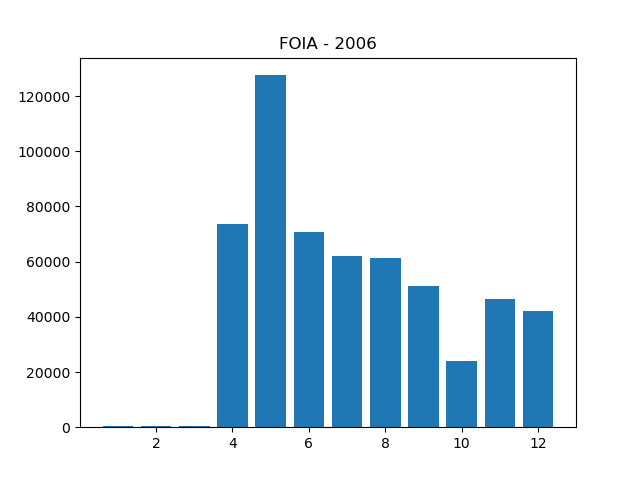
\includegraphics[width=\textwidth]{../../output/figures/annual_source_distribution/FOIA_data_dist_2006.png}
    \end{subfigure}
    \begin{subfigure}{.5\textwidth}
        \centering
        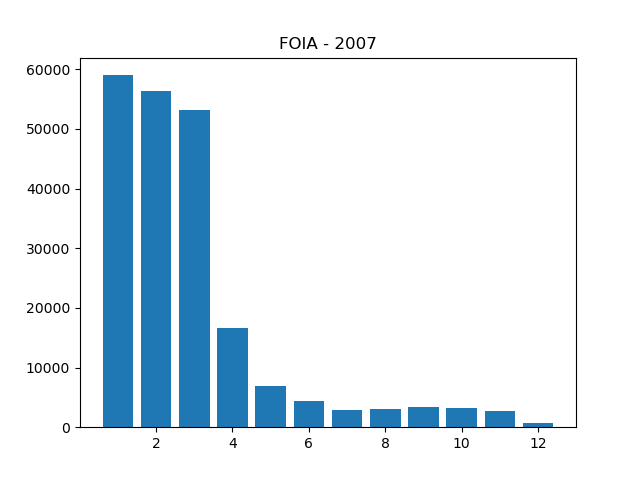
\includegraphics[width=\textwidth]{../../output/figures/annual_source_distribution/FOIA_data_dist_2007.png}
    \end{subfigure}
    \begin{subfigure}{.5\textwidth}
        \centering
        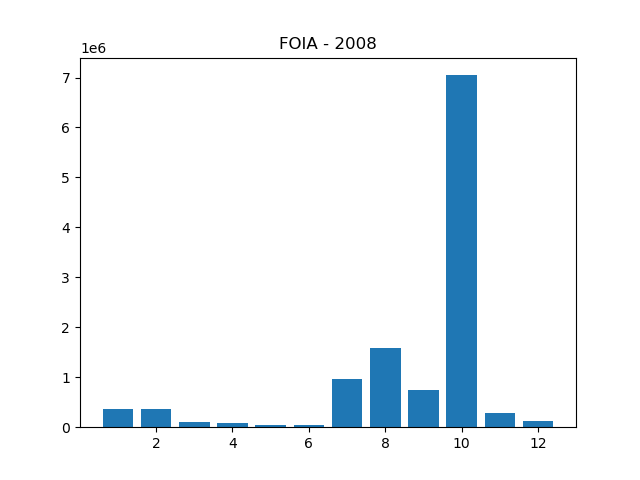
\includegraphics[width=\textwidth]{../../output/figures/annual_source_distribution/FOIA_data_dist_2008.png}
    \end{subfigure}
    \begin{subfigure}{.5\textwidth}
        \centering
        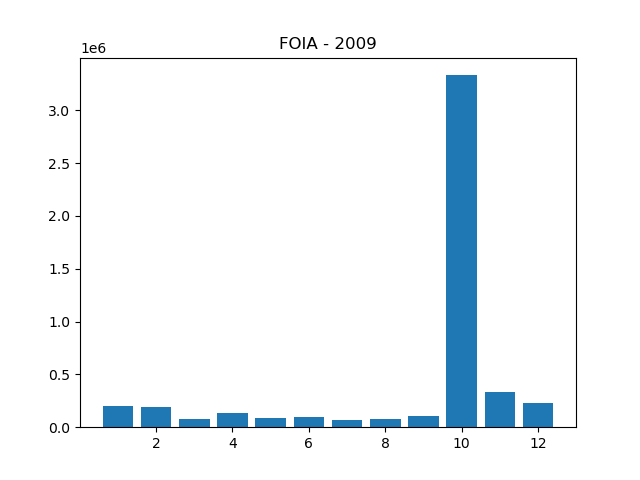
\includegraphics[width=\textwidth]{../../output/figures/annual_source_distribution/FOIA_data_dist_2009.png}
    \end{subfigure}
    \begin{subfigure}{.5\textwidth}
        \centering
        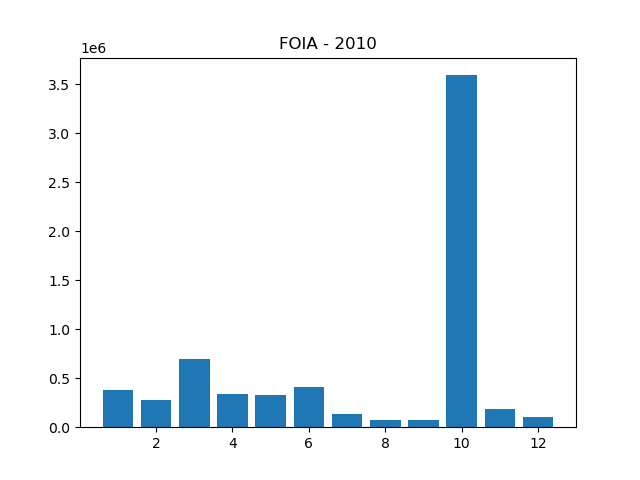
\includegraphics[width=\textwidth]{../../output/figures/annual_source_distribution/FOIA_data_dist_2010.png}
    \end{subfigure}
    \begin{subfigure}{.5\textwidth}
        \centering
        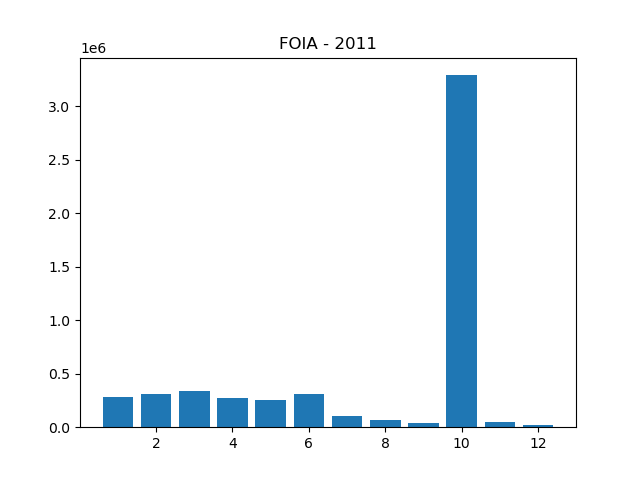
\includegraphics[width=\textwidth]{../../output/figures/annual_source_distribution/FOIA_data_dist_2011.png}
    \end{subfigure}
\end{figure}

\newpage 
\subsection*{FOIA 2012 through 2017}
\begin{figure}[H]
    \begin{subfigure}{.5\textwidth}
        \centering
        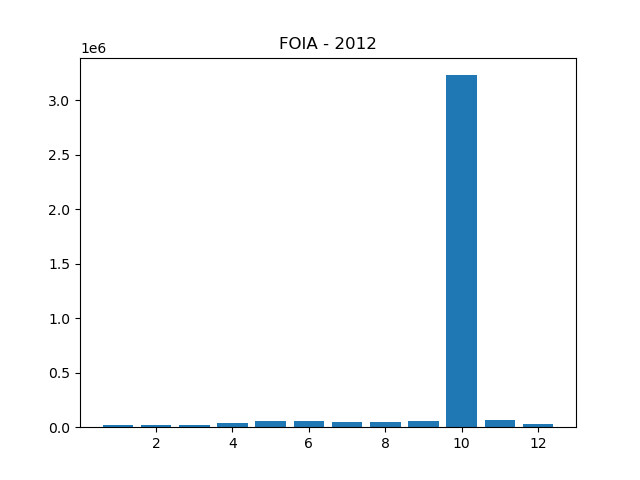
\includegraphics[width=\textwidth]{../../output/figures/annual_source_distribution/FOIA_data_dist_2012.png}
    \end{subfigure}
    \begin{subfigure}{.5\textwidth}
        \centering
        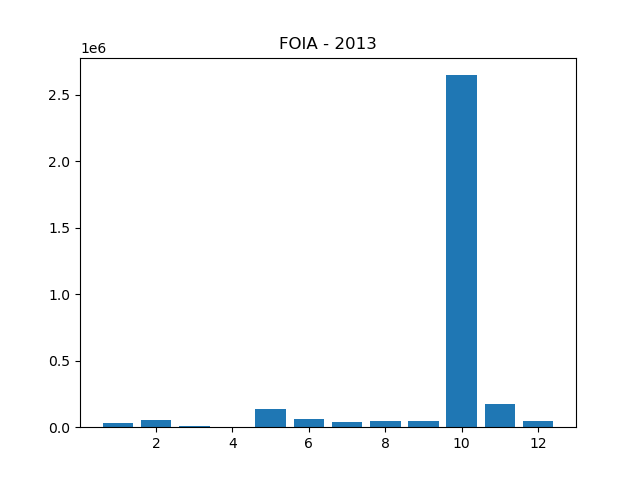
\includegraphics[width=\textwidth]{../../output/figures/annual_source_distribution/FOIA_data_dist_2013.png}
    \end{subfigure}
    \begin{subfigure}{.5\textwidth}
        \centering
        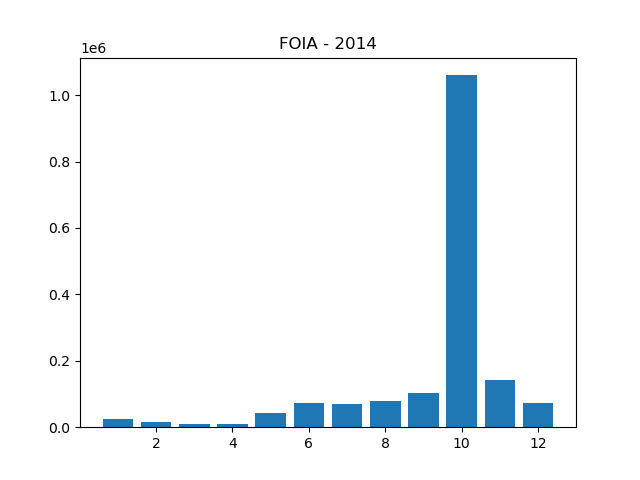
\includegraphics[width=\textwidth]{../../output/figures/annual_source_distribution/FOIA_data_dist_2014.png}
    \end{subfigure}
    \begin{subfigure}{.5\textwidth}
        \centering
        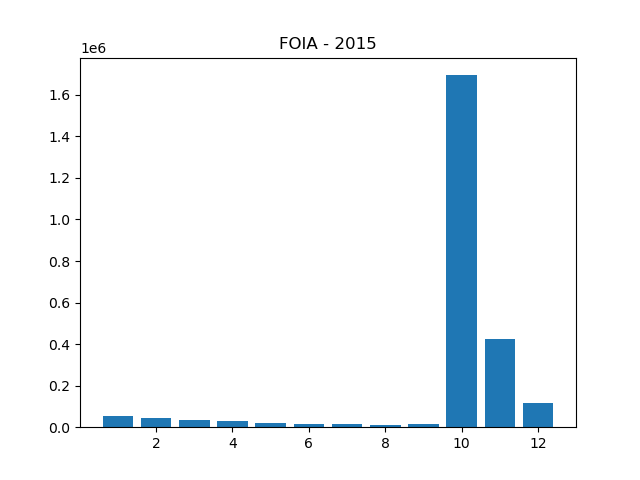
\includegraphics[width=\textwidth]{../../output/figures/annual_source_distribution/FOIA_data_dist_2015.png}
    \end{subfigure}
    \begin{subfigure}{.5\textwidth}
        \centering
        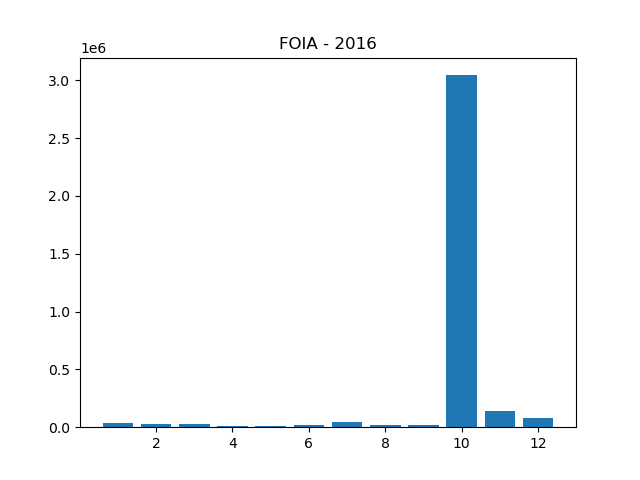
\includegraphics[width=\textwidth]{../../output/figures/annual_source_distribution/FOIA_data_dist_2016.png}
    \end{subfigure}
    \begin{subfigure}{.5\textwidth}
        \centering
        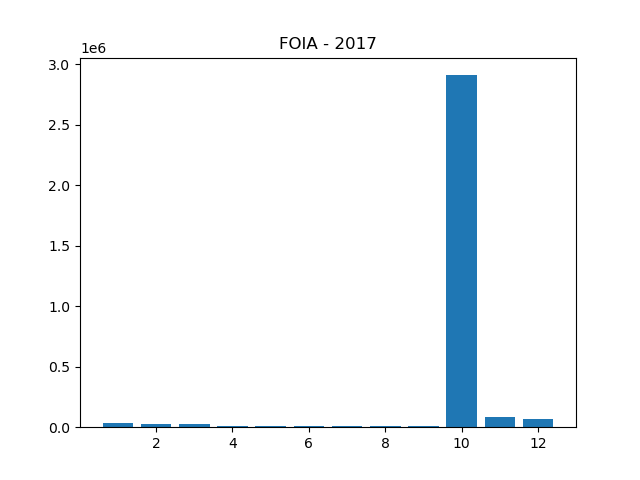
\includegraphics[width=\textwidth]{../../output/figures/annual_source_distribution/FOIA_data_dist_2017.png}
    \end{subfigure}
\end{figure}

\newpage 
\subsection*{FOIA 2018 through 2022}
\begin{figure}[H]
    \begin{subfigure}{.5\textwidth}
        \centering
        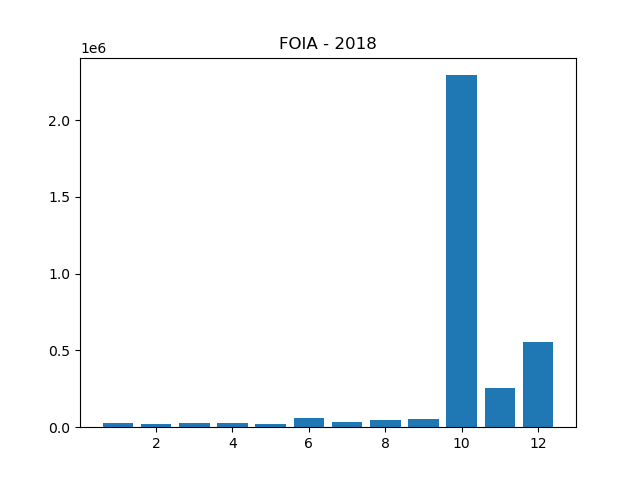
\includegraphics[width=\textwidth]{../../output/figures/annual_source_distribution/FOIA_data_dist_2018.png}
    \end{subfigure}
    \begin{subfigure}{.5\textwidth}
        \centering
        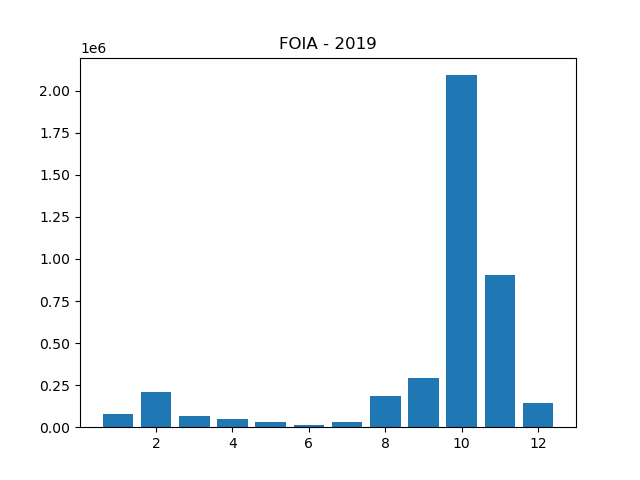
\includegraphics[width=\textwidth]{../../output/figures/annual_source_distribution/FOIA_data_dist_2019.png}
    \end{subfigure}
    \begin{subfigure}{.5\textwidth}
        \centering
        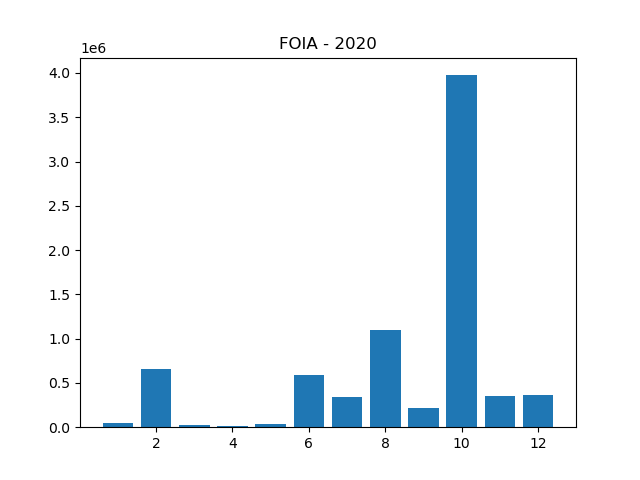
\includegraphics[width=\textwidth]{../../output/figures/annual_source_distribution/FOIA_data_dist_2020.png}
    \end{subfigure}
    \begin{subfigure}{.5\textwidth}
        \centering
        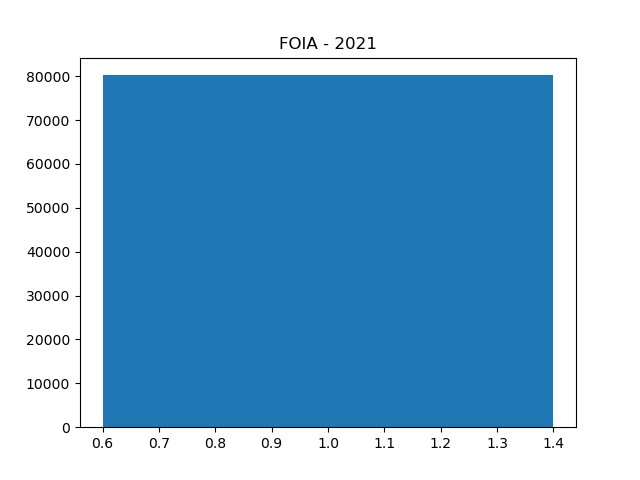
\includegraphics[width=\textwidth]{../../output/figures/annual_source_distribution/FOIA_data_dist_2021.png}
    \end{subfigure}
    \begin{subfigure}{.5\textwidth}
        \centering
        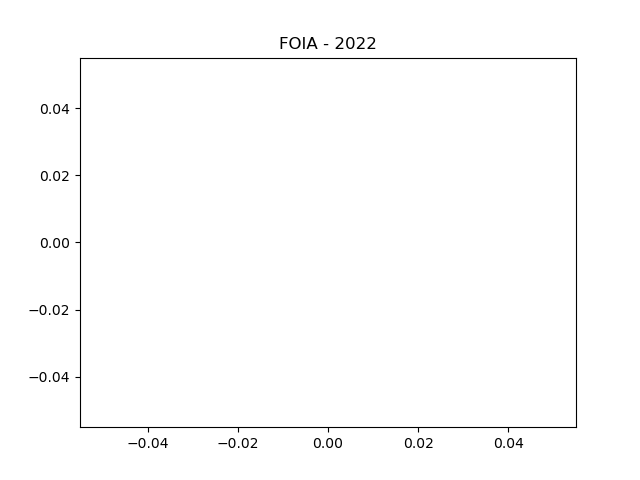
\includegraphics[width=\textwidth]{../../output/figures/annual_source_distribution/FOIA_data_dist_2022.png}
    \end{subfigure}
\end{figure}

\subsection*{Public 2006 through 2011}
\begin{figure}[H]
    \begin{subfigure}{.5\textwidth}
        \centering
        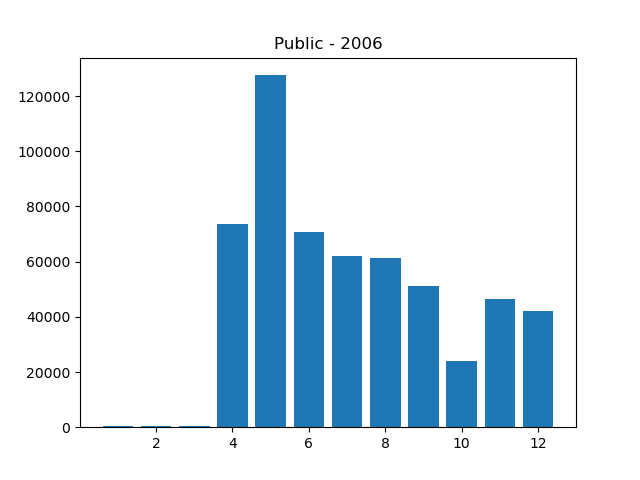
\includegraphics[width=\textwidth]{../../output/figures/annual_source_distribution/Public_data_dist_2006.png}
    \end{subfigure}
    \begin{subfigure}{.5\textwidth}
        \centering
        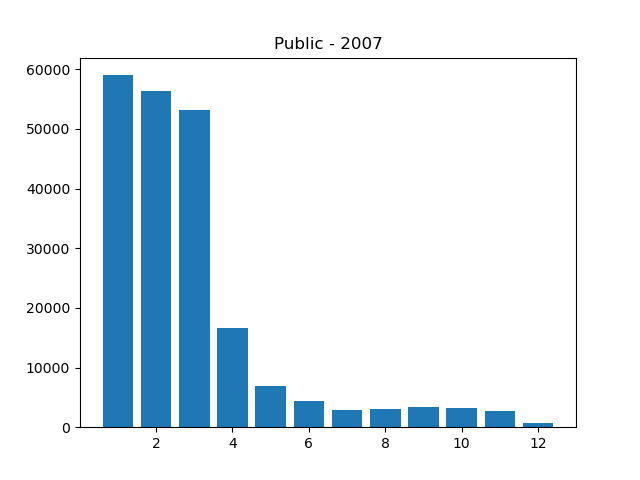
\includegraphics[width=\textwidth]{../../output/figures/annual_source_distribution/Public_data_dist_2007.png}
    \end{subfigure}
    \begin{subfigure}{.5\textwidth}
        \centering
        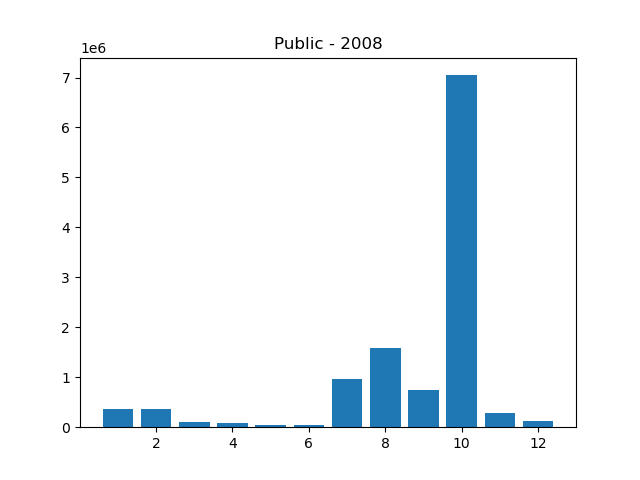
\includegraphics[width=\textwidth]{../../output/figures/annual_source_distribution/Public_data_dist_2008.png}
    \end{subfigure}
    \begin{subfigure}{.5\textwidth}
        \centering
        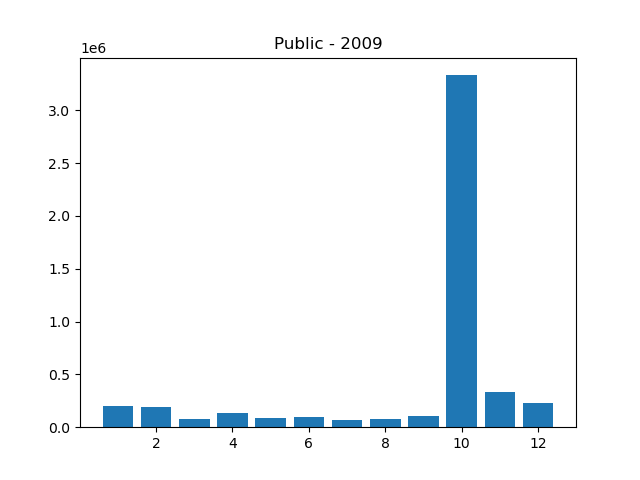
\includegraphics[width=\textwidth]{../../output/figures/annual_source_distribution/Public_data_dist_2009.png}
    \end{subfigure}
    \begin{subfigure}{.5\textwidth}
        \centering
        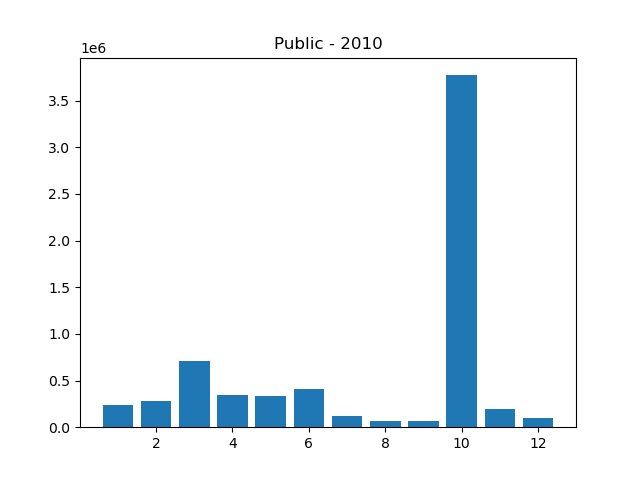
\includegraphics[width=\textwidth]{../../output/figures/annual_source_distribution/Public_data_dist_2010.png}
    \end{subfigure}
    \begin{subfigure}{.5\textwidth}
        \centering
        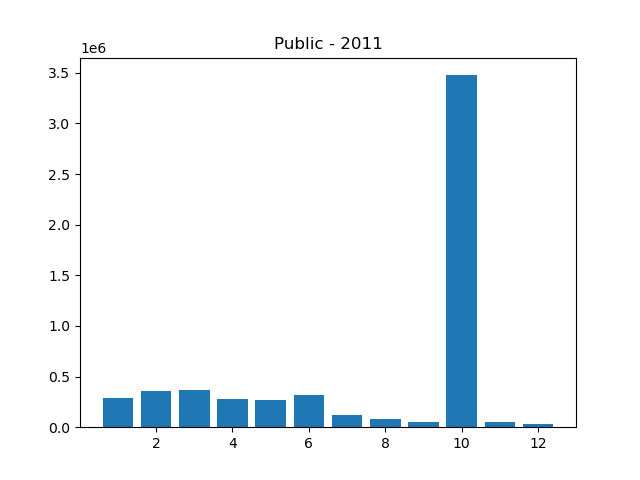
\includegraphics[width=\textwidth]{../../output/figures/annual_source_distribution/Public_data_dist_2011.png}
    \end{subfigure}
\end{figure}

\newpage 
\subsection*{Public 2012 through 2017}
\begin{figure}[H]
    \begin{subfigure}{.5\textwidth}
        \centering
        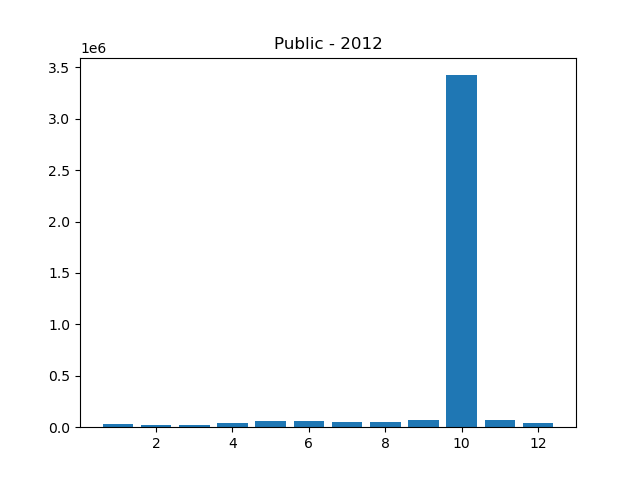
\includegraphics[width=\textwidth]{../../output/figures/annual_source_distribution/Public_data_dist_2012.png}
    \end{subfigure}
    \begin{subfigure}{.5\textwidth}
        \centering
        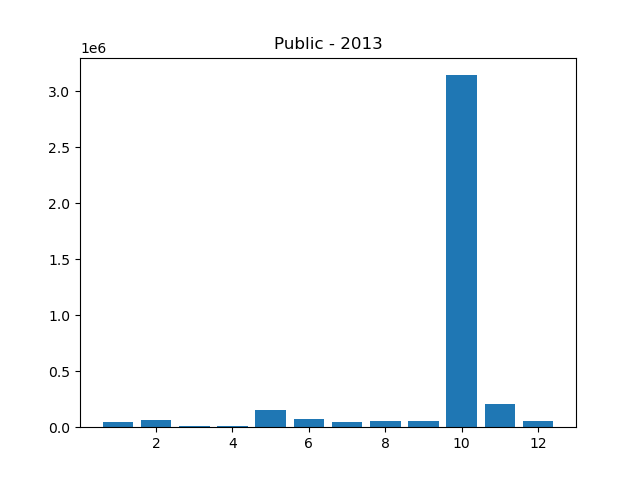
\includegraphics[width=\textwidth]{../../output/figures/annual_source_distribution/Public_data_dist_2013.png}
    \end{subfigure}
    \begin{subfigure}{.5\textwidth}
        \centering
        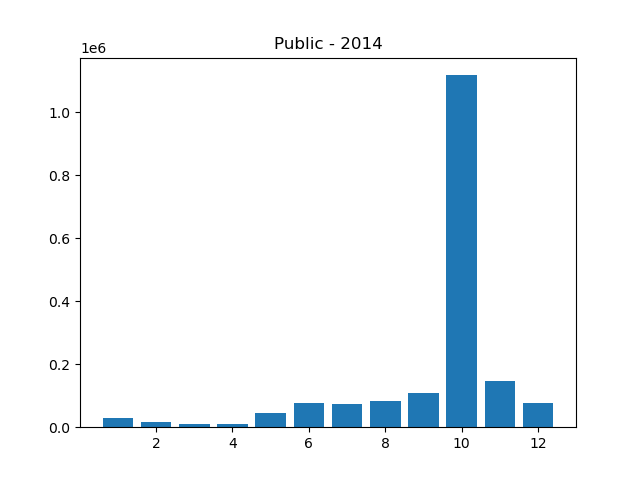
\includegraphics[width=\textwidth]{../../output/figures/annual_source_distribution/Public_data_dist_2014.png}
    \end{subfigure}
    \begin{subfigure}{.5\textwidth}
        \centering
        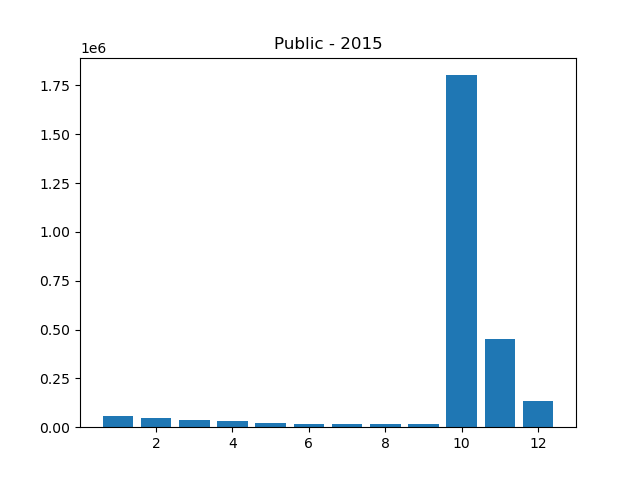
\includegraphics[width=\textwidth]{../../output/figures/annual_source_distribution/Public_data_dist_2015.png}
    \end{subfigure}
    \begin{subfigure}{.5\textwidth}
        \centering
        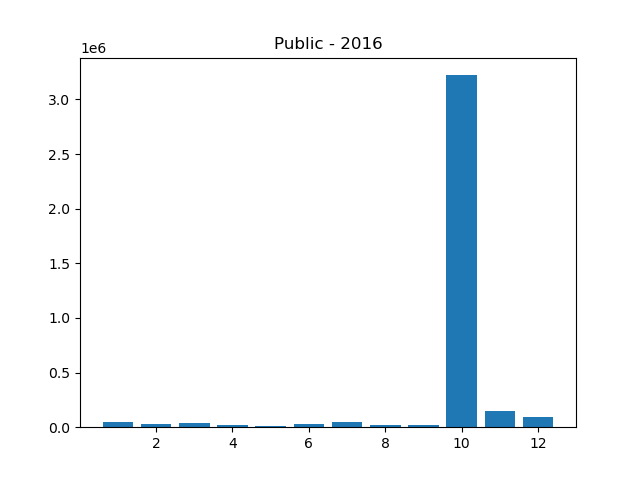
\includegraphics[width=\textwidth]{../../output/figures/annual_source_distribution/Public_data_dist_2016.png}
    \end{subfigure}
    \begin{subfigure}{.5\textwidth}
        \centering
        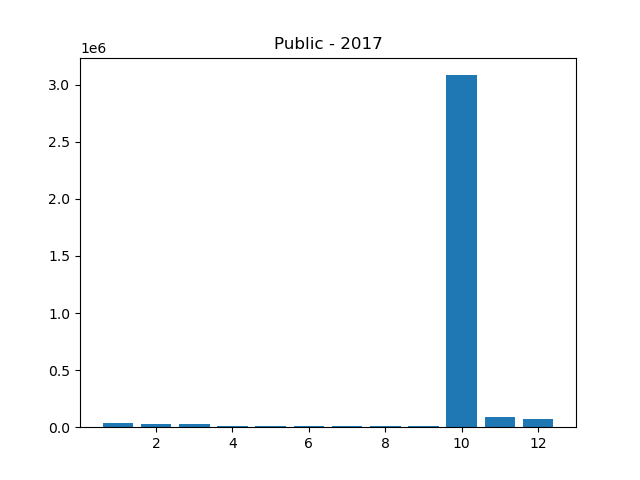
\includegraphics[width=\textwidth]{../../output/figures/annual_source_distribution/Public_data_dist_2017.png}
    \end{subfigure}
\end{figure}

\newpage 
\subsection*{Public 2018 through 2022}
\begin{figure}[H]
    \begin{subfigure}{.5\textwidth}
        \centering
        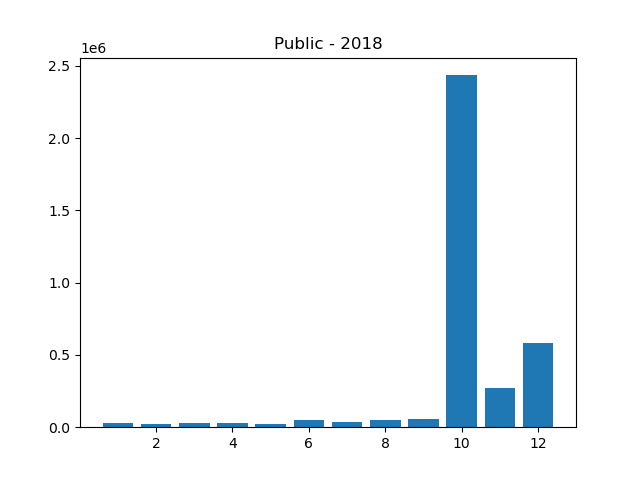
\includegraphics[width=\textwidth]{../../output/figures/annual_source_distribution/Public_data_dist_2018.png}
    \end{subfigure}
    \begin{subfigure}{.5\textwidth}
        \centering
        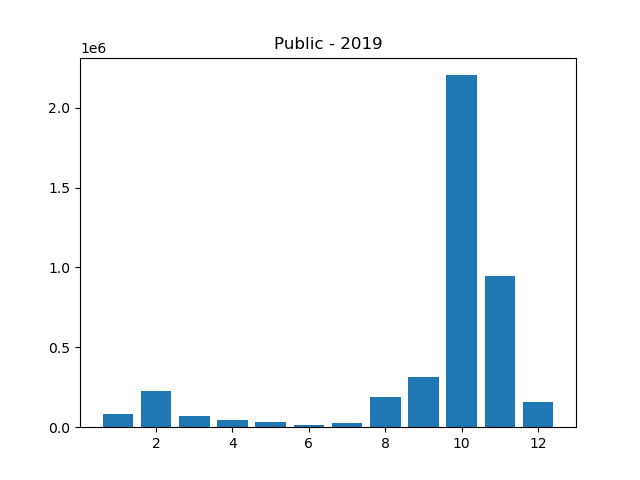
\includegraphics[width=\textwidth]{../../output/figures/annual_source_distribution/Public_data_dist_2019.png}
    \end{subfigure}
    \begin{subfigure}{.5\textwidth}
        \centering
        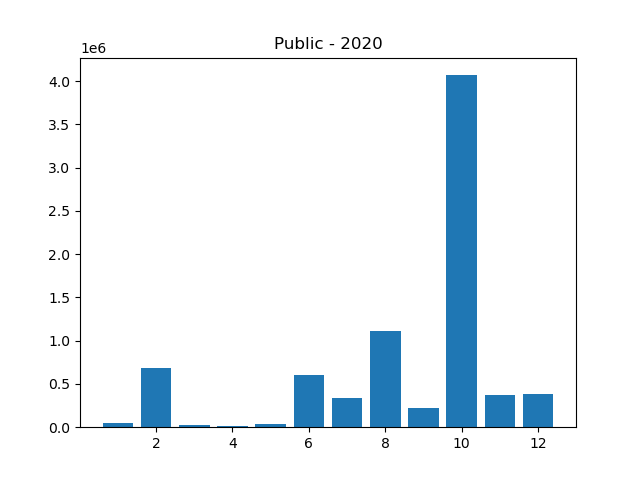
\includegraphics[width=\textwidth]{../../output/figures/annual_source_distribution/Public_data_dist_2020.png}
    \end{subfigure}
    \begin{subfigure}{.5\textwidth}
        \centering
        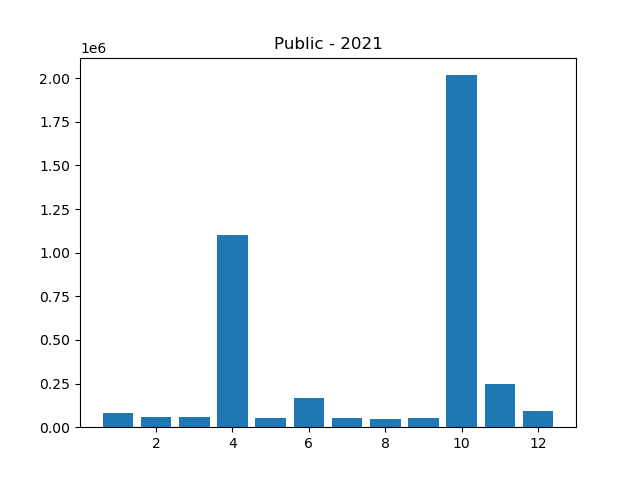
\includegraphics[width=\textwidth]{../../output/figures/annual_source_distribution/Public_data_dist_2021.png}
    \end{subfigure}
    \begin{subfigure}{.5\textwidth}
        \centering
        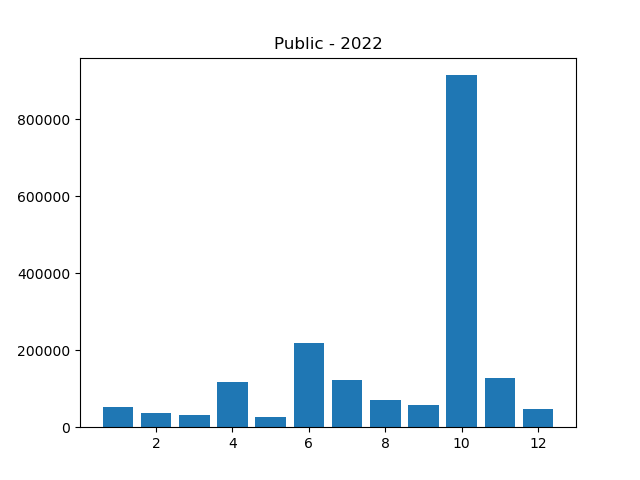
\includegraphics[width=\textwidth]{../../output/figures/annual_source_distribution/Public_data_dist_2022.png}
    \end{subfigure}
\end{figure}

\newpage 
\section*{Summary}
Beginning in 2010, the two different data sources diverge. The Public Data
has more records, a greater sum, larger mean payments, and often a higher maximum than does the 
FOIA'd data. 

\subsubsection*{Which states are most responsible for the difference?}
At first glance, it appears that there are many states that contribute significantly to the difference. However, upon close examination 
combined with the summary report (add ref), most of the states that show a subjectively large difference are the states that already receive the highest payout 
from these programs. States like Iowa, Indiana, Illinois, Indiana, Kansas, Nebraska, Ohio, and Texas are among the highest earning 
states from these programs, so seeing discrepancy of say, \$36 million in 2015 in Iowa is a small proportion of the over all earnings 
in the state that year. \\

While there are many small discrepancies that certainly add up, the most standout difference is D.C. 
In fact, D.C. is omitted entirely from the FOIA data, so that difference is simply the inclusion of that region.
For a complete look at the programs relevant to the D.C. region, see the county-level summary report (add ref).

\subsubsection*{Which porgrams are most responsible for the difference?}
There are 7 programs that are worth noting, listed \autoref{tab:topMovers}. Upon quick glance at the 
summary report, the first 6 are the largest programs year over year. The last program, the Market Access Program (MAP) 
is omitted from the FOIA data. In fact, the MAP coincides with only one jurisdiction - D.C. Therefore, it appears that 
the largest difference between the data sources is due to the omission of the Market Access Program in the FOIA data. 

\begin{table}[H]
    \caption{Programs with largest change}\label{tab:topMovers}
    \centering
    \begin{tabular}{|c|c|}
        \hline
        2746 & Supplemental Revenue Assistance Program \\ 
        2835 & Livestock Forage Program \\ 
        2837 & Price Loss Coverage Program \\ 
        2838 & Agricultural Risk Coverage \- County \\ 
        3132 & CRP \- ANNUAL RENTAL \\ 
        6742 & DCP \- Direct \\ 
        7610 & Market Access Program \\
        \hline
    \end{tabular}
\end{table}



\subsubsection*{Can we trust that Public 2021 and 2022 data is complete?}
Reviewing The summary statistics, 2021 appears to represent a fairly typical year, suggesting that it is complete in the Public Data. 2021 
is clearly incomplete in the FOIA data with only 80K records as opposed to the 4M records. \\ 
By the sum of payments, 2022 is on track as a middling year at \$13 billion. However, this occurs 
with only 1.8 million transactions, well below the 4 million that is typical of previous years. 
These two pieces of evidence appear to point in different directions. To resolve the issue, we turn to 
the distribution chart for Public 2022 data. In each year, October is the month with the highest total 
payouts, conicident with the beginning of the Federal Government fiscal year. While the total number of 
payments seems low, the distribution of such payments appears reasonable. We can compare this distribution 
to that of a known incomplete year. FOIA 2021 is known to be incomplete, and its distribution shows only January is 
included in the dataset. Seeing all months represented in the Public 2022 distribution is evidence in favor 
of the data being complete. While we cannot be sure, unless further information is uncovered, 
it seems a reasonable to proceed with 2022 data. 

\subsection*{Recommendations}
I recommend using the full set of Public data
\begin{itemize}
    \item Complete data in 2021, assumed complete in 2022
    \item Assuming the USDA will update the Public website, incorporating future years will be a straightforward process 
    \item Public Dataset appears to be more complete across the board, providing updated figures for each year and jurisdiction, while incorporating the Market Assistance Program in D.C. 
\end{itemize}

\newpage 
\section*{Appendix}
% add program code/name reference.
\begin{longtable}{ll}
\caption{Program Code / Name Lookup Table} \label{progCodeLookup} \\
\toprule
programCode & programName \\
\midrule
\endfirsthead
\caption[]{Program Code / Name Lookup Table} \\
\toprule
programCode & programName \\
\midrule
\endhead
\midrule
\multicolumn{2}{r}{Continued on next page} \\
\midrule
\endfoot
\bottomrule
\endlastfoot
2561 & LIVESTOCK COMPENSATION PROGRAM \\
\cline{1-2}
2564 & LIVESTOCK FORAGE DISASTER PROGRAM \\
\cline{1-2}
2567 & EMERG ASSIST LIVESTOCK BEES FISH (ELAP) \\
\cline{1-2}
2569 & LIVESTOCK INDEMNITY PROGRAM \\
\cline{1-2}
2571 & LIVESTOCK FORAGE DISASTER PROGRAM \\
\cline{1-2}
2572 & EMERG ASSIST LIVESTOCK BEES FISH (ELAP) \\
\cline{1-2}
2622 & NONINSURED ASSISTANCE PROGRAM \\
\cline{1-2}
2633 & LOSS ADJUSTER - NAP \\
\cline{1-2}
2677 & TASCP \\
\cline{1-2}
2687 & CROP DISASTER PROGRAM \\
\cline{1-2}
2695 & NON-INSURED ASSISTANCE PROG AUTHORIZED \\
\cline{1-2}
2746 & SUPPLEMENTAL REVENUE ASSISTANCE PROGRAM \\
\cline{1-2}
2747 & TREE ASSISTANCE PROGRAM \\
\cline{1-2}
2748 & TAAF FOR 2010 WEB BASED APPLICATION \\
\cline{1-2}
2749 & HURRICANE INDEMNITY PROGRAM, AUTHORIZED \\
\cline{1-2}
2750 & CRP BIOMASS CROP ASSISTANCE PROGRAM \\
\cline{1-2}
2752 & CROP DISASTER ASSISTANCE PROG AUTHORIZED \\
\cline{1-2}
2754 & SUPL REVENUE ASSISTANCE - RECOVERY ACT \\
\cline{1-2}
2765 & DAIRY ECONOMIC LOSS ASSISTANCE PROGRAM \\
\cline{1-2}
2767 & BCAP ANNUAL RENTAL WEB BASED \\
\cline{1-2}
2768 & BCAP COST SHARE WEB BASED \\
\cline{1-2}
2773 & GEOGRAPHIC DISADVANTAGED PROGRAM \\
\cline{1-2}
2775 & NON-INSURED ASSISTANCE PROGRAM \\
\cline{1-2}
2776 & CROP ASSISTANCE PROGRAM \\
\cline{1-2}
2782 & TAAF FOR 2011 WEB-BASED APPLICATION \\
\cline{1-2}
3050 & GRASSLANDS RESERVE PROGRAM \\
\cline{1-2}
3121 & CRP - EMERGENCY FORESTRY COST SHARE \\
\cline{1-2}
3125 & CRP - EMERGENCY FORESTRY ANNUAL RENTAL \\
\cline{1-2}
3130 & CRP PAYMENT - ANNUAL RENTAL \\
\cline{1-2}
3131 & CRP PAYMENT - ANNUAL RENTAL \\
\cline{1-2}
3340 & EMERGENCY FORESTRY RESTORATION PROGRAM \\
\cline{1-2}
4005 & CONSERVATION - EMERGENCY \\
\cline{1-2}
4020 & EMERGENCY CONSERV - SOUTHERN CALIFORNIA \\
\cline{1-2}
4040 & EMERGENCY CONSERVATION PROGRAM \\
\cline{1-2}
4205 & EMERGENCY CONSERVATION - FLOOD \\
\cline{1-2}
4305 & EMERGENCY CONSERVATION - TORNADO, AUTO \\
\cline{1-2}
4405 & EMERGENCY CONSERVATION - DROUGHT, AUTO \\
\cline{1-2}
4600 & EMERGENCY CONSERVATION - TECH SERVICES \\
\cline{1-2}
6390 & HAY GRAZING \\
\cline{1-2}
6395 & HAY GRAZING, MANAGED \\
\cline{1-2}
\multirow[t]{8}{*}{6740} & DIRECT PAYMENT - BARLEY \\
 & DIRECT PAYMENT - CORN \\
 & DIRECT PAYMENT - PEANUTS \\
 & DIRECT PAYMENT - RICE \\
 & DIRECT PAYMENT - SORGHUM \\
 & DIRECT PAYMENT - SOYBEANS \\
 & DIRECT PAYMENT - UPLAND COTTON \\
 & DIRECT PAYMENT - WHEAT \\
\cline{1-2}
6742 & DCP - DIRECT \\
\cline{1-2}
6744 & AVERAGE CROP REVENUE ELECTION-DIRECT \\
\cline{1-2}
6745 & COUNTER CYCLICAL PYMTS FROM SYS/36 \\
\cline{1-2}
6747 & DCP - COUNTER CYCLICAL \\
\cline{1-2}
6749 & AVERAGE CROP REVENUE ELECTION-ACRE \\
\cline{1-2}
7610 & MARKET ACCESS PROGRAM \\
\cline{1-2}
7900 & INDEMNITY PAYMENT - DAIRY \\
\cline{1-2}
8020 & INCOME LOSS - MILK, PART 2 \\
\cline{1-2}
2766 & BCAP MATCHING PYMNT WEB-BASE APPLICATION \\
\cline{1-2}
3101 & CRP PAYMENT - ANNUAL \\
\cline{1-2}
2736 & CROP DISASTER PROGRAM \\
\cline{1-2}
\multirow[t]{2}{*}{6740} & DIRECT PAYMENT - OATS \\
 & DIRECT PAYMENT - SUNFLOWER SEED \\
\cline{1-2}
3052 & GRASSLANDS RESERVE SPECIAL FUNDING \\
\cline{1-2}
4820 & EMERG CONSV - HURRICANE GULF OF MEXICO \\
\cline{1-2}
2715 & CROP DISASTER PROGRAM \\
\cline{1-2}
3128 & CRP - EMERGENCY FORESTRY ANNUAL RENTAL \\
\cline{1-2}
2755 & TREE ASSISTANCE PROGRAM - RECOVERY ACT \\
\cline{1-2}
2771 & DURUM WHEAT QUALITY PROGRAM \\
\cline{1-2}
\multirow[t]{2}{*}{6740} & DIRECT PAYMENT - FLAXSEED \\
 & DIRECT PAYMENT - SAFFLOWER SEED \\
\cline{1-2}
3110 & INCENTIVE PAYMENTS - RIPARIAN BUFFER \\
\cline{1-2}
4805 & EMERG CONSERVATION - HURRICANE, AUTO \\
\cline{1-2}
1001 & MARKET GAINS \\
\cline{1-2}
1005 & STORAGE FORGIVEN \\
\cline{1-2}
1030 & MARKET GAINS \\
\cline{1-2}
2300 & INTEREST PENALTY \\
\cline{1-2}
2380 & INTEREST PENALTY \\
\cline{1-2}
2521 & 05 - 07 LIVESTOCK INDEMNITY PROGRAM \\
\cline{1-2}
2525 & EMERGENCY LIVESTOCK FEED ASSISTANCE \\
\cline{1-2}
2556 & LIVESTOCK COMPENSATION PROGRAM - HURRICANE \\
\cline{1-2}
2561 & 05 - 07 LIVESTOCK COMPENSATION PROGRAM \\
\cline{1-2}
2687 & 01-02 CROP DISASTER ASSISTANCE PROGRAM \\
\cline{1-2}
2688 & TRADE ADJUSTMENT ASSISTANCE \\
\cline{1-2}
2695 & NONINSURED ASSISTANCE PROGRAM \\
\cline{1-2}
2697 & FLORIDA HURRICANE CHARLEY CITRUS DISASTER \\
\cline{1-2}
2714 & TREE ASSISTANCE PROGRAM - TIMBER \\
\cline{1-2}
2722 & TREE INDEMNITY PROGRAM \\
\cline{1-2}
2728 & SPECIALITY CROP HURRICANE DISASTER - CITRUS \\
\cline{1-2}
2730 & SPECIALITY CROP HURRICANE DISASTER - FRUIT/VEG \\
\cline{1-2}
2732 & SPECIALITY CROP HURRICANE DISASTER - NURSERY \\
\cline{1-2}
2733 & TREE ASSISTANCE PROGRAM - HURRICANE \\
\cline{1-2}
2736 & 05 - 07 CROP DISASTER ASSISTANCE \\
\cline{1-2}
2737 & 05 - 07 DAIRY DISASTER PROG \\
\cline{1-2}
3101 & CONSERVATION RESERVE PROGRAM - ANNUAL LAND RENTAL \\
\cline{1-2}
3105 & CONSERVATION RESERVE PROGRAM CANCELLATION, MISACTION \\
\cline{1-2}
3130 & CRP PAYMENT - ANNUAL PAYMENT \\
\cline{1-2}
3305 & AUTOMATED CONSERVATION RESERVE PROGRAM - COST SHARE \\
\cline{1-2}
3310 & CRP WETLAND RESTORATION PROGRAM \\
\cline{1-2}
3320 & CRP - PRACTICE INCENTIVE \\
\cline{1-2}
3325 & CRP - SIGNING INCENTIVE \\
\cline{1-2}
4005 & EMERGENCY CONSERVATION PROGRAM - OTHER \\
\cline{1-2}
4020 & EMERGENCY CONSERVATION - SOUTHERN CALIFORNIA \\
\cline{1-2}
4030 & EMERGENCY COMPENSATION PROGRAM - AGI \\
\cline{1-2}
4205 & EMERGENCY CONSERVATION PROGRAM - FLOOD \\
\cline{1-2}
4305 & EMERGENCY CONSERVATION PROGRAM - TORNADO \\
\cline{1-2}
4405 & EMERGENCY CONSERVATION PROGRAM - DROUGHT \\
\cline{1-2}
4805 & EMERGENCY CONSERVATION PROGRAM - HURRICANE \\
\cline{1-2}
4820 & EMERGENCY CONSERVATION - HURRICANE GULF MEXICO \\
\cline{1-2}
5201 & LOAN DEFICIENCY \\
\cline{1-2}
5207 & LOAN DEFICIENCY \\
\cline{1-2}
5280 & TTPP TOBACCO PRODUCER \\
\cline{1-2}
6395 & CRP ANNUAL RENTAL \\
\cline{1-2}
6740 & DIRECT AND COUNTER CYCLICAL PROG \\
\cline{1-2}
6745 & DIRECT AND COUNTER CYCLICAL PROG \\
\cline{1-2}
6801 & CRP ANNUAL RENTAL \\
\cline{1-2}
8020 & MILK INCOME LOSS CONTRACT II \\
\cline{1-2}
1000 & MARKET GAINS \\
\cline{1-2}
2310 & ADDITIONAL INTEREST PENALTY \\
\cline{1-2}
2564 & LIVESTOCK FORAGE DISASTER  PROGRAM \\
\cline{1-2}
2566 & LIVESTOCK INDEMNITY PROGRAM \\
\cline{1-2}
2721 & HURRICANE INDEMNITY PROGRAM \\
\cline{1-2}
2750 & BIOMASS CROP ASSISTANCE \\
\cline{1-2}
5281 & TOBACCO QUOTA HOLDER - INTEREST \\
\cline{1-2}
6390 & CRP ANNUAL RENTAL \\
\cline{1-2}
6742 & DCP PROGRAM - DIRECT PAYMENTS \\
\cline{1-2}
6744 & ACRE DIRECT PAYMENTS \\
\cline{1-2}
6747 & DCP PROGRAM - COUNTER CYCLICAL PAYMENTS \\
\cline{1-2}
7900 & DAIRY INDEMNITY PROGRAM \\
\cline{1-2}
5205 & LOAN DEFICIENCY \\
\cline{1-2}
2526 & LIVESTOCK ASSISTANCE PROGRAM \\
\cline{1-2}
2546 & FEED PROGRAM - AMERICAN INDIAN \\
\cline{1-2}
\multirow[t]{6}{*}{2688} & TRADE ADJUSTMENT - FISH, SALMON \\
 & TRADE ADJUSTMENT - FISH, SHRIMP \\
 & TRADE ADJUSTMENT - FRESH POTATOES \\
 & TRADE ADJUSTMENT - JUICE GRAPES \\
 & TRADE ADJUSTMENT - NUTS, LYCHEES \\
 & TRADE ADJUSTMENT - OLIVES \\
\cline{1-2}
5239 & EWE LAMB REPLACEMENT OR RETENTION \\
\cline{1-2}
\multirow[t]{7}{*}{5276} & TOBACCO TRANSITION PYMNT-AIR CURED, PROD \\
 & TOBACCO TRANSITION PYMNT-CIGAR, PROD \\
 & TOBACCO TRANSITION PYMNT-FLUE CURED,PROD \\
 & TOBACCO TRANSITION PYMNT-SUN CURED, PROD \\
 & TOBACCO TRANSITION PYMNT-VA FIRE CURED \\
 & TOBACCO TRANSITION PYMT-BURLEY, PROD \\
 & TOBACCO TRANSITION PYMT-FIRE CURED, PROD \\
\cline{1-2}
\multirow[t]{6}{*}{5277} & TOBACCO TRANSITION PYMNT-BURLEY, QUOTA \\
 & TOBACCO TRANSITION PYMNT-FLUECURED,QUOTA \\
 & TOBACCO TRANSITION PYMNT-SUN CURED,QUOTA \\
 & TOBACCO TRANSITION PYMT-AIR CURED, QUOTA \\
 & TOBACCO TRANSITION PYMT-CIGAR, QUOTA \\
 & TOBACCO TRANSITION PYMT-FIRE CURED,QUOTA \\
\cline{1-2}
8011 & INCOME LOSS - MILK \\
\cline{1-2}
8016 & INCOME LOSS TRANSITION - MILK \\
\cline{1-2}
2688 & TRADE ADJUSTMENT - AVOCADOS, FRESH \\
\cline{1-2}
4330 & EMERGENCY CONSERVATION PROGRAM - KANSAS TORNADOS \\
\cline{1-2}
2694 & TREE ASSISTANCE PROGRAM - MICHIGAN \\
\cline{1-2}
2712 & TREE ASSISTANCE PROGRAM - ORCHARDS \\
\cline{1-2}
3052 & GRASSLANDS RESERVE PROGRAM \\
\cline{1-2}
2753 & BIOMASS CROP ASSISTANCE TITLE 1 CROP RESIDUE \\
\cline{1-2}
3120 & CRP - EMERGENCY FORESTRY ANNUAL RENTAL \\
\cline{1-2}
2832 & LIVESTOCK INDEMNITY PROGRAM \\
\cline{1-2}
2833 & EMERG ASSIST LIVESTOCK BEES FISH (ELAP) \\
\cline{1-2}
2834 & TREE ASSISTANCE PROGRAM \\
\cline{1-2}
2835 & LIVESTOCK FORAGE PROGRAM \\
\cline{1-2}
2837 & PRICE LOSS COVERAGE PROGRAM \\
\cline{1-2}
2838 & AGRICULTURAL RISK COVERAGE PROG - COUNTY \\
\cline{1-2}
2840 & AGRICULTURAL RISK COVERAGE - INDIVIDUAL \\
\cline{1-2}
2862 & AGRICULTURAL RISK COVERAGE -COUNTY PILOT \\
\cline{1-2}
2867 & MARKET FACILITATION PROGRAM - CROPS \\
\cline{1-2}
2868 & MARKET FACILITATION PROGRAM - DAHG \\
\cline{1-2}
2870 & MARKET FACILITATION PROG-SPECIALTY CROPS \\
\cline{1-2}
2872 & TREE ASSISTANCE PROGRAM \\
\cline{1-2}
2875 & DIS/WH2 2019 WFHURRINDEMP \\
\cline{1-2}
2877 & TMP/MFP 2019 NON SPECIALTY CROPS \\
\cline{1-2}
2878 & TMP/MFP 2019 SPECIALITY CROPS \\
\cline{1-2}
2879 & TMP/MFP 2019 LIVESTOCK \\
\cline{1-2}
2880 & TMP/MFP 2019 NON-SPECIALITY CROPS-A \\
\cline{1-2}
2881 & WML/WML 19 WHIP MILK LOSS \\
\cline{1-2}
2888 & WHIP PLUS 3 ASSISTANCE \\
\cline{1-2}
2907 & SEAFOOD TRADE RELIEF PROGRAM \\
\cline{1-2}
2920 & NAP REGULAR WEB-BASED \\
\cline{1-2}
3070 & GRASSLANDS RESERVE PROGRAM \\
\cline{1-2}
3132 & CRP PAYMENT - ANNUAL RENTAL \\
\cline{1-2}
3338 & CRP TRANSITION INCENTIVES PRGM \\
\cline{1-2}
3353 & CRP - CHESAPEAKE BAY INCENTIVE \\
\cline{1-2}
3359 & CRP PRACTICE INCENTIVES PAYMENT \\
\cline{1-2}
4042 & EMERGENCY CONSERVATION PROGRAM FY17 \\
\cline{1-2}
4050 & EMERGENCY CONSERVATION PROGRAM STAFFORD \\
\cline{1-2}
4056 & ECP COST SHARE FY 2018 \\
\cline{1-2}
4058 & ECP/HMC COST SHARE FY19 \\
\cline{1-2}
4064 & WECPCSCOF \\
\cline{1-2}
4920 & CFAPCARES \\
\cline{1-2}
4925 & CFAPCCCCA \\
\cline{1-2}
4926 & CFAPCCA2 \\
\cline{1-2}
\multirow[t]{3}{*}{6150} & CCC ORGANIC COST SHARE - CROPS \\
 & CCC ORGANIC COST SHARE - LIVESTOCK \\
 & CCC ORGANIC COST SHARE - WILD CROPS \\
\cline{1-2}
6152 & CCC ORGANIC COST SHARE FEES - HANDLING \\
\cline{1-2}
8025 & MARGIN PROTECTION PROGRAM - DAIRY \\
\cline{1-2}
\multirow[t]{2}{*}{8053} & DAIRY MARGIN COVERAGE \\
 & DAIRY MARGIN COVERAGE PROGRAM \\
\cline{1-2}
2767 & BIOMASS CROP ASSISTANCE - ANNUAL RENTAL \\
\cline{1-2}
2864 & WILDFIRES AND HURRICANES INDEMNITY PROG \\
\cline{1-2}
2886 & WHIP 791 \\
\cline{1-2}
3344 & EMERGENCY FOREST RESTORATION STAFFORD \\
\cline{1-2}
3352 & CRP - TREE THINNING INCENTIVE PROGRAM \\
\cline{1-2}
4060 & ECPCOF \\
\cline{1-2}
4921 & CFAPCARES2 \\
\cline{1-2}
6152 & ORGANIC COST SHARE FEES- ST ORG PGM FEES \\
\cline{1-2}
6752 & DCP - DIRECT \\
\cline{1-2}
2757 & TREE ASSISTANCE REGULAR \\
\cline{1-2}
3110 & CRP - RIPARIAN BUFFER INCENTIVE \\
\cline{1-2}
6730 & MARKET LOSS ASSISTANCE \\
\cline{1-2}
7510 & 90 DAY RULE PAYMENTS \\
\cline{1-2}
3307 & CRP COST-SHARE WEB-BASED - COF \\
\cline{1-2}
3361 & CRP - CONTINUOUS PIP \\
\cline{1-2}
4041 & ECP PRIVATE SECTOR TECHNICAL ASSISTANCE \\
\cline{1-2}
2852 & GEOGRAPHIC DISADVANTAGED PROGRAM \\
\cline{1-2}
2858 & GEOGRAPHIC DISADVANTAGED PROGRAM \\
\cline{1-2}
2860 & GEOGRAPHIC DISADVANTAGED PROGRAM \\
\cline{1-2}
2865 & GEOGRAPHIC DISADVANTAGED PROGRAM \\
\cline{1-2}
2874 & GEOGRAPHIC DISADVANTAGED PROGRAM \\
\cline{1-2}
3357 & ERP/HMC COST SHARE FY19 \\
\cline{1-2}
7902 & DIPP WEB-BASED \\
\cline{1-2}
2570 & LIVESTOCK INDEMNITY PROGRAM \\
\cline{1-2}
8030 & MARGIN PROTECTION  - DAIRY \\
\cline{1-2}
2440 & COTTON TRANSITION ASSISTANCE PROGRAM \\
\cline{1-2}
2751 & BCAP PRIVATE SECTOR TECHNICAL ASSISTANCE \\
\cline{1-2}
2761 & TREE ASSISTANCE PROGRAM - RECOVERY ACT \\
\cline{1-2}
2762 & SUPPLEMENTAL REVENUE ASSISTANCE PROGRAM \\
\cline{1-2}
2763 & SUPL REVENUE ASSISTANCE - RECOVERY ACT \\
\cline{1-2}
2823 & GEOGRAPHIC DISADVANTAGED PROGRAM \\
\cline{1-2}
2832 & LIVESTOCK INDEMINITY PAYMENTS PROGRAM \\
\cline{1-2}
2836 & GEOGRAPHIC DISADVANTAGED PROGRAM \\
\cline{1-2}
2837 & PRICE LOSS COVERAGE \\
\cline{1-2}
2843 & NON-INSURED ASSISTANCE FROST FREE \\
\cline{1-2}
3129 & CRP - EMERGENCY FORESTRY ANNUAL RENTAL \\
\cline{1-2}
3133 & CRP - EMERGENCY FORESTRY COST SHARE \\
\cline{1-2}
3347 & EFRP SANDY STAFFORD COST SHARE \\
\cline{1-2}
3351 & CRP CHESAPEAKE BAY INCENTIVE \\
\cline{1-2}
2566 & LIVESTOCK INDEMNITY - TRUST FUND \\
\cline{1-2}
2779 & HAWAII SUGAR DISASTER PROGRAM \\
\cline{1-2}
2775 & WEB-BASED NAP \\
\cline{1-2}
2838 & ARC PROGRAM-COUNTY COVERAGE \\
\cline{1-2}
2840 & ARC PROGRAM INDIVIDUAL COVERAGE \\
\cline{1-2}
2862 & ARC PROGRAM-COUNTY PILOT COVERAGE \\
\cline{1-2}
2863 & TREE ASSISTANCE PROGRAM - PECAN \\
\cline{1-2}
2869 & WILDFIRES AND HURRICANES INDEMNITY PROG \\
\cline{1-2}
2876 & TREE ASSISTANCE PROGRAM \\
\cline{1-2}
2881 & WHIP MILK LOSS \\
\cline{1-2}
2889 & WHIP - SUGAR BEET COOPERATIVES \\
\cline{1-2}
3352 & TREE THINNING INCENTIVE \\
\cline{1-2}
4056 & ECP HURICNS HARVEY/IRMA/MARIA-CSTSHRFY18 \\
\cline{1-2}
4063 & ECPSFCOF \\
\cline{1-2}
2441 & COTTON GINNING COST SHARE PROGRAM \\
\cline{1-2}
2854 & BIOFUEL INFRASTRUCTURE PROGRAM \\
\cline{1-2}
3053 & GRASSLAND RESERVE PROGRAM-ANNUAL RENTAL \\
\cline{1-2}
3353 & CHESAPEAKE BAY INCENTIVE \\
\cline{1-2}
2442 & COTTON TRANSITION ASSISTANCE PROGRAM \\
\cline{1-2}
\multirow[t]{2}{*}{6140} & AMA ORGANIC COST SHARE - CROPS \\
 & AMA ORGANIC COST SHARE - LIVESTOCK \\
\cline{1-2}
6754 & AVERAGE CROP REVENUE ELECTION - DIRECT \\
\cline{1-2}
2580 & LIVESTOCK FORAGE DISASTER PROGRAM \\
\cline{1-2}
2785 & GEOGRAPHIC DISADVANTAGED PROGRAM \\
\cline{1-2}
2789 & GEOGRAPHIC DISADVANTAGED PROGRAM \\
\cline{1-2}
2441 & COTTON GINNING COST SHARE \\
\cline{1-2}
2861 & SUPPLEMENTAL REVENUE ASSISTANCE PROGRAM \\
\cline{1-2}
2866 & WILDFIRES AND HURRICANES INDEMNITY PROG \\
\cline{1-2}
1225 & ECONOMIC ADJUSTMENT ASSIST-UPLAND COTTON \\
\cline{1-2}
3356 & CRP FOREST INVENTORY PILOT PROGRAM \\
\cline{1-2}
2887 & FARM RANCHERS PROGRAM \\
\cline{1-2}
2908 & QUALITY LOSS ADJUSTMENT PROGRAM \\
\cline{1-2}
3358 & CRP FOREST MANAGEMENT INCENTIVE \\
\cline{1-2}
3364 & EFPSTACSOF \\
\cline{1-2}
3365 & ERFMCFSOF \\
\cline{1-2}
4061 & WECPCOF \\
\cline{1-2}
4062 & WECP17OF \\
\cline{1-2}
4922 & CFAPCARES2.1 \\
\cline{1-2}
4923 & CFAP3 - LTU \\
\cline{1-2}
4924 & CFAP3 - TUP \\
\cline{1-2}
8055 & DMC PRGM-SUPPLEMENTAL \\
\cline{1-2}
8286 & PANDEMIC ASST-TIMBER HARVESTERS/HAULERS \\
\cline{1-2}
8287 & PANDEMIC LIVESTOCK INDEMNITY PROGRAM \\
\cline{1-2}
3360 & CRP CLEAR30 MAINT PRGM \\
\cline{1-2}
8292 & SPOT MARKET HOG PANDEMIC PROGRAM \\
\cline{1-2}
2436 & EMGNCY RELIEF PROGRAM-SPECIALITY CROPS \\
\cline{1-2}
2437 & EMGNCY RELIEF PRGM-NONSPECIALITY CROPS \\
\cline{1-2}
2882 & ORIENTAL FRUIT FLY \\
\cline{1-2}
2885 & PECAN TREES - ADDTNL SUPLMNTL APPROP \\
\cline{1-2}
2911 & EMERGENCY LIVESTOCK RELIEF PROGRAM \\
\cline{1-2}
2921 & FARM RANCHERS PROGRAM \\
\cline{1-2}
4929 & CORONAVIRUS AID, CCC CHARTER ACT (OLP) \\
\cline{1-2}
8291 & ORGANIC and TRANSITIONAL EDU and CERT PRGM \\
\cline{1-2}
8293 & FOOD SAFETY CERTFCTN-SPECIALITY CROPS \\
\cline{1-2}
4053 & ECP SANDY STAFFORD COST SHARE \\
\cline{1-2}
2760 & TREE ASSISTANCE PROGRAM \\
\cline{1-2}
3126 & CRP - EMERGENCY FORESTRY COST SHARE \\
\cline{1-2}
5260 & GRAZE-OUT - BARLEY \\
\cline{1-2}
3349 & CRP HONEY BEE INCENTIVE PAYMNTS \\
\cline{1-2}
4927 & CARES ACT (OLP) \\
\cline{1-2}
4928 & CORONAVIRUS AID, CCC CHARTER ACT (OLP) \\
\cline{1-2}
\multirow[t]{2}{*}{5261} & ACREAGE GRAZING PAYMENTS - TRITICALE \\
 & ACREAGE GRAZING PAYMENTS - WHEAT \\
\cline{1-2}
5288 & TTPP - TOBACCO BURLEY \\
\cline{1-2}
2853 & BIOMASS CROP ASSIST COLLECTION MATCH PAY \\
\cline{1-2}
2759 & TREE ASSISTANCE MICHIGAN \\
\cline{1-2}
6753 & DCP - COUNTER CYCLICAL \\
\cline{1-2}
2581 & LIVESTOCK INDEMNITY - TRUST FUND \\
\cline{1-2}
4030 & ECP - ADJUSTED GROSS INCOME \\
\cline{1-2}
6740 & DIRECT PAYMENT - CANOLA SEED \\
\cline{1-2}
5260 & GRAZE-OUT - WHEAT \\
\cline{1-2}
3362 & EFRPCSOF \\
\cline{1-2}
3056 & GRASSLAND RESERVE PROGRAM - EASEMENT \\
\cline{1-2}
5288 & TTPP - TOBACCO FLUE CURED \\
\cline{1-2}
6140 & AMA ORGANIC COST SHARE - WILD CROPS \\
\cline{1-2}
6740 & DIRECT PAYMENT - SESAME \\
\cline{1-2}
\end{longtable}


\end{document}